\lhead{\begin{tikzpicture}[remember picture, overlay]
    \node [anchor=100,inner sep=0] (imagenIZQUIERDA) at (current page header area.north){
\includegraphics[width=18cm]{img/Encabezado.PNG}};
    \end{tikzpicture}}
    \rhead{Pilar-Martinez}
    \rfoot{\begin{tikzpicture}[remember picture, overlay]
    \node [anchor=140,inner sep=0] (imagenDERECHA) at (current page footer area.south){
\includegraphics[width=18cm]{img/Foot.PNG}};
    \end{tikzpicture}}
    %----------------------------------------------------------------------------------------
    \lfoot{ \thepage}
    % \renewcommand{\labelenumi}{\alph{enumi}.)} 
    %----------------------------------------------------------------------------------------
    %----------------------------------------------------------------------------------------
    %	TITLE SECTION
    %----------------------------------------------------------------------------------------
    
    \setlength{\droptitle}{-5\baselineskip} % Move the title up
    \title{\textbf{Estudio de tiempos y movimientos en el ensamble de un circuito electrónico utilizando diferentes métodos para su optimización }} % Article title
    
     \author{ 
     \textsc{Pilar Martinez, Oscar Jesús}\\ 
    %  Afiliación:
     \texttt{ Instituto Tecnológico de Querétaro } \\ 
     \texttt{Tecnológico Nacional de México} \\ 
     \texttt{ Querétaro, México}\\ 
     \texttt{pilaroscar2@gmail.com} 
     \and 
     \textsc{Ángeles-Hurtado, Luis Alberto}\\ 
    %  Afiliación:
     \texttt{ Instituto Tecnológico de Querétaro } \\ 
     \texttt{ Tecnológico Nacional de México } \\ 
     \texttt{Querétaro, México}\\ 
     \texttt{alb3rt0.ah@gmail.com} 
    }
    
    
    %----------------------------------------------------------------------------------------
    
    % \begin{document}
    
    % Print the title
    \maketitle
    \thispagestyle{fancy}
    
    %----------------------------------------------------------------------------------------
    %	ARTICLE CONTENTS
    %----------------------------------------------------------------------------------------
    
    % \section*{Resumen}
    % \textit{Palabras clave:}
    % El resumen (ancho de página) deberá contener entre 100 y 200 palabras tipo Adobe Devangari 11 puntos.
    
    \begin{abstract}
    \noindent 
    El resumen (ancho de página) deberá contener entre 100 y 200 palabras tipo Adobe Devangari 11 puntos.
    
    \end{abstract}
    % 
    % 
    \textbf{\textit{Palabras clave}}: {First keyword should be the corresponding to the research area according with the authors guide. Maximum of 6 keywords.}
    % \keywords{First keyword should be the corresponding to the research area according with the authors guide. Maximum of 6 keywords.}
    
    \section{Introducción}
    
    % Define estudio de tiempos y movimientos
    % define que es ensamble
    % define que es circuito electronico
    % define el metodo de tiempos predeterminados
    \begin{itemize}
        \item El estudio de tiempos y movimientos, se trata del análisis de todos los métodos, materiales, herramientas e instalaciones utilizadas o que se han de utilizar en la ejecución de un trabajo, el cual consta de cuatro etapas, la primera ayuda a encontrar la forma mas económica de realizar el trabajo, la segunda consta de la normalización tanto de métodos, materiales, así como las herramientas e instalaciones, el tercero tiene como objetivo determinar de manera exacta el tiempo que le lleva a una persona a realizar un trabajo de manera competente y a una marcha normal, como cuarto y ultima etapa debe de existir una ayuda al aprendizaje del operario en cuestión a nuevos métodos implementados o que serán implementados, para poder mejorar en todos y cada uno de los casos debemos de tener en consideración todos los factores posibles que influyan en el proceso. estos análisis se pueden ver utilizados en la ejecución de un ensamble ya que consisten en diversos componentes específicos para lograr una función adecuada, esta pieza requiere de un diseño detallado y de una correcta planificación, además su eficiencia puede verse modificada mediante ajustes del diseño y la selección adecuada de sus componentes, como lo es el caso de un circuito eléctrico, pues este esta basado en la planificación de un diseño, consta de diversos componentes como lo son las resistencias, capacitores, inductores, transitores, este debe estar ensamblado con ayuda de herramientas, pinzas, multimetros, soldadores, lo que mas importa es la intervención de la mano de obra, se debe de contar con un personal capacitado y adecuado a los factores a considerar. Para lograr lo antes mencionado debemos basarnos en un conjunto de reglas o métodos para determinar con anticipación la secuencia de los sucesos, el cual es llamado Sistema de Tiempos Predeterminados (STP), los cuales a su vez se basan en therblings, los therblings son movimientos básicos de las manos y el cuerpo identificados por Frank y Lillian Gilbreth para analizar y optimizar tareas manuales en ingeniería industrial. Incluyen acciones como buscar, seleccionar, agarrar, mover, sostener, y ensamblar. Utilizados en el ensamble, los therbligs permiten descomponer tareas, eliminar movimientos innecesarios, estandarizar procedimientos y mejorar la eficiencia y productividad en los procesos de producción.
    \end{itemize}
    % 
    % 
    \section{Justificación}
    
    \begin{itemize}
        \item A lo largo de la historia de la industria, se ha trabajado con el estudio de tiempos y movimientos.
        En la Primera revolución industrial (1760-1840) que fue cuando se introdujo la máquina de vapor y la creación de fabricas y sistemas de producción masiva, en esta etapa no estaba desarrollado formalmente el estudio de tiempos y movimientos, sin embargo a medida que las fabricas producían los dueños buscaban la eficiencia y maximizar la producción, conforme la industria crecía el desarrollar el estudio de tiempos y movimientos se hacía más relevante.
        Posteriormente en la Segunda Revolución Industrial (1870-1914) \cite{RevoluciónIndustrial} la cual se caracterizo por el uso del acero, electricidad y producción en masa así como el, desarrollo del motor de combustión interna y la aparición de la cadena de montaje. Dentro de esta etapa tenemos la importante participación de Frederick Winslow Taylor quien es nombrado el "Padre" del estudio de tiempos y movimientos, es conocido así por su Obra "Principios de la administración científica" (1911) sentó las bases de la gestión científica. Taylor llevó a cabo estudios detallados para determinar más eficiente de realizar una tarea, eliminando movimientos innecesarios\cite{Taylor}. Frank y Lillian Gilbreth también aportaron destacadamente, desarrollando el estudio de movimientos y la técnica del micro-movimiento, que fragmentar los movimientos en tareas más pequeñas para optimizar cada paso.\cite{Gilberth}
       La revoluciones industriales nos han dado pie a procesos de manufactura los cuales ocupamos hoy en día, sin los procesos de manufactura nos sería difícil mantener una empresa funcionando.
       Para determinar la cantidad de empresas de manufactura hay en el mundo es un tanto complejo debido a la diversidad de esta industria Sin embargo, informes de entidades como el Banco Mundial ofrecen una visión general. "En 2019, el valor total de la producción manufacturera a nivel mundial alcanzó los 13,739,251 millones de dólares". Este sorprendente valor refleja la dimensión del sector manufacturero y su importante papel en la economía global, aunque no proporciona un número específico de empresas. Según McKinsey, "la manufactura constituye aproximadamente el 16 por ciento del PIB global y emplea al 14 por ciento de la fuerza laboral mundial". 
       En México ocupamos el séptimo lugar en  producción manufacturera mundial, con un valor de 314,701 millones de dólares en 2020. Este crecimiento indica una expansión y desarrollo constante en el sector manufacturero del país, que incluye diversas industrias como la automotriz, aeroespacial, y de dispositivos médicos. \cite{McKinsey}.
       Con ayuda del estudio de tiempos y movimientos, buscamos realizar una mejora continua utilizando un análisis detallado de cada uno de los componentes que conforman a nuestro circuito electrónico, implementando nuevos componentes o eliminando los innecesarios, la finalidad de nuestro proyecto es el capacitar con ayuda de una instrumentación al personal para que se encuentre preparado durante la realización del trabajo, teniendo en cuenta cada uno de los factores que puedan interferir en dicha ejecución, teniendo muy en claro que conforme pasa el tiempo la manera de realizar el trabajo se puede ir haciendo obsoleta, de esta forma lo que buscamos de manera preocupante a cada momento es la optimización y una mejora continua, estos procesos son la base de la Ingeniería Industrial, uno de los ejemplos que me gustaría dar es el convertirnos en los mejor Ingenieros en la rama a la que nos gustaría especializarnos debemos ser lo mas precisos que podamos y mantener una mejora continua  de manera personal para lograr adaptarnos a cualquier situación, sin ningún inconveniente y ser los mas exactos a la hora de trabajar.  
    \end{itemize}
    % 
    % 
    \section{ Descripción del problema}
    \begin{itemize}
        \item Como ya se menciono lo que se busca es la mejor manera de lograr optimizar, integrar y analizar los tiempos y movimientos para obtener el ensamble del circuito electrónico, con la mayor reducción de tiempos posibles utilizando los materiales a nuestro alcance, como son la planificación, los planos, tablas MTM, y la asociación con los materiales, para así conseguir el objetivo, garantizando al operador la capacidad de estandarización de sus tiempos y movimientos.
        Esto se lograra con las habilidades que el alumno a desarrollado a lo largo del semestre, esto da lugar a que si el país invierte en una educación de calidad y desarrolló tecnológico son cimientos necesarios para el crecimiento y la prosperidad de cualquier nación. Esto no solo nos ayuda en el crecimiento económico si no que también nos ayudan a tener una mejor calidad de vida. Este enfoque general nos permite un desarrollo sostenible y equitativo,beneficiando tanto a las generaciones presentes como a las futuras.
    \end{itemize}
    
    \textbf{*La incógnita científica es el elemento cuya solución incrementa el conocimiento
    científico.}
    % 
    % 
    \section{Fundamentación teórica}
    El Estudio de Tiempos y Movimientos dentro de la Ingeniería Industrial es una herramienta fundamental, ya que se utiliza para el análisis de métodos con el fin de optimizar una operación para obtener una mayor eficacia en cada uno de los procesos, así como la reducción de costos de operación.Esta inspección de la metodología nos permitirá identificar y eliminar las ineficiencias, basándonos en esto podremos determinar estándares de tiempo para cada tarea a realizar. Este  del estudio de tiempos y movimientos se enfoca en simplificar y optimizar los movimientos necesarios para realizar una tarea, minimizando el esfuerzo y tiempo empleados en movimientos innecesarios para así mejorar la productividad del operador.\cite{JFT}
    En la industria es fundamental aumentar la eficiencia para mantener la competitividad y la calidad el producto.Para mejorar continuamente los procesos de operación debemos considerar todos los factores posibles. Dentro de este proyecto utilizaremos algunos métodos de optimización como son los MTM que descompone cada operación en movimientos básicos y asigna un tiempo estándar a cada uno.
    En la industria, los estudios de tiempos y movimientos se aplican para:
    Balanceo de lineas de producción, que estas buscan distribuir equitativamente las tareas entre las estaciones de trabajo para minimizar los tiempos ciclo y utilizando herramientas como los MTM.
     Teniendo en cuenta que buscamos "La forma mas económica de realizar el trabajo", lo que nos llevara a una mayor productividad y reducción de costos de producción. 
    
    %\begin{itemize}
       % \item Se debe de retomar el tema que se planteo en la introducción, pero ahora profundizando para clarificar la incógnita científica y se pueda plantear la hipótesis.
       % \item Se debe de retomar la descripción del problema, pero ahora a profundidad del (los) objeto(s) de estudio. 
       % \item Se debe de profundizar en las metodologías que se ha usado para el estudio del tema.
       % \item Referencias solo de artículos y libros científicos.
    %\end{itemize}
    % 
    % 
    \section{Hipótesis}
    
    Para lograr implementar de manera correcta el Estudio de tiempos y movimientos, a nuestro proyecto integrador debemos enfocarnos en dar la mayor veracidad a cada uno de los métodos, herramientas e instalaciones, ahora bien la medición de tiempos y métodos sera el STP en el cual nos basaremos, para lograr las competencias esperadas dentro de nuestro proyecto, como lo son la capacidad de análisis y síntesis, una buena comunicación, la toma de decisiones, entre algunas otras variables.
    
    %\begin{itemize}
       % \item Se debe de identificar claramente la suposición científica
        %\item Se debe de identificar claramente el fundamento científico
        %\item Se debe identificar claramente la variable de respuesta
        %\item Se debe identifican claramente las realidades o modelos contrastantes
        %\item Se debe de establecer las variables asociadas, explicativas o que tienen relación funcional con la variable de respuesta
    %\end{itemize}
    % 
    % 
    \section{Objetivo}
    Diseñare, mejorare e integrare sistemas productivos de bienes y servicios aplicando tecnologías para su optimización.
    Diseñare, implementare y mejorare sistemas de trabajo para elevar la productividad.
    En un plazo menor a seis meses(de febrero a mayo) y se plasmara en un proyecto integrador.
    Buscaré la precisión al utilizar los métodos dentro del trabajo y fuera de el, teniendo en cuenta precisar todas las acciones, herramientas, instalaciones, maquinaria, necesarias para obtener un pleno resultado en el análisis de tiempos y movimientos, conseguiré el mayor punto de exactitud posible, en cada una de las etapas solicitadas. 
    %\begin{itemize}
     %\item Se debe establecer que se pretende probar la hipótesis
    %\end{itemize}
    
    \subsection{Objetivos específicos }
    
    \begin{itemize}
        \item Saber realizar un análisis a través de la descomposición de cada una de las partes de la ejecución de nuestro trabajo.
        \item Conocer a través de un plan de emergencia, las instalaciones, los riesgos y su comportamiento.
        \item Establecer a través de métodos predeterminados la forma mas eficiente y económica de realizar el trabajo.
        \item Llevar a cabo la ejecución de muestreos para la estandarización de nuestra área de trabajo.
        \item Conocer la manera de implementar un balanceo de lineas, para eliminar aquellos movimientos que atrasan nuestro avance.
    \end{itemize}
    
    %Son actividades orientadas al cumplimiento del objetivo general. Se establecen con verbos activos en infinitivo. Son parte de la acción encaminada a probar la hipótesis. Éstos deben ser precisos, y en lo posible evitar aspectos metodológicos.
    % 
    % 
    \section{Cuerpo (Metodología, modelo matemático, etc.)}
    Para llevar a cabo el análisis de los datos efectuados en la ciudad de Queretaro; Queretaro, dentro de las instalaciones del Instituto Tecnológico de Queretaro (ITQ), Durante el periodo semestral que tuvo inició en el mes de Febrero, concluyendo en el mes de Mayo del año en curso. La finalidad del estudio de tiempos y movimientos fue enfocada en en el ensamble de un circuito electrónico, el cual, se planea poner en practica metodologías de trabajo junto con más compañeros o el saber realizar una gestión ágil de nuestro proyecto. Para obtenerlo hemos realizado dos muestras continuas, con ayuda de nuestro teléfono móvil, obteniendo así propuestas para la mejora, obtención de metodologías ágiles para la eficacia del proyecto y además la obtención de tiempos, Con ayuda de ambas muestras buscamos aplicar un método de tiempos y movimientos, eliminando aquellos retrasos e incomodidades en el trabajo, para obtener la manera mas eficaz de realizarlo. 
    % 
    % 
    \subsection{Desarrollo de la guía de plan de Emergencia}
    
    El plan de emergencia se encarga de describir los lineamientos,normas y mecanismos seguir dentro de la organización para poder enfrentar cualquier situación de emergencia o accidentes, de manera general o particular, utilizando todos los recursos a nuestro alcance. 
    % 
    % 
    \subsection{Análisis de los métodos, materiales, herramientas e instalación utilizada en la ejecución del ensamble de un circuito electrónico}
    %
    %
    \subsubsection{Planeación}
    Para lograr nuestro objetivo en la elaboración de nuestro trabajo es parte fundamental conocer cada uno de los componentes con los cuales esta constituido nuestro circuito eléctrico, especificando modelo y costo por unidad. Véase la tabla\ref{fig:lista-materiales}
    \begin{figure}[H]
        \centering
    \includegraphics[trim = {10mm 10mm 10mm 10mm},clip,scale=0.4]{24/Img/lista-materiales.pdf}
        \caption{Lista de materiales empleados en el ensamble}
        \label{fig:lista-materiales}
    \end{figure}
    %
    %
    A continuación se desglosara cada una de las partes que conforman nuestro circuito, para dar una breve descripción, acompañada de su respectivo diagrama, con cotas y especificaciones. 
    %
    %
    \begin{itemize}
        \item Cables DuPont. 
        La categoría de cables DuPont se refiere a cables utilizados en electrónica y prototipado, conocidos por su flexibilidad y facilidad de uso. Estos cables, también llamados cables jumper, cuentan con conectores macho o hembra en ambos extremos, permitiendo una conexión rápida y segura entre componentes electrónicos, placas de desarrollo y circuitos impresos. Son ampliamente usados en proyectos de prototipado debido a su versatilidad y conveniencia. Véase las figura del cable macho-hembra \ref{fig:Cable de conexion MH} y macho-macho\ref{fig:Cable de conexion MM}
    \end{itemize}
    %
    %
        \begin{figure}[H]
        \centering
    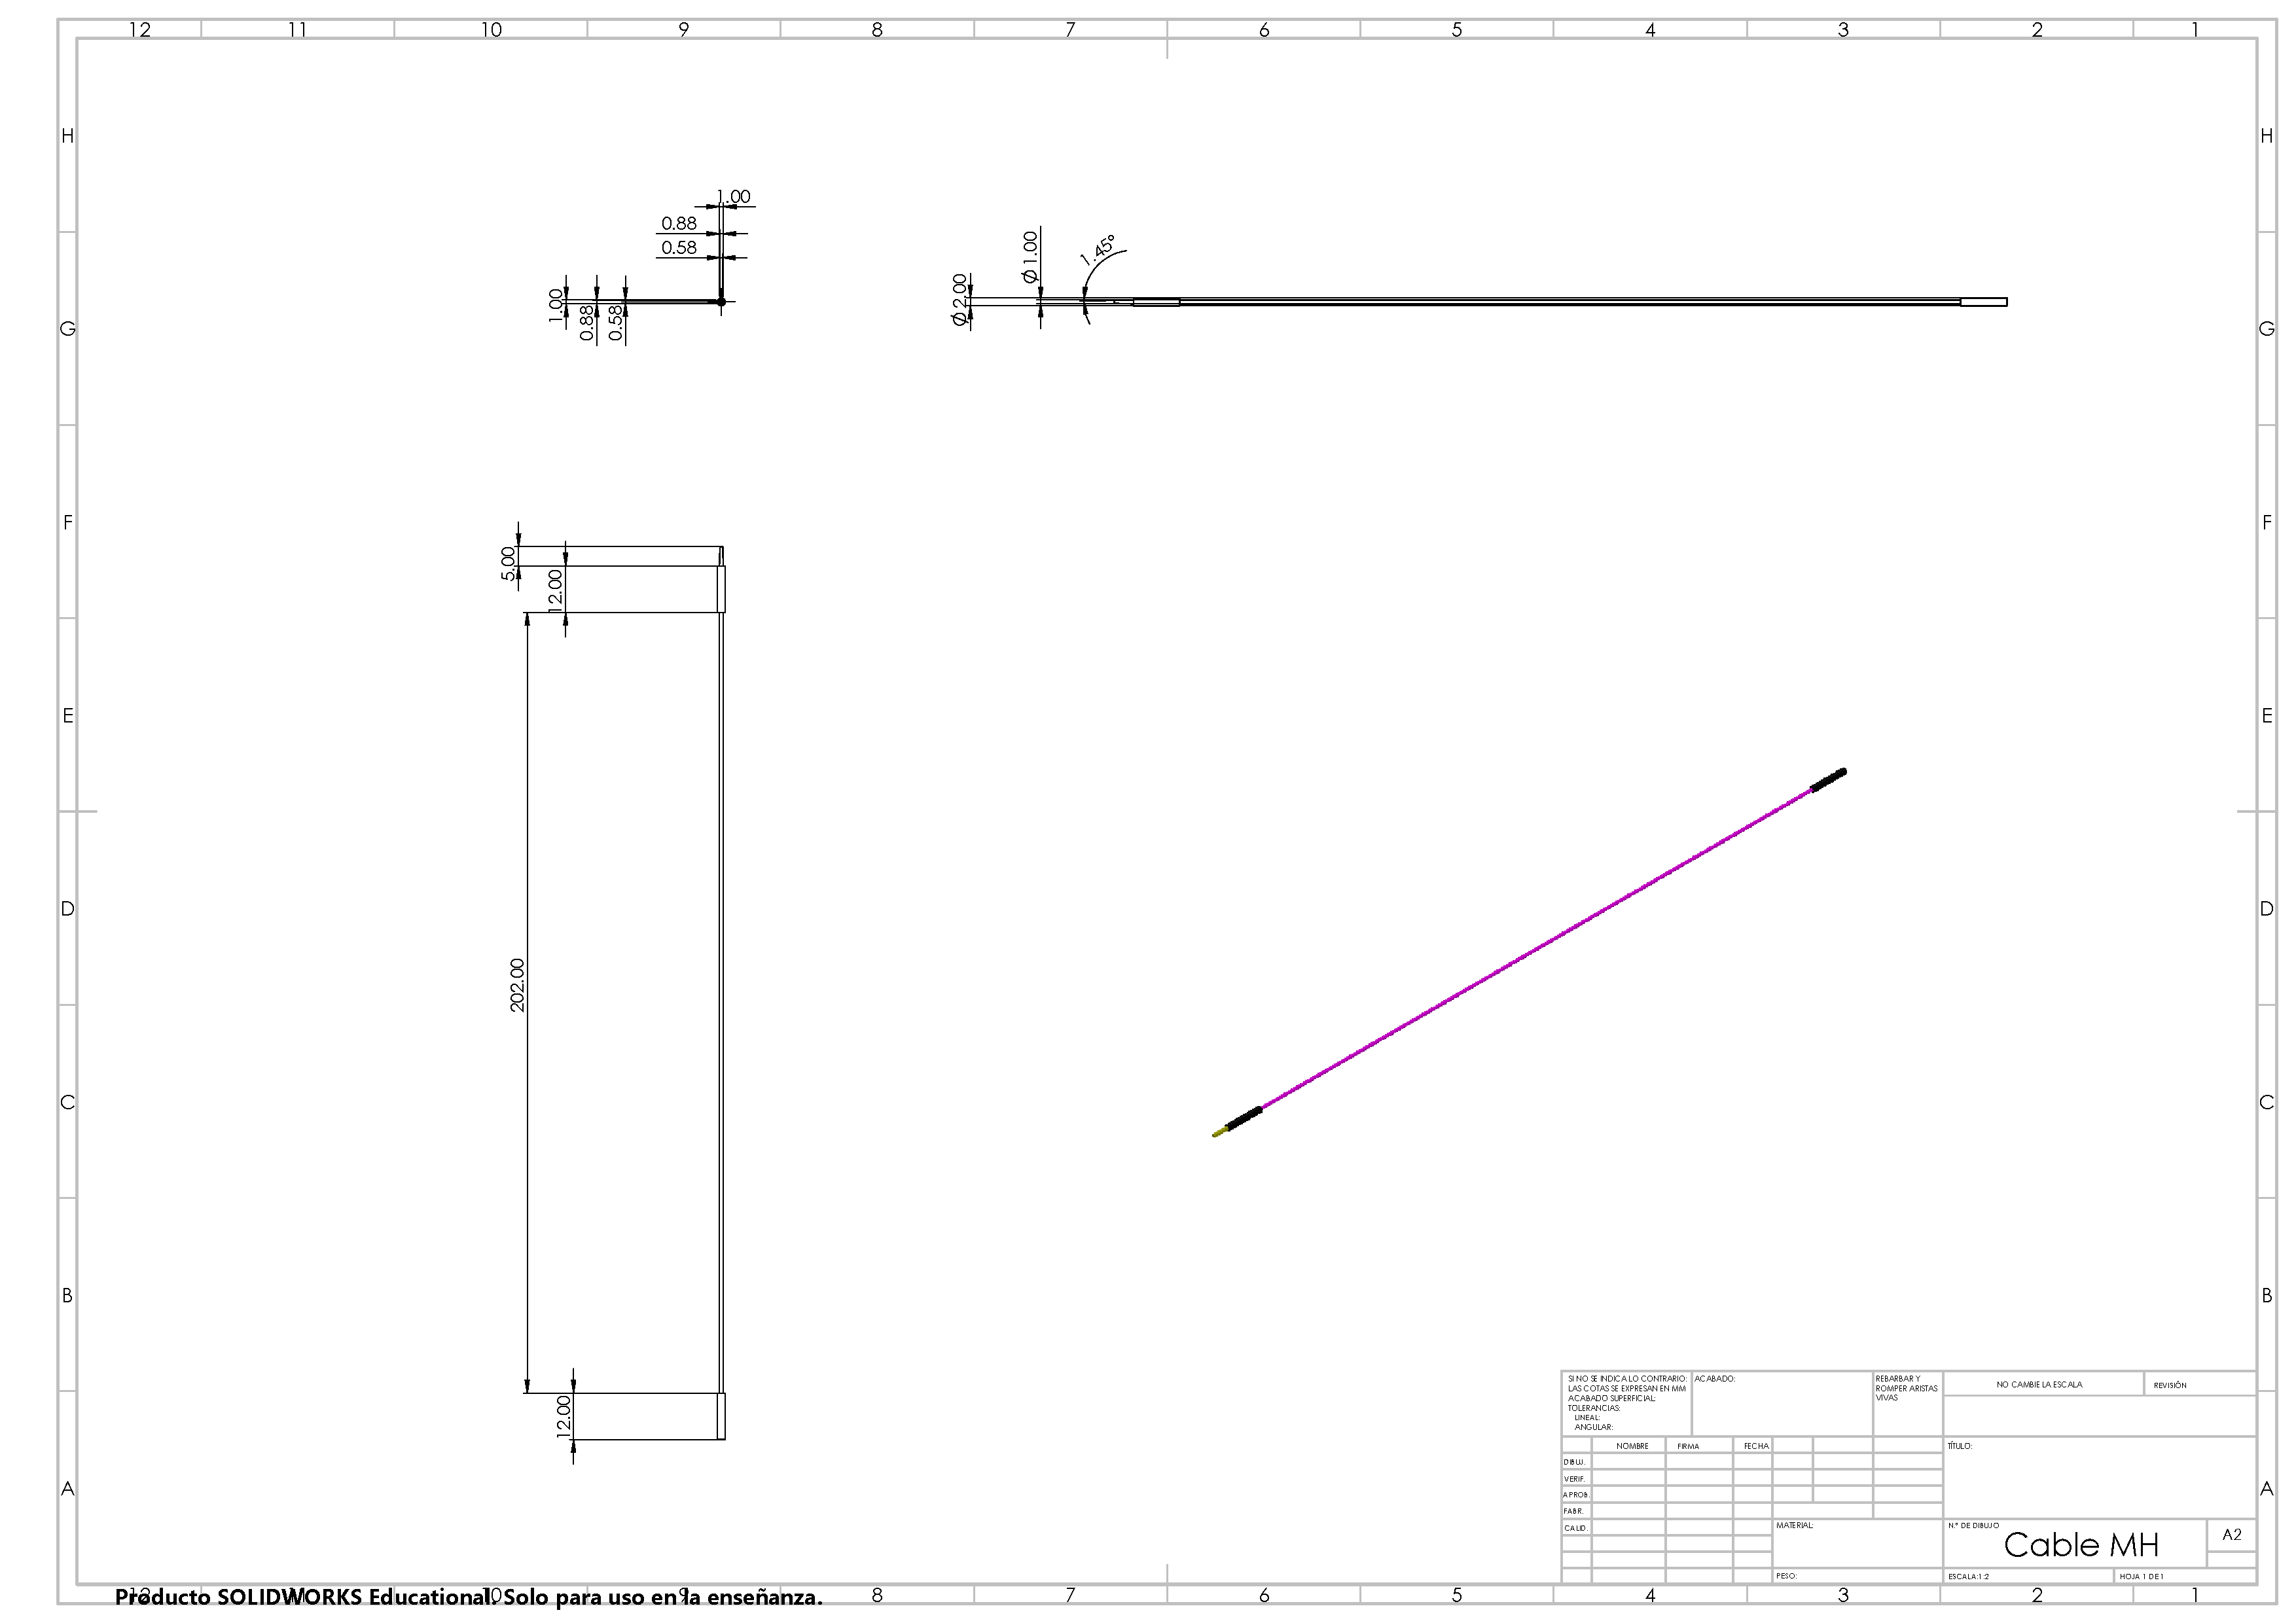
\includegraphics[scale=0.125]{24/Img/cabledeConexionmh.PDF}
        \caption{Cable de conexion MH}
        \label{fig:Cable de conexion MH}
    \end{figure}
    % 
    % 
    \begin{figure}[H]
        \centering
        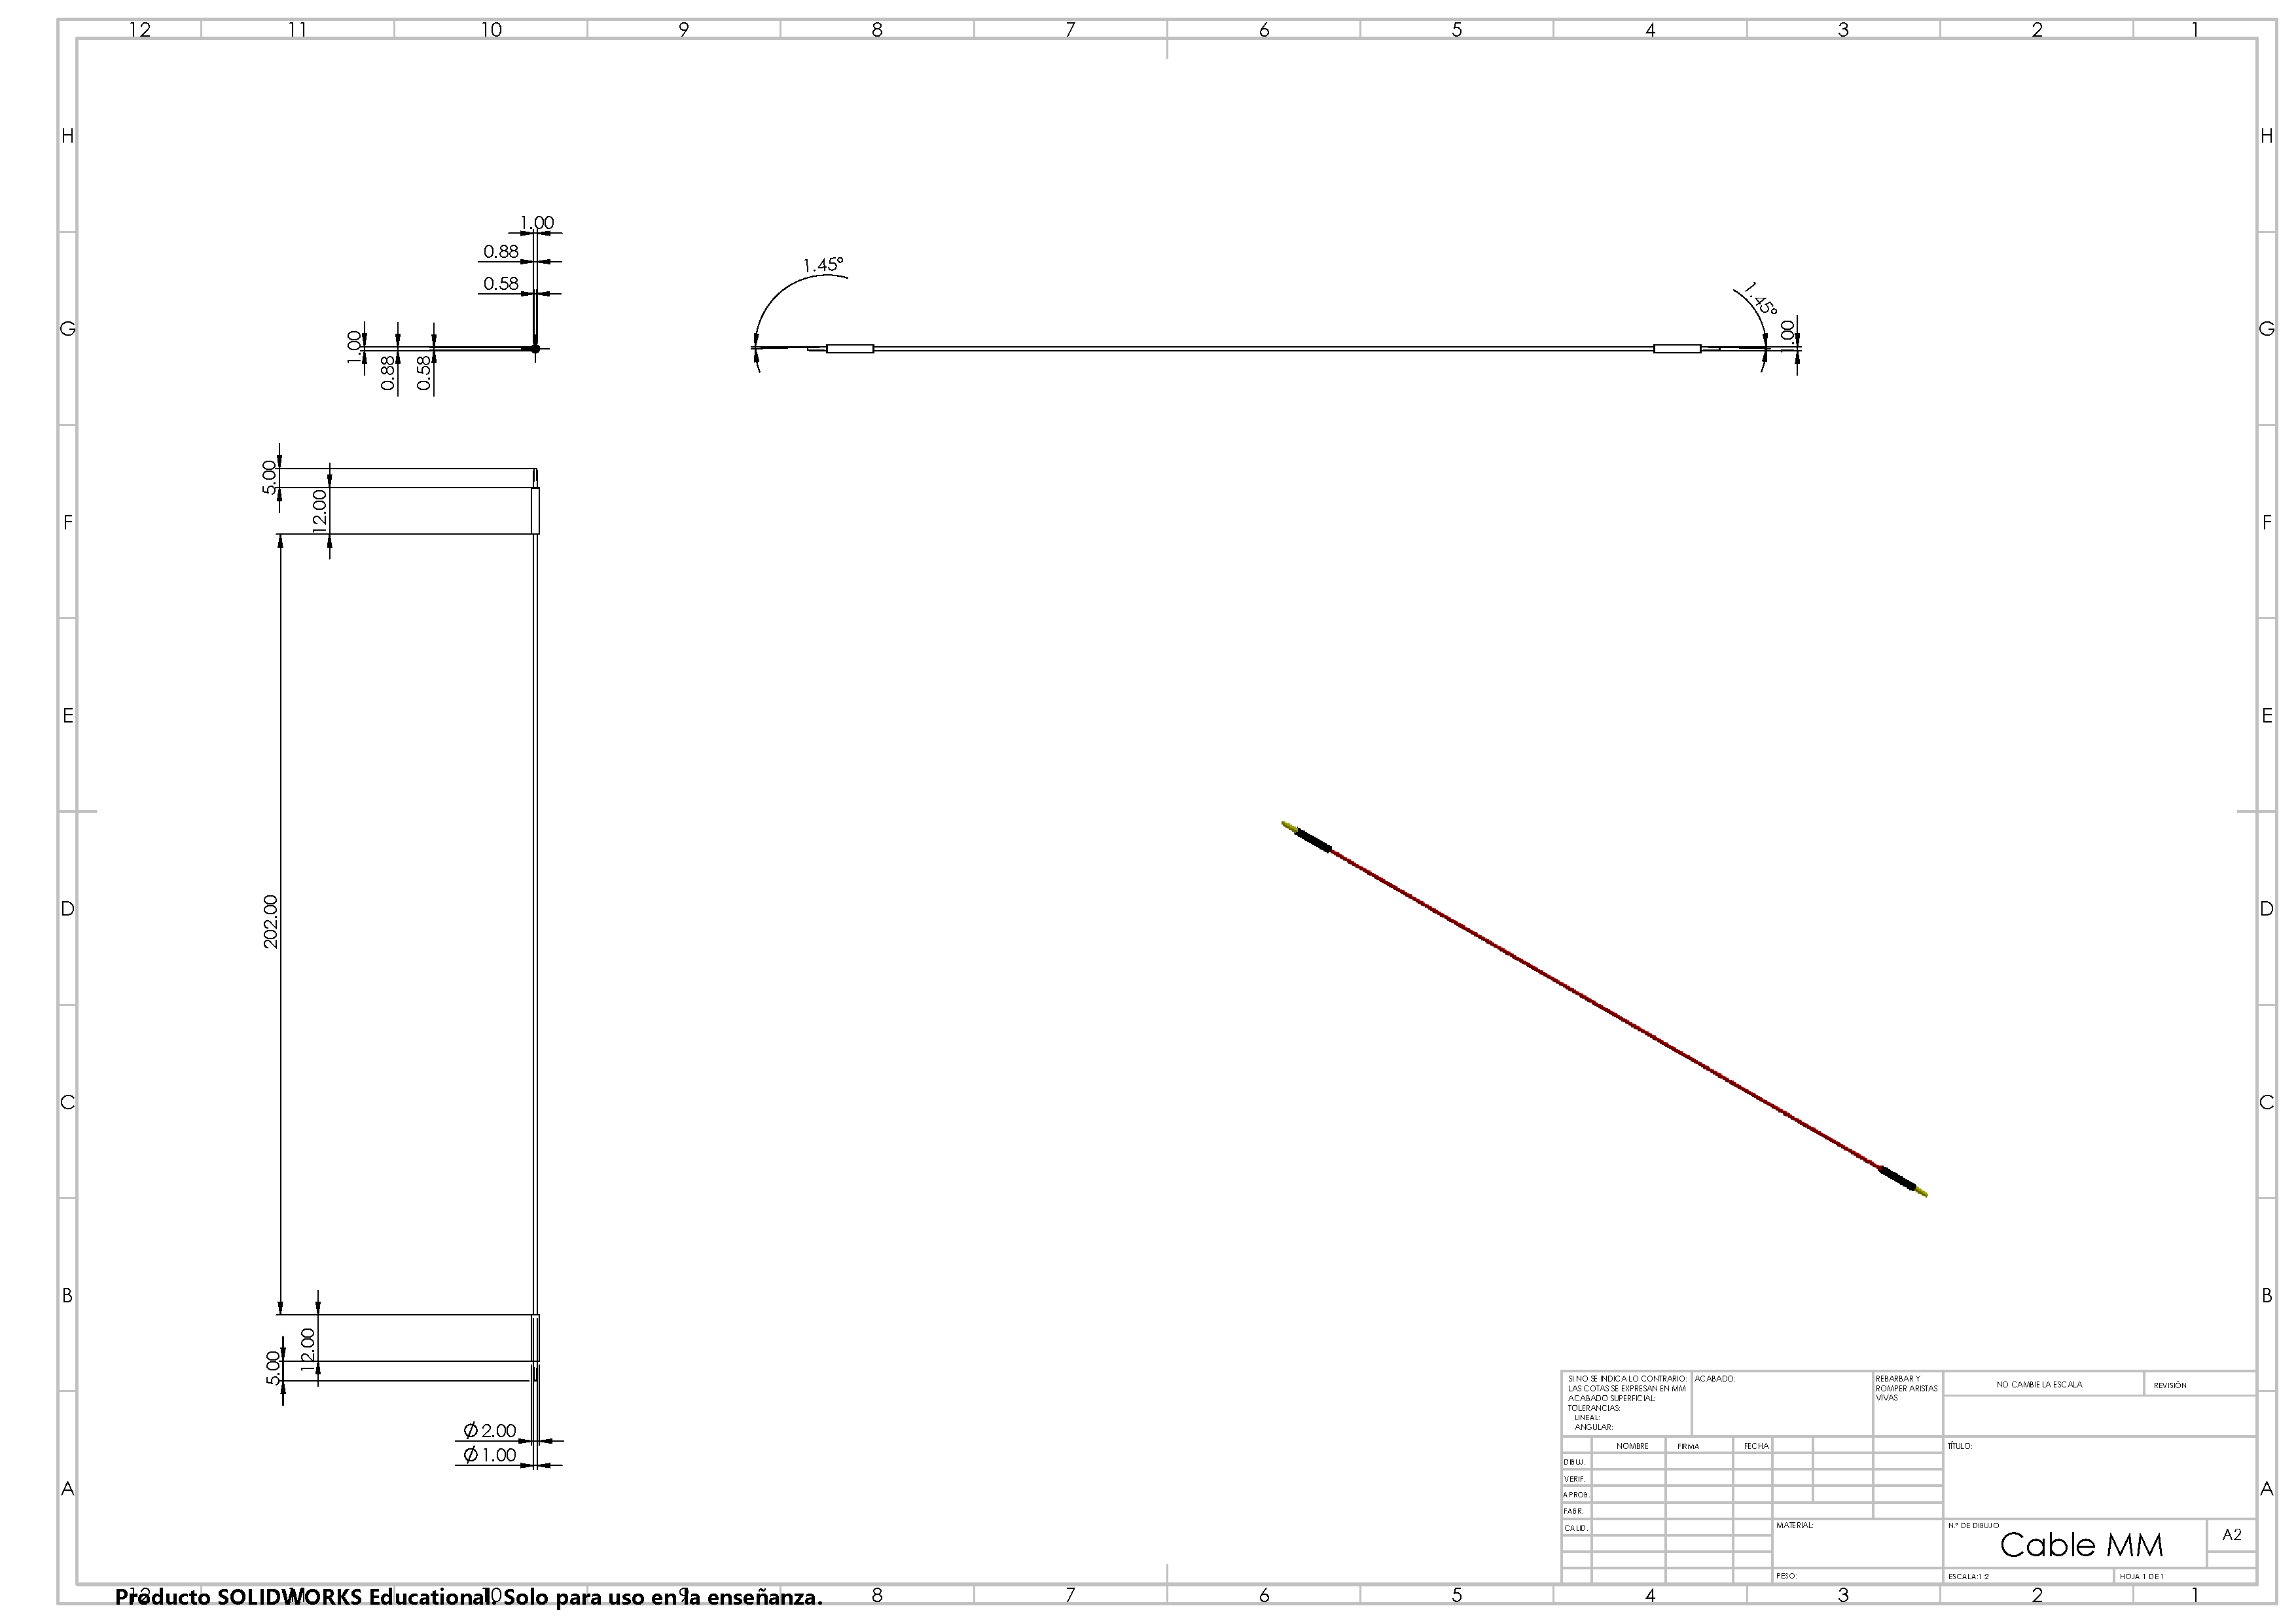
\includegraphics[trim = {10mm 10mm 10mm 10mm},clip,scale=0.120]{24/Img/cabledeConexionmm.pdf}
        \caption{Cable de conexion MM}
        \label{fig:Cable de conexion MM}
    \end{figure}
    % 
    %
    %
    \begin{itemize}
        \item 
        Potenciómetro. Este es un componente electrónico ajustable que permite varear la resistencia en un circuito de forma lineal, con un valor nominal de 1 kiloohmio, este dispositivo ofrece una alta precisión en el control de la resistencia, lo que lo hace ideal para aplicaciones que requieren un ajuste fino, como en controles de volumen, ajuste de señales analógicas y calibración de equipos electrónicos. Véase su respectiva figura\ref{fig:Potenciometro}
    \end{itemize}
    % 
    % 
    \begin{figure}[H]
        \centering
        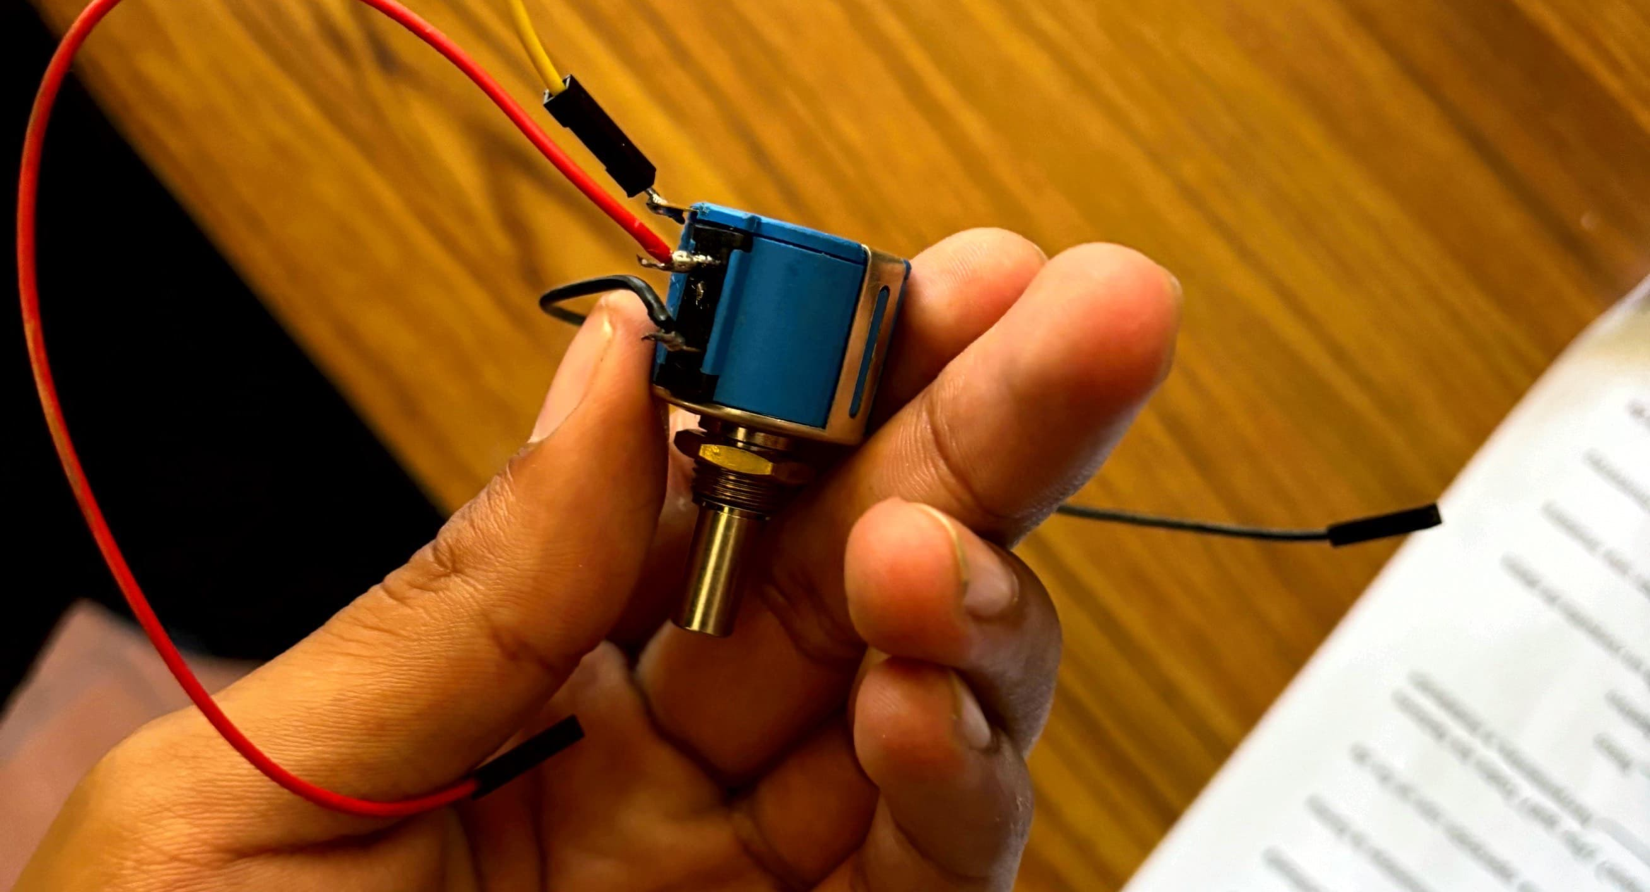
\includegraphics[trim = {10mm 10mm 10mm 10mm},clip,scale=0.120]{24/Img/Potenciometro.pdf}
        \caption{Potenciometro}
        \label{fig:Potenciometro}
    \end{figure}
    % 
    %
    \begin{itemize}
        \item 
        Pantalla LCD 16X2. Es un modulo de visualización que muestra hasta 16 caracteres por linea en dos lineas, sumando un total de 32 caracteres. Es ampliamente utilizada en proyectos de electrónica para presentar información de manera clara y legible. Estas pantallas son eficientes enérgicamente y fáciles de integrar con microcontroladores como Arduino y Raspberry. su interfaz generalmente incluye pines de control y datos, permitiendo la visualización de texto, numero y caracteres personalizados.\ref{fig:LCD 16X2}
    \end{itemize}
    % 
    % 
    \begin{figure}[H]
        \centering
       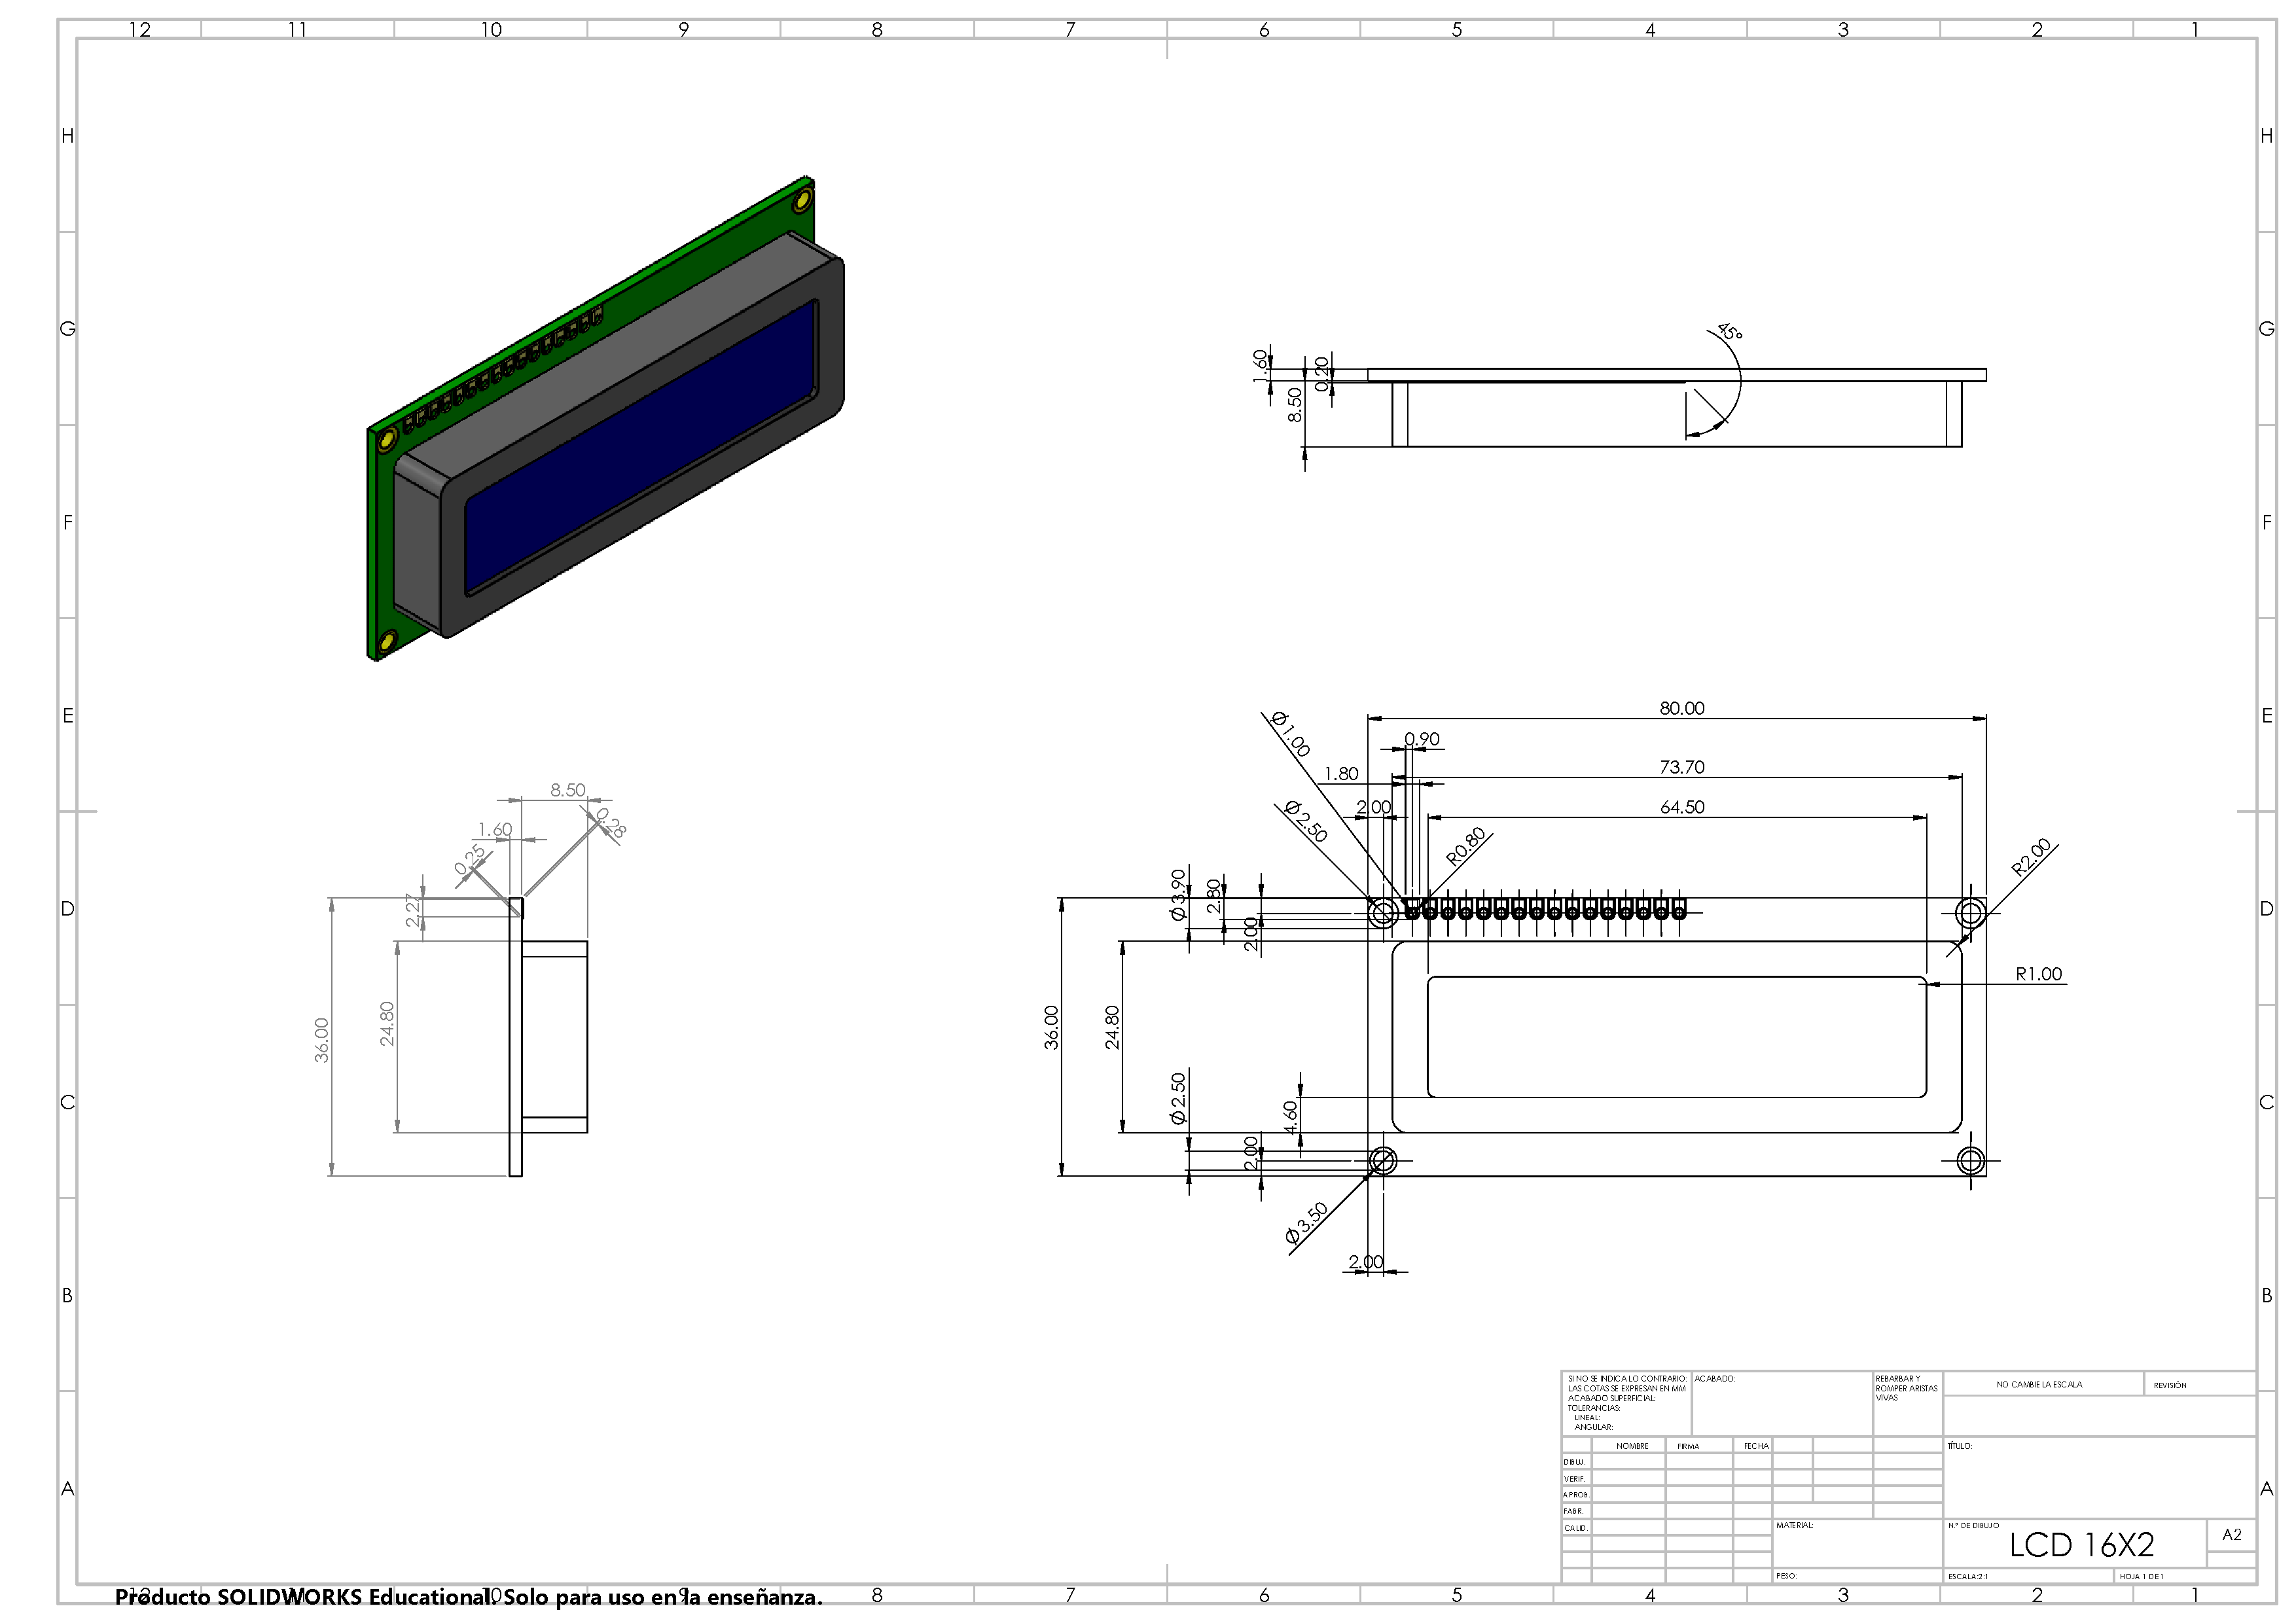
\includegraphics[trim = {10mm 10mm 10mm 10mm},clip,scale=0.120]{24/Img/LCD16X2.pdf}
        \caption{LCD 16X2}
        \label{fig:LCD 16X2}
    \end{figure}
    % 
    %
    \begin{itemize}
        \item 
        Modulo 12C. Es un adaptador que facilita la conexión de una pantalla LCD 16x2 a microcontroladores utilizando el protocolo I2C. Este módulo reduce significativamente la cantidad de pines necesarios para la conexión, utilizando solo dos pines de datos (SDA y SCL). Esto simplifica el cableado y libera pines en el microcontrolador para otras funciones. Es ideal para proyectos con Arduino, Raspberry Pi y otros sistemas embebidos, permitiendo la visualización de texto y datos de manera eficiente y con un menor uso de recursos.\ref{fig:Modulo 12C}
    \end{itemize}
    % 
    \begin{figure}[H]
        \centering
       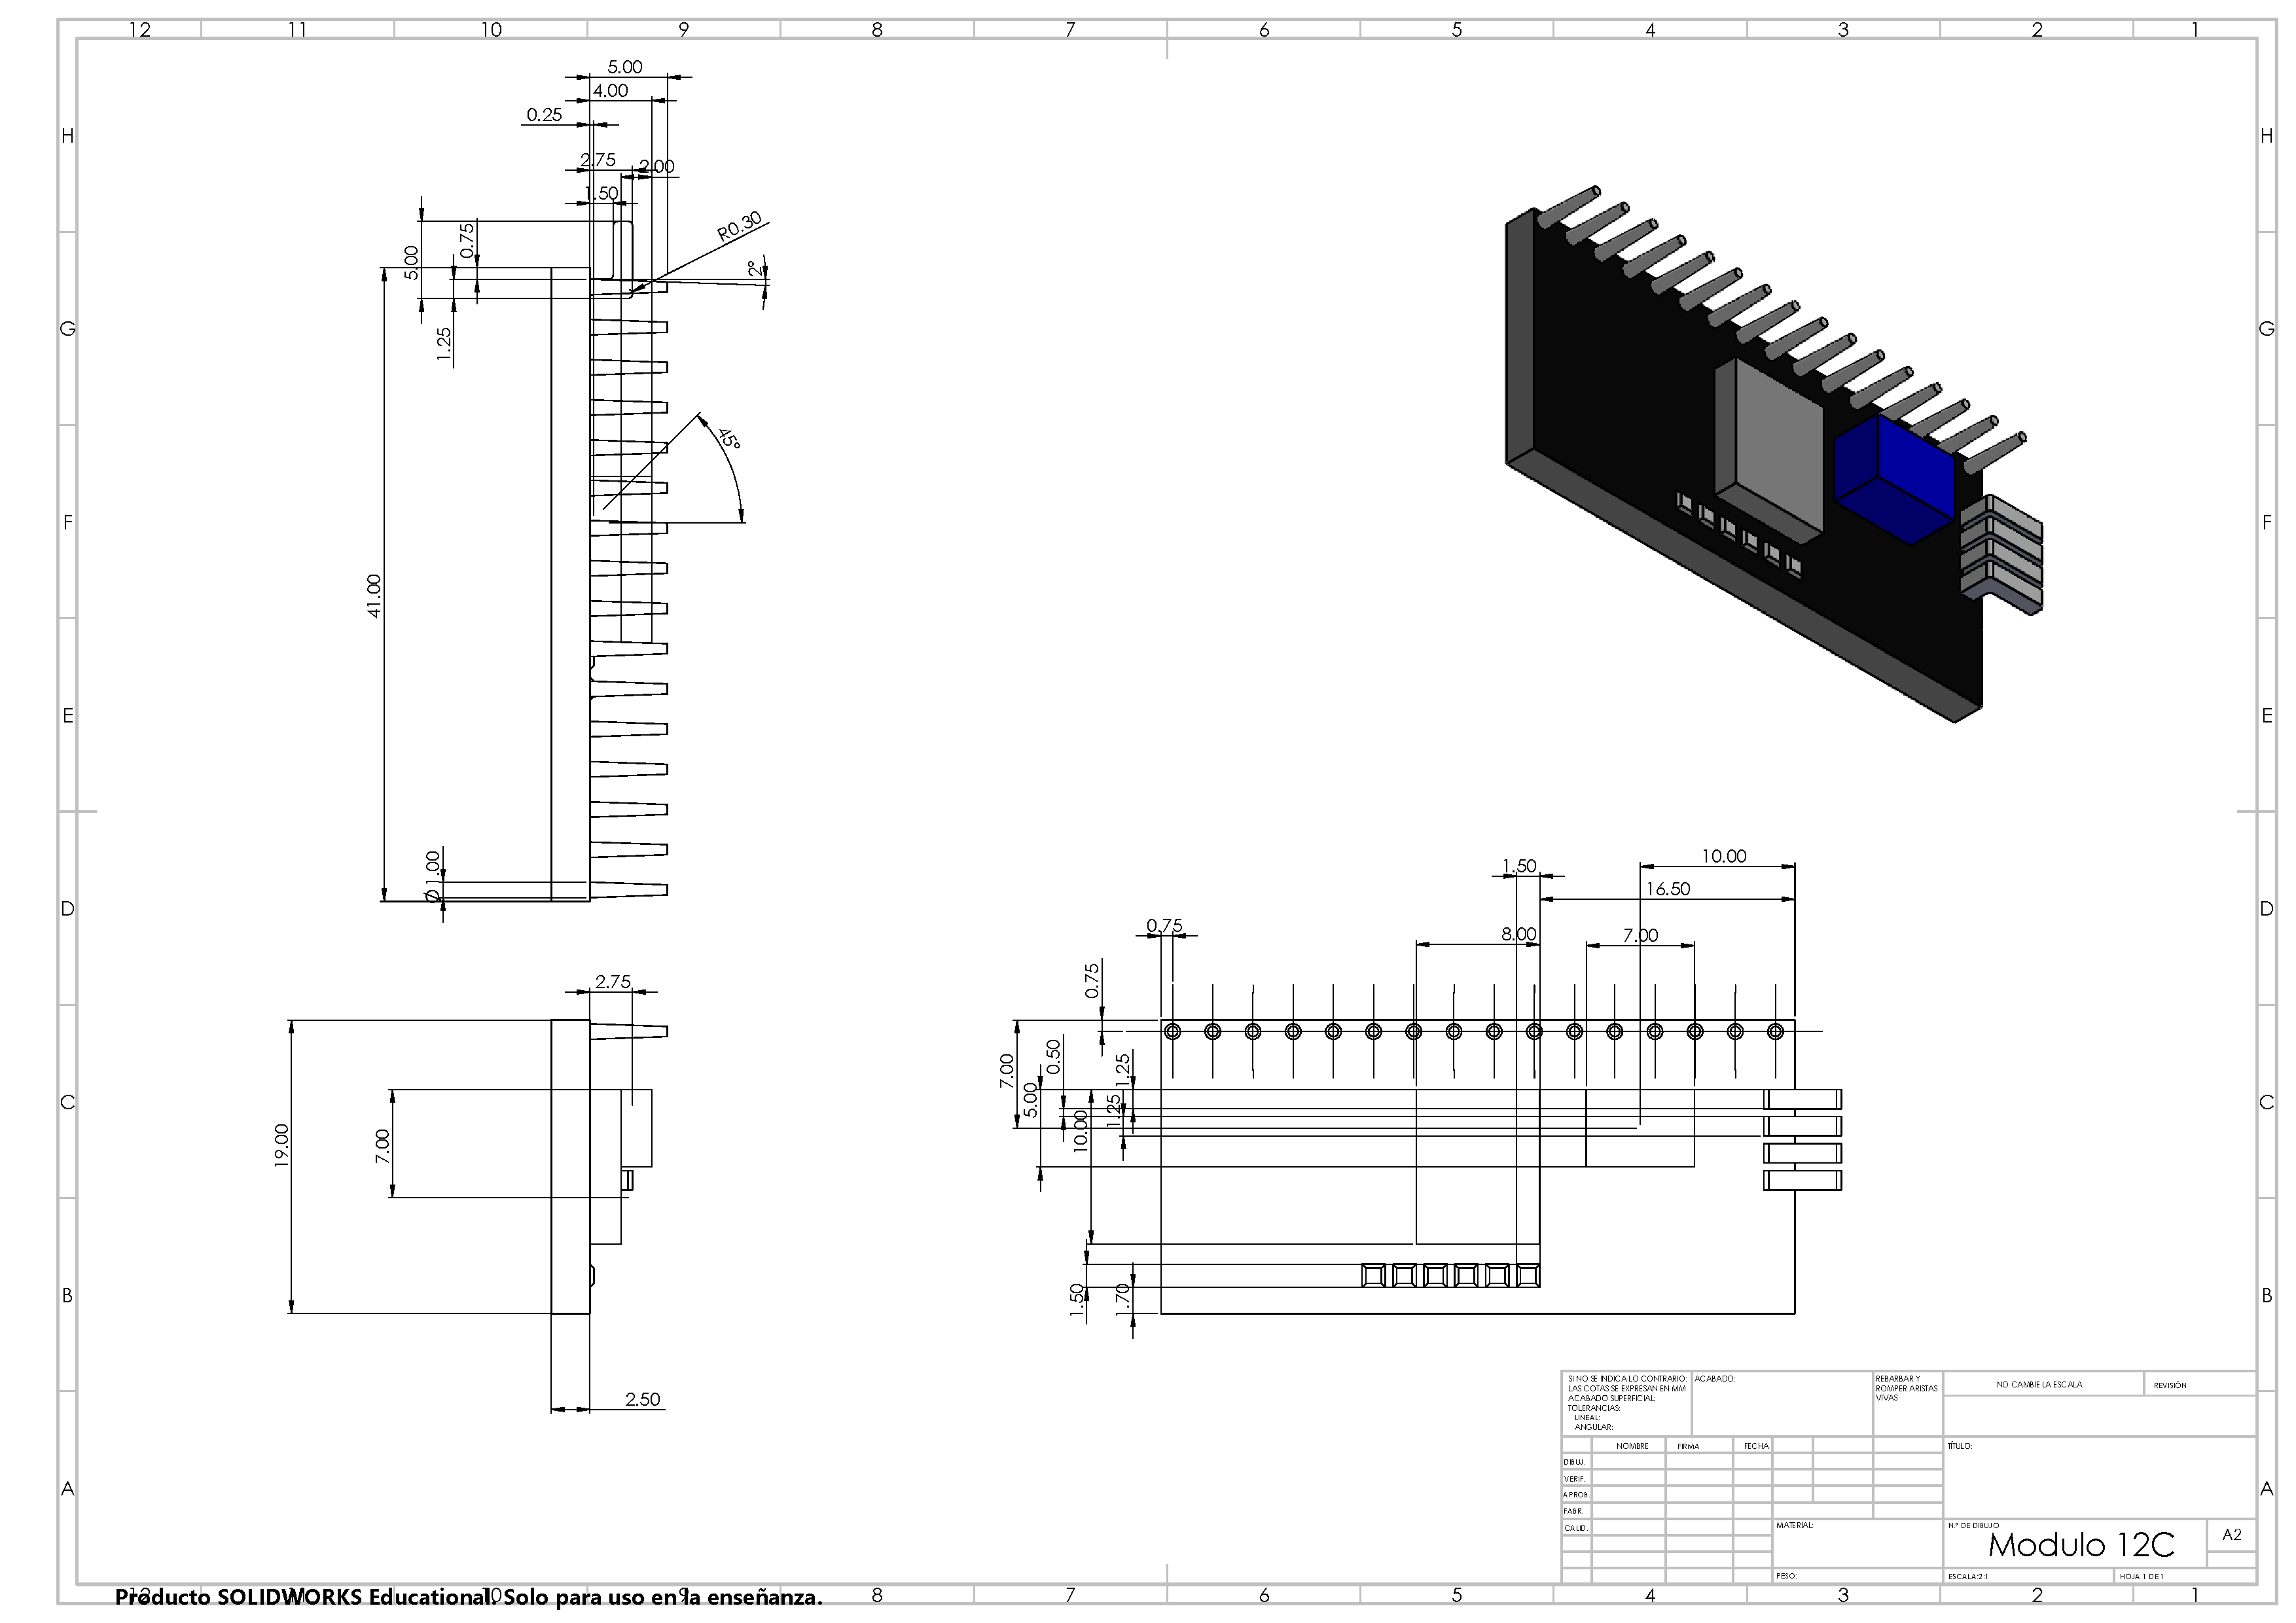
\includegraphics[trim = {10mm 10mm 10mm 10mm},clip,scale=0.120]{24/Img/modulo12C.pdf}
        \caption{Modulo 12C}
        \label{fig:Modulo 12C}
    \end{figure}
    % 
    %
    \begin{itemize}
        \item 
        La ESP 32-C6, Es un modulo de conectividad avanzada que integra Wi-Fi 6, Bluetooth 5 y Zigbee 3.0, ofreciendo una solución versátil para aplicaciones de Internet de las Cosas (IoT). Diseñado por Espressif Systems, este módulo combina alta eficiencia energética y rendimiento, ideal para proyectos que requieren comunicación inalámbrica robusta y de baja latencia. El ESP32-C6-WROOM-1 incluye un potente procesador, múltiples interfaces de E/S y capacidades de seguridad mejoradas, lo que lo convierte en una opción excelente para desarrollos en domótica, dispositivos portátiles y sistemas de automatización industrial.\ref{fig:ESP32}
    \end{itemize}
    % 
    % 
    \begin{figure}[H]
        \centering
        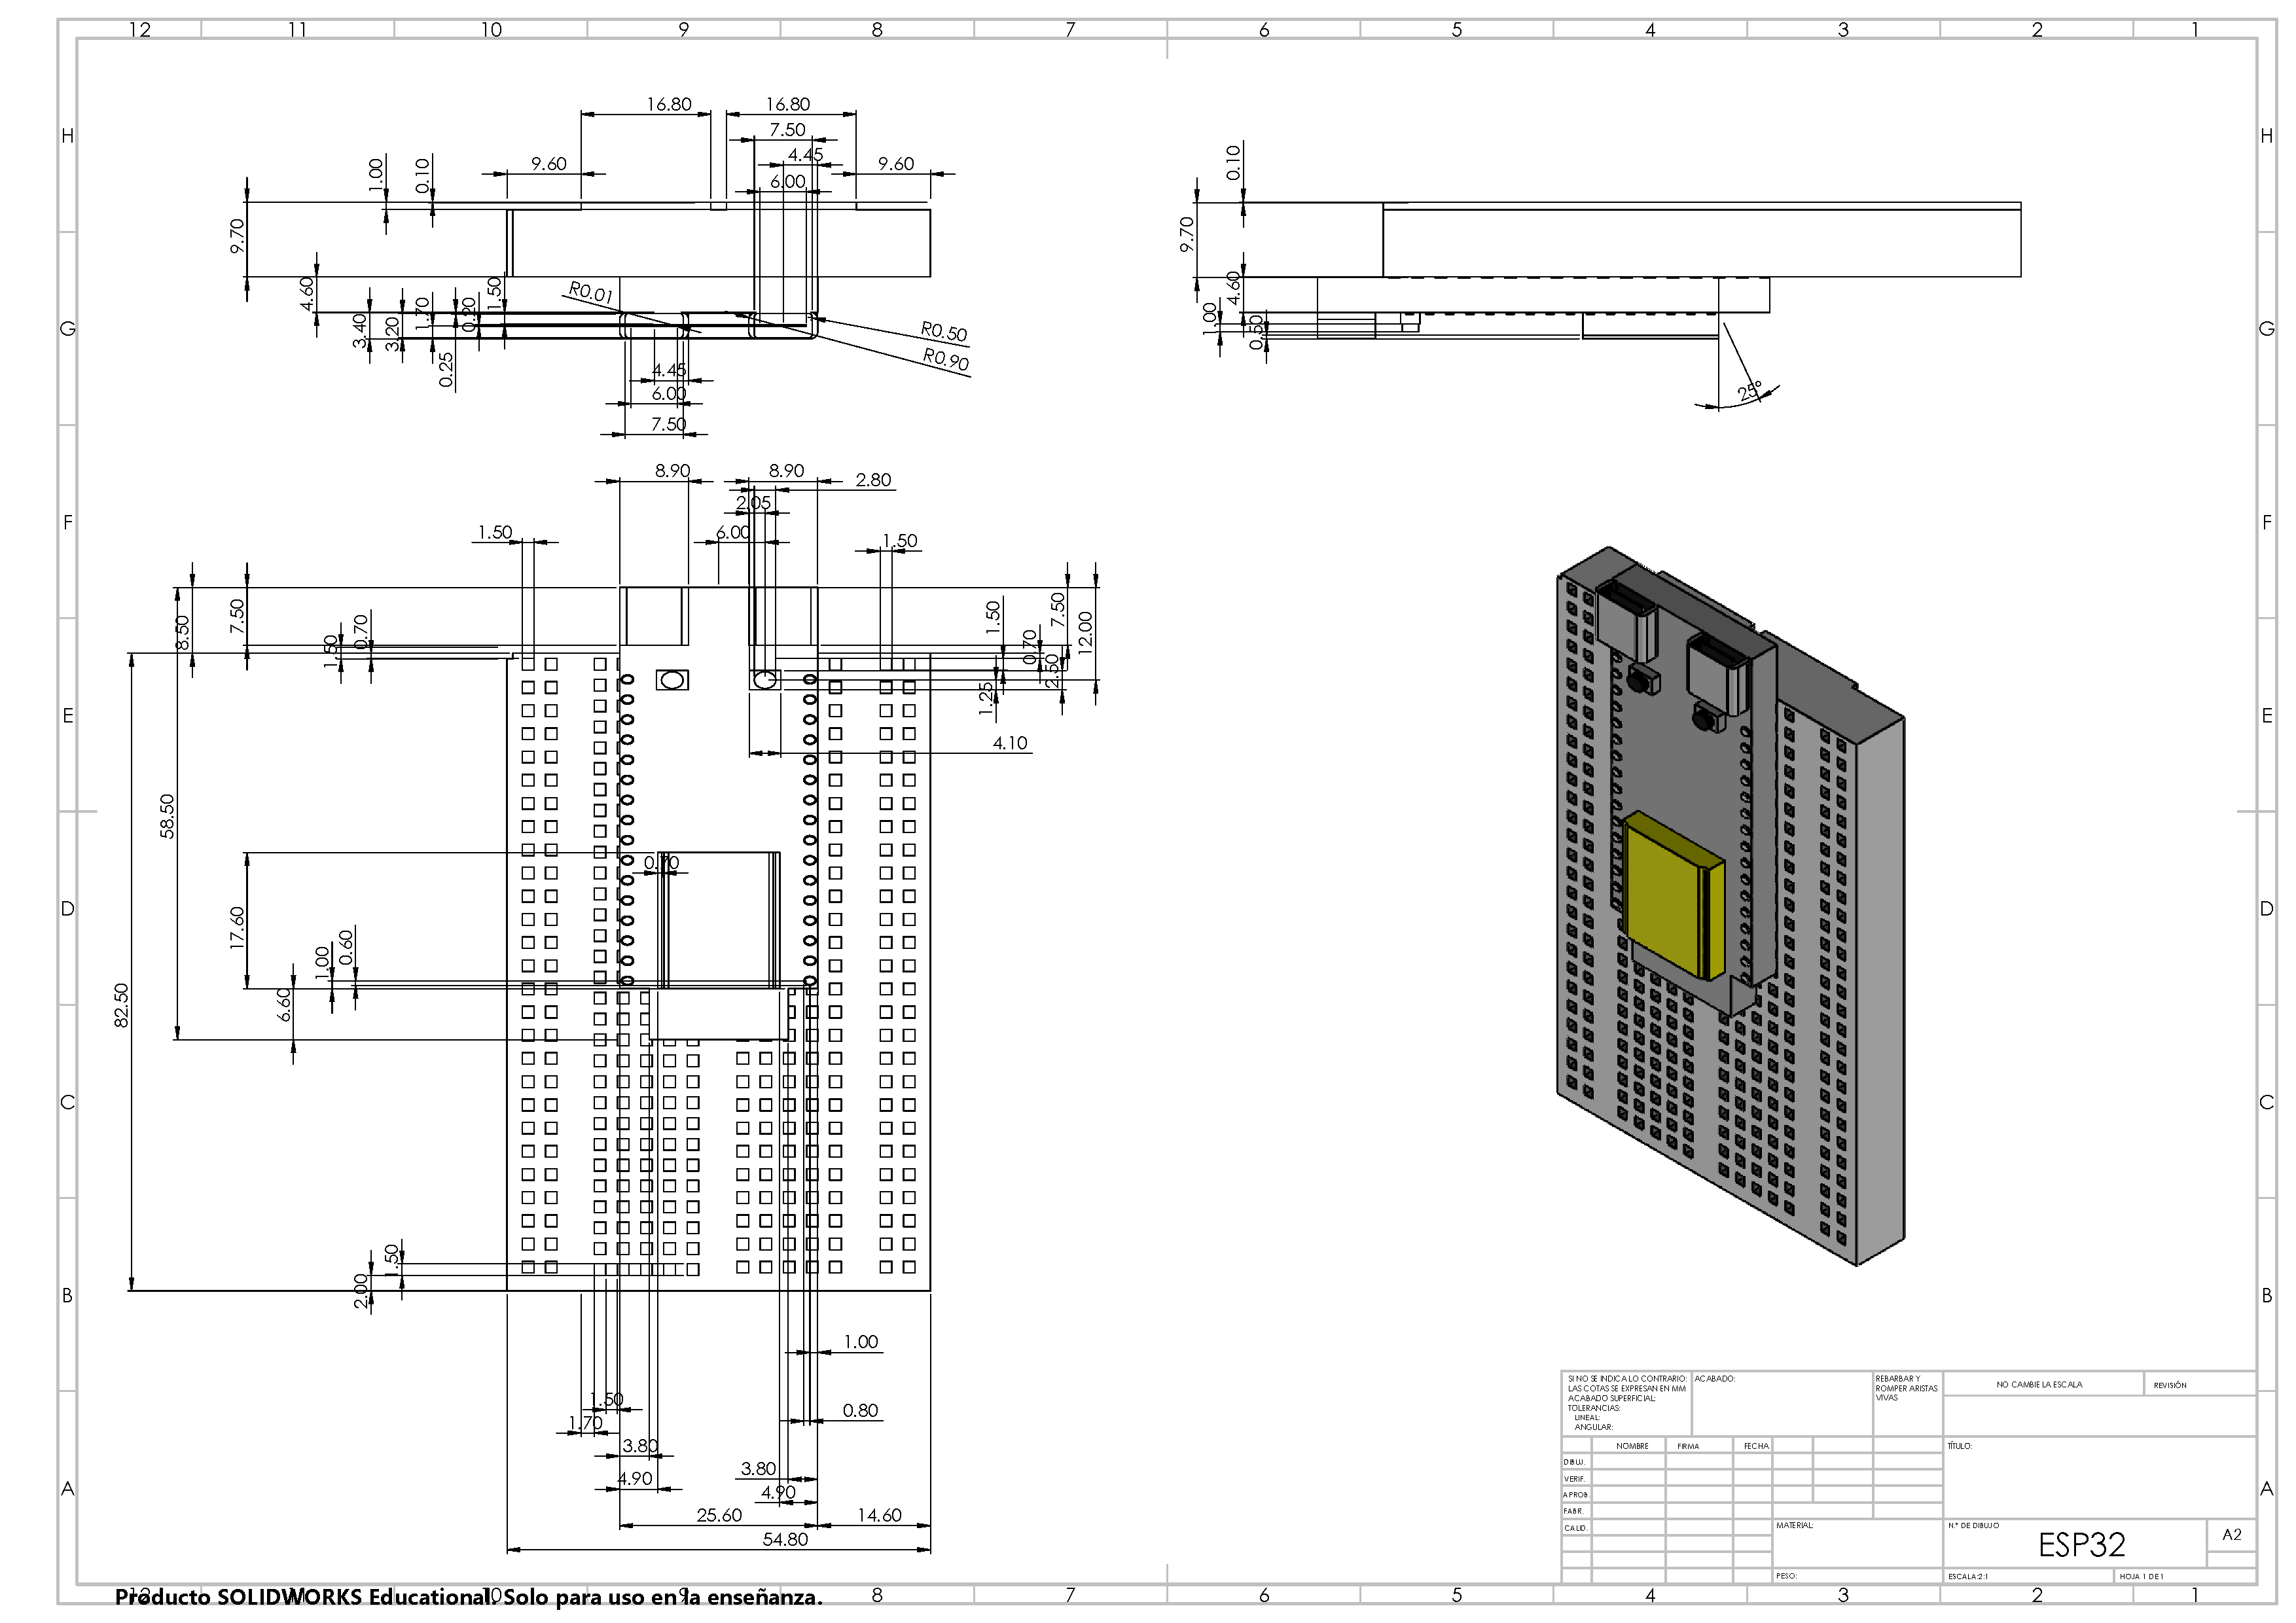
\includegraphics[trim = {10mm 10mm 10mm 10mm},clip,scale=0.120]{24/Img/ESP32.pdf}
        \caption{ESP32}
        \label{fig:ESP32}
    \end{figure}
    % 
    %
    \begin{itemize}
        \item 
        La resistencia de 330 Ohm. Es un componente pasivo utilizado en circuitos electrónicos para limitar la corriente y ajustar los niveles de voltaje. Con un valor de resistencia de 330 ohmios y una capacidad de disipación de potencia de 1/4 de vatio, es ideal para aplicaciones de baja potencia. Esta resistencia se utiliza comúnmente en proyectos de electrónica, incluidos circuitos de iluminación LED, divisores de voltaje, y protección de componentes sensibles. Su tamaño estándar permite una fácil integración en protoboards y placas de circuito impreso (PCB).\ref{fig:Resistencia}
    \end{itemize}
    % 
    % 
    \begin{figure}[H]
        \centering
        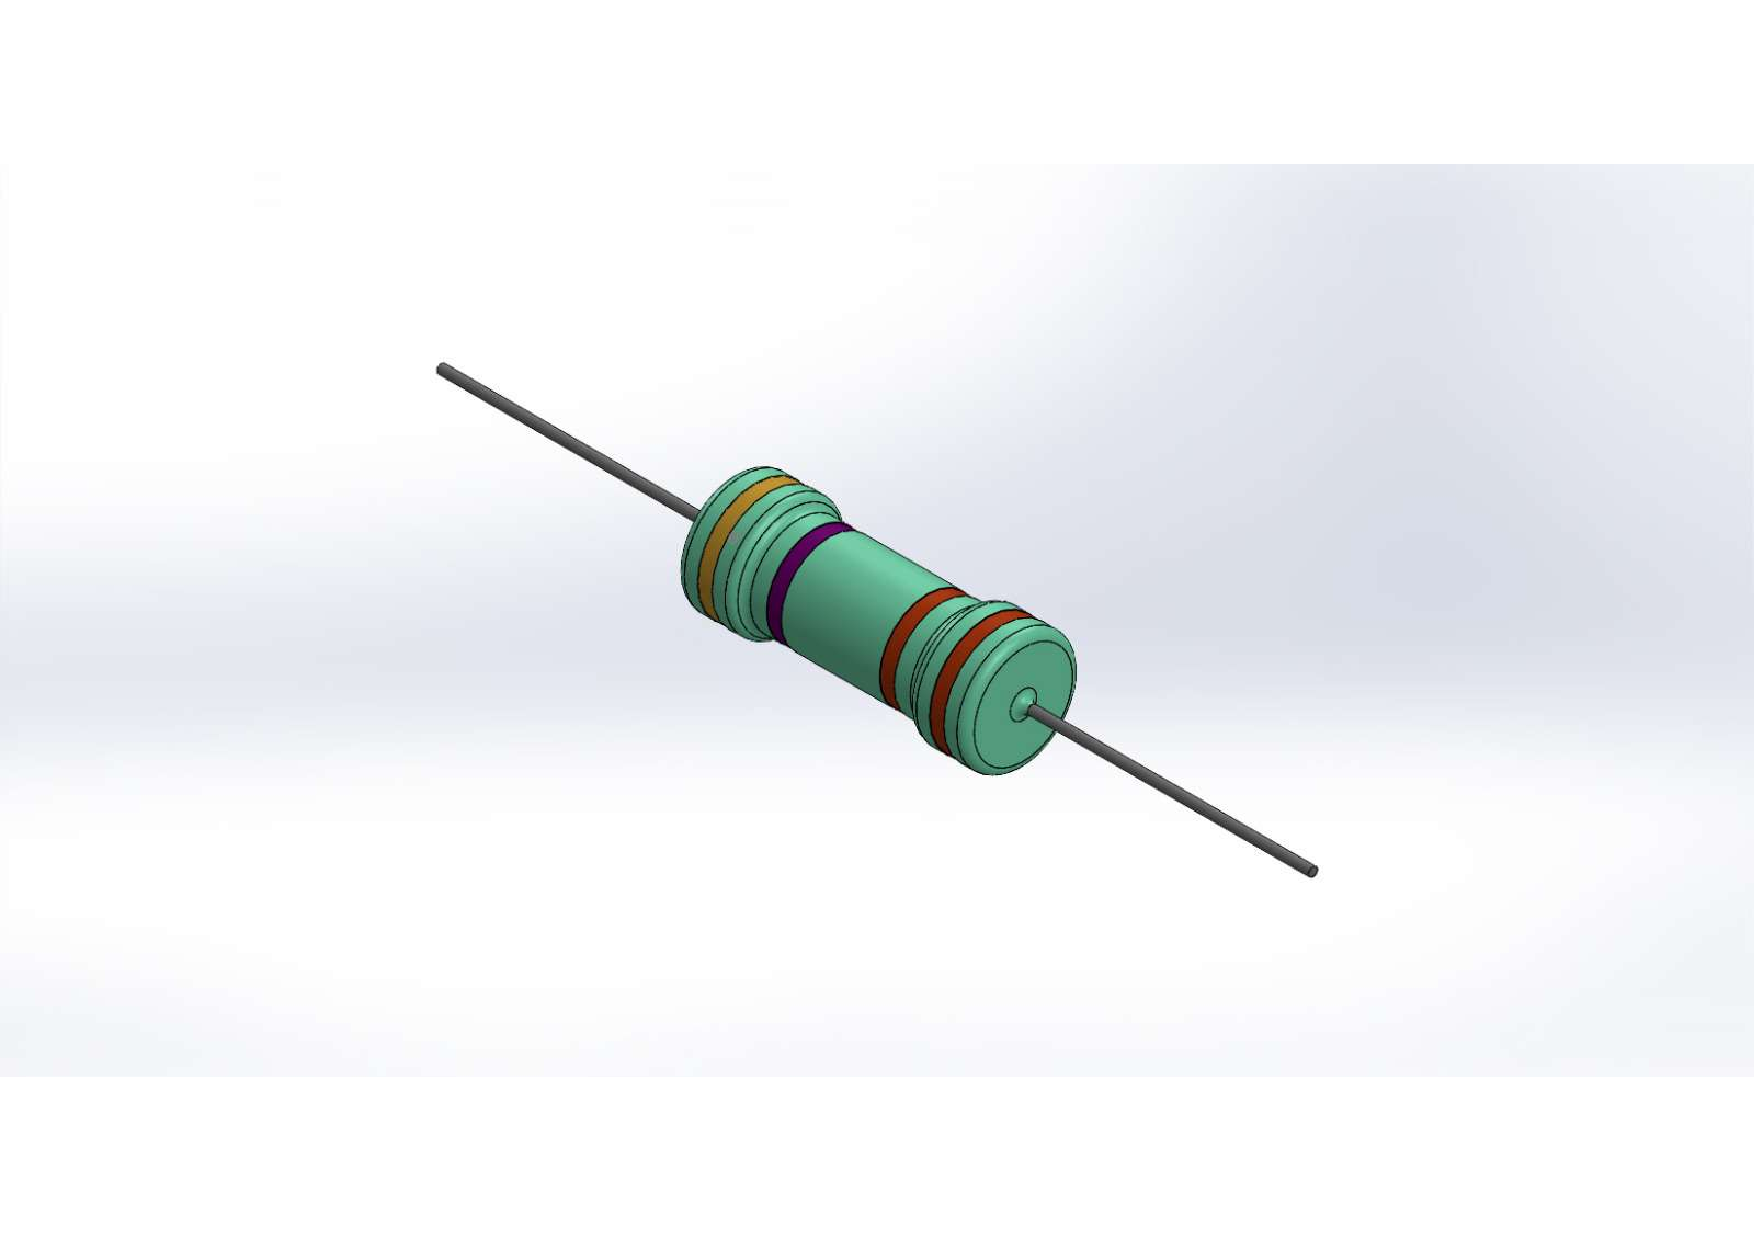
\includegraphics[trim = {10mm 10mm 10mm 10mm},clip,scale=0.120]{24/Img/Resistencia.pdf}
        \caption{Resistencia}
        \label{fig:Resistencia}
    %
    %
    \end{figure}
    % 
    
    %
    %
    Para poder lograr un excelente ensamble y propiciar su buen funcionamiento se elaboro un manual(Véase en las figuras = \ref{fig:enter-label} y \ref{fig:circuitoelectrico}) donde se describe detalladamente cual es cada uno de los movimientos que debe realizar el operador para obtener el ensamble exacto. Una vez concluido nuestro manual, continuamos tomando dos muestras continuas con ayuda de nuestro teléfono móvil, donde el operador se guió del manual antes mencionado, realizándolo en distintos días, a distinta hora y en distinto lugar, donde además evitábamos tener el mínimo contacto con nuestro operador para no causar interrupciones, ni retardos en el trabajo, se implementaron las 5s y además debemos culminar con un análisis de costos para determinar el cuarto factor, el cual ayuda a obtener la eficiencia y la manera mas económica de realizar el trabajo.
    % 
    % 
    \begin{figure}
        \centering
     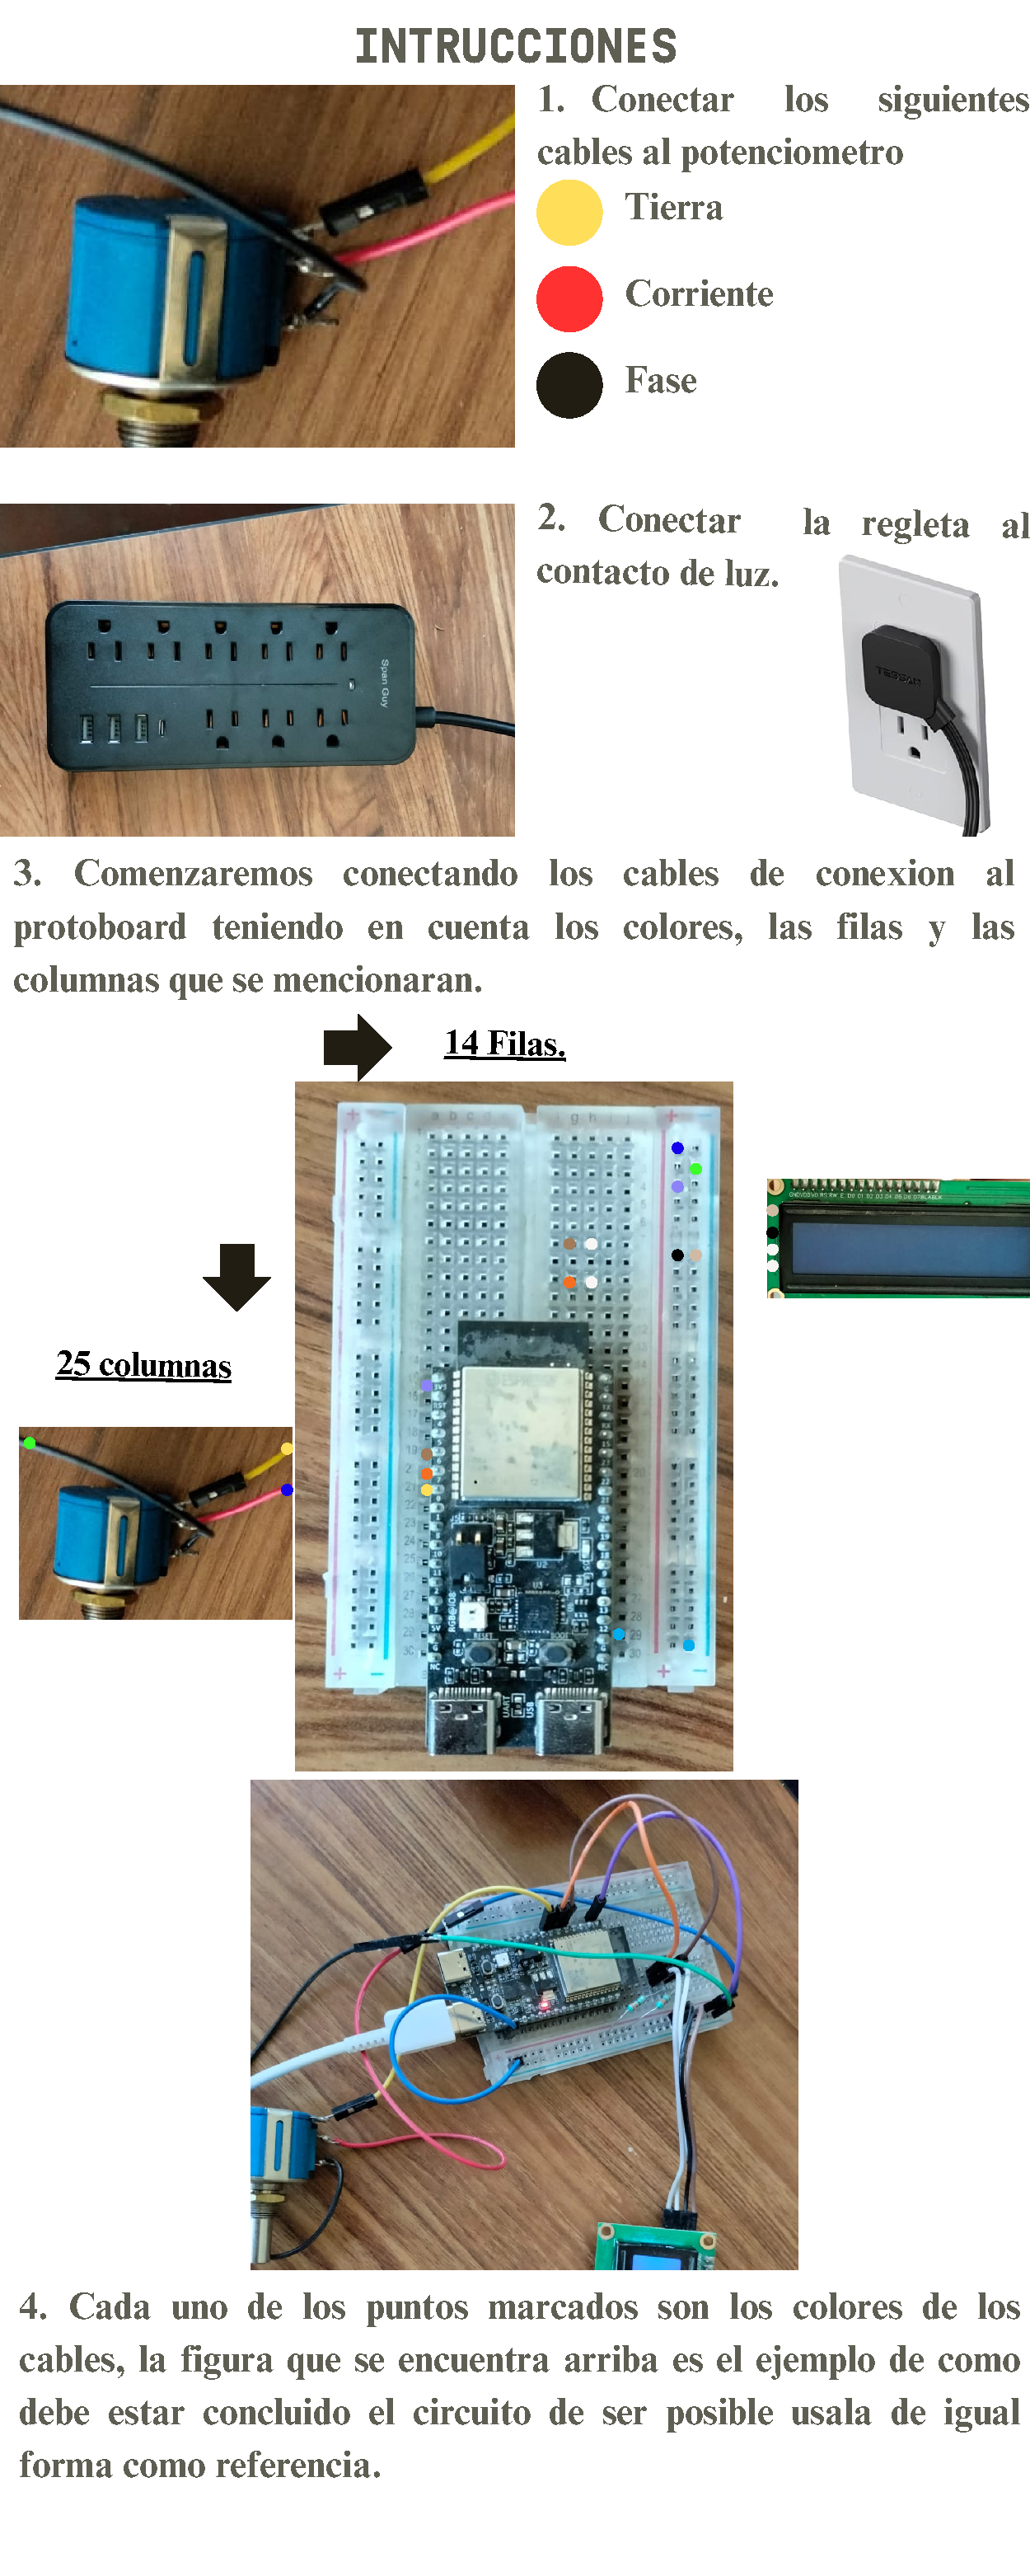
\includegraphics[scale=0.150]{24/Img/circuitoElectricoinstructivo.pdf}
        \caption{Ensamble circuito}
        \label{fig:enter-label}
    \end{figure}
    \begin{figure}
        \centering
    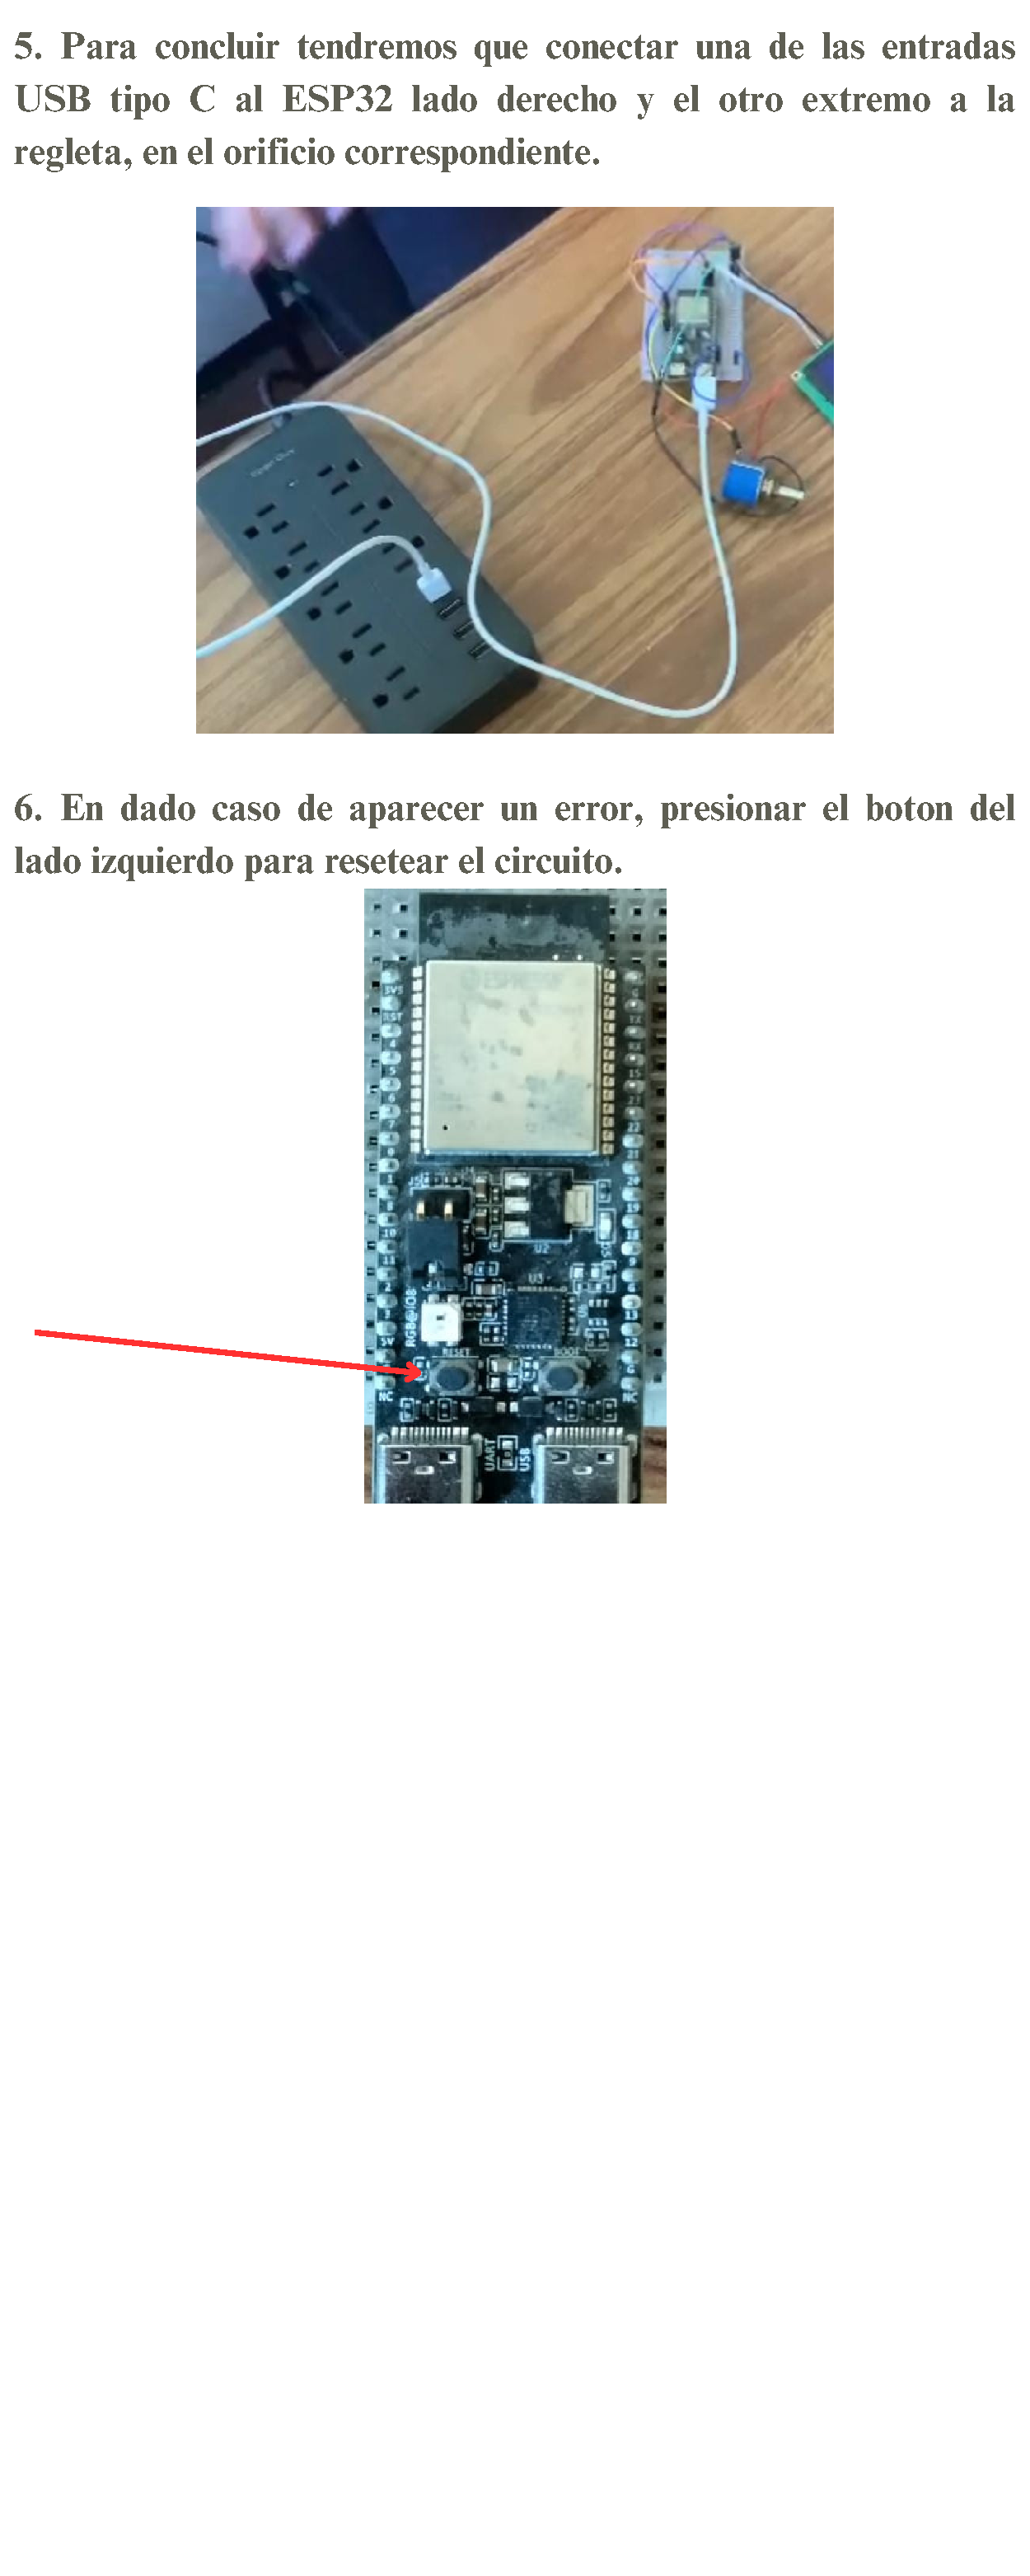
\includegraphics[trim = {20mm 100mm 20mm 0mm},clip,scale=0.150]{24/Img/circuitoElectricoinstructivo2.pdf}
        \caption{Ensamble circuito}
        \label{fig:circuitoelectrico}
    \end{figure}
    %
    %
    %
    \subsubsection{5's}
    La implementación de las 5S en nuestro proceso de ensamblaje es crucial para mantener un entorno de trabajo limpio, organizado y eficiente. Esto no solo mejorará la eficiencia, sino que también aumentará la seguridad y la calidad de nuestro producto final. A continuación, se detalla cómo aplicamos esta metodología. 
    %
    \begin{enumerate}
        \item Clasificación(Seiri): Se identificaran todos los componentes y herramientas necesarios para el ensamblaje del circuito eléctrico. Se deben eliminar todos los elementos innecesarios, incluyendo componentes defectuosos y herramientas irrelevantes. 
        \item Orden(Seiton): Los componentes y herramientas se colocaran en lugares designados y etiquetados, de manera que sea mas fácil el acceder a ellos, reduciendo el tiempo de búsqueda.
        \item Limpieza(Seiso): Se mantendrá el área de trabajo limpia mediante la eliminación de desechos y la limpieza regular de las herramientas y equipos. Esto evitará acumulaciones de suciedad que puedan interferir con el proceso de ensamblaje.
        \item Estandarización(Seiketsu): Se desarrollarán procedimientos estandarizados para la clasificación, organización y limpieza. Se crearán listas de verificación y se realizarán correcciones pertinentes en el manual de procedimientos para asegurar la coherencia en el proceso.
        \item Disciplina(Shitsuke): Se capacitará y motivará al personal para que siga los procedimientos establecidos, realizando supervisiones regulares para asegurar el cumplimiento y mantener la disciplina en el área de trabajo.
    \end{enumerate}
    %
    
    \subsubsection{Desarrollo del sistema de tiempos predeterminados}
    Para conseguir un buen desarrollo en el STP se debe seguir una serie de pasos basados en los Therbligs, estos deben ser aplicados por un analista capaz de comprender y llevarlos a la practica, esto tiene como finalidad realizar un análisis atravesé de la descomposición de cada uno de los movimientos con los que se llevan a cabo el ensamble, en las imágenes \ref{fig:Mover}, \ref{fig:Alcanzar}, \ref{fig:COLOCAR}, \ref{fig:SOLTAR}, se puede mostrar un poco del como se subdivide cada una de ellas, al concluir la clasificación se debe realizar una suma de todos los movimientos. 
    %
    %
    \begin{figure}
        \centering
        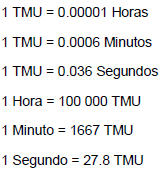
\includegraphics[trim = {0mm 00mm 0mm 0mm},clip,scale=0.5]{24/Img/unidadesdeMedida(MTM).png}
        \caption{UNIDADES DE MEDIDA}
        \label{fig:Unidades}
    \end{figure}
    %
    % 
    \begin{figure}
        \centering
        
\includegraphics[trim = {0mm 00mm 0mm 15mm},clip,scale=0.3]{24/Img/tablaAlcanzar.pdf}
        \caption{TABLA- ALCANZAR}
        \label{fig:Alcanzar}
    \end{figure}
    %
    % 
    %
    \begin{figure}
        \centering
        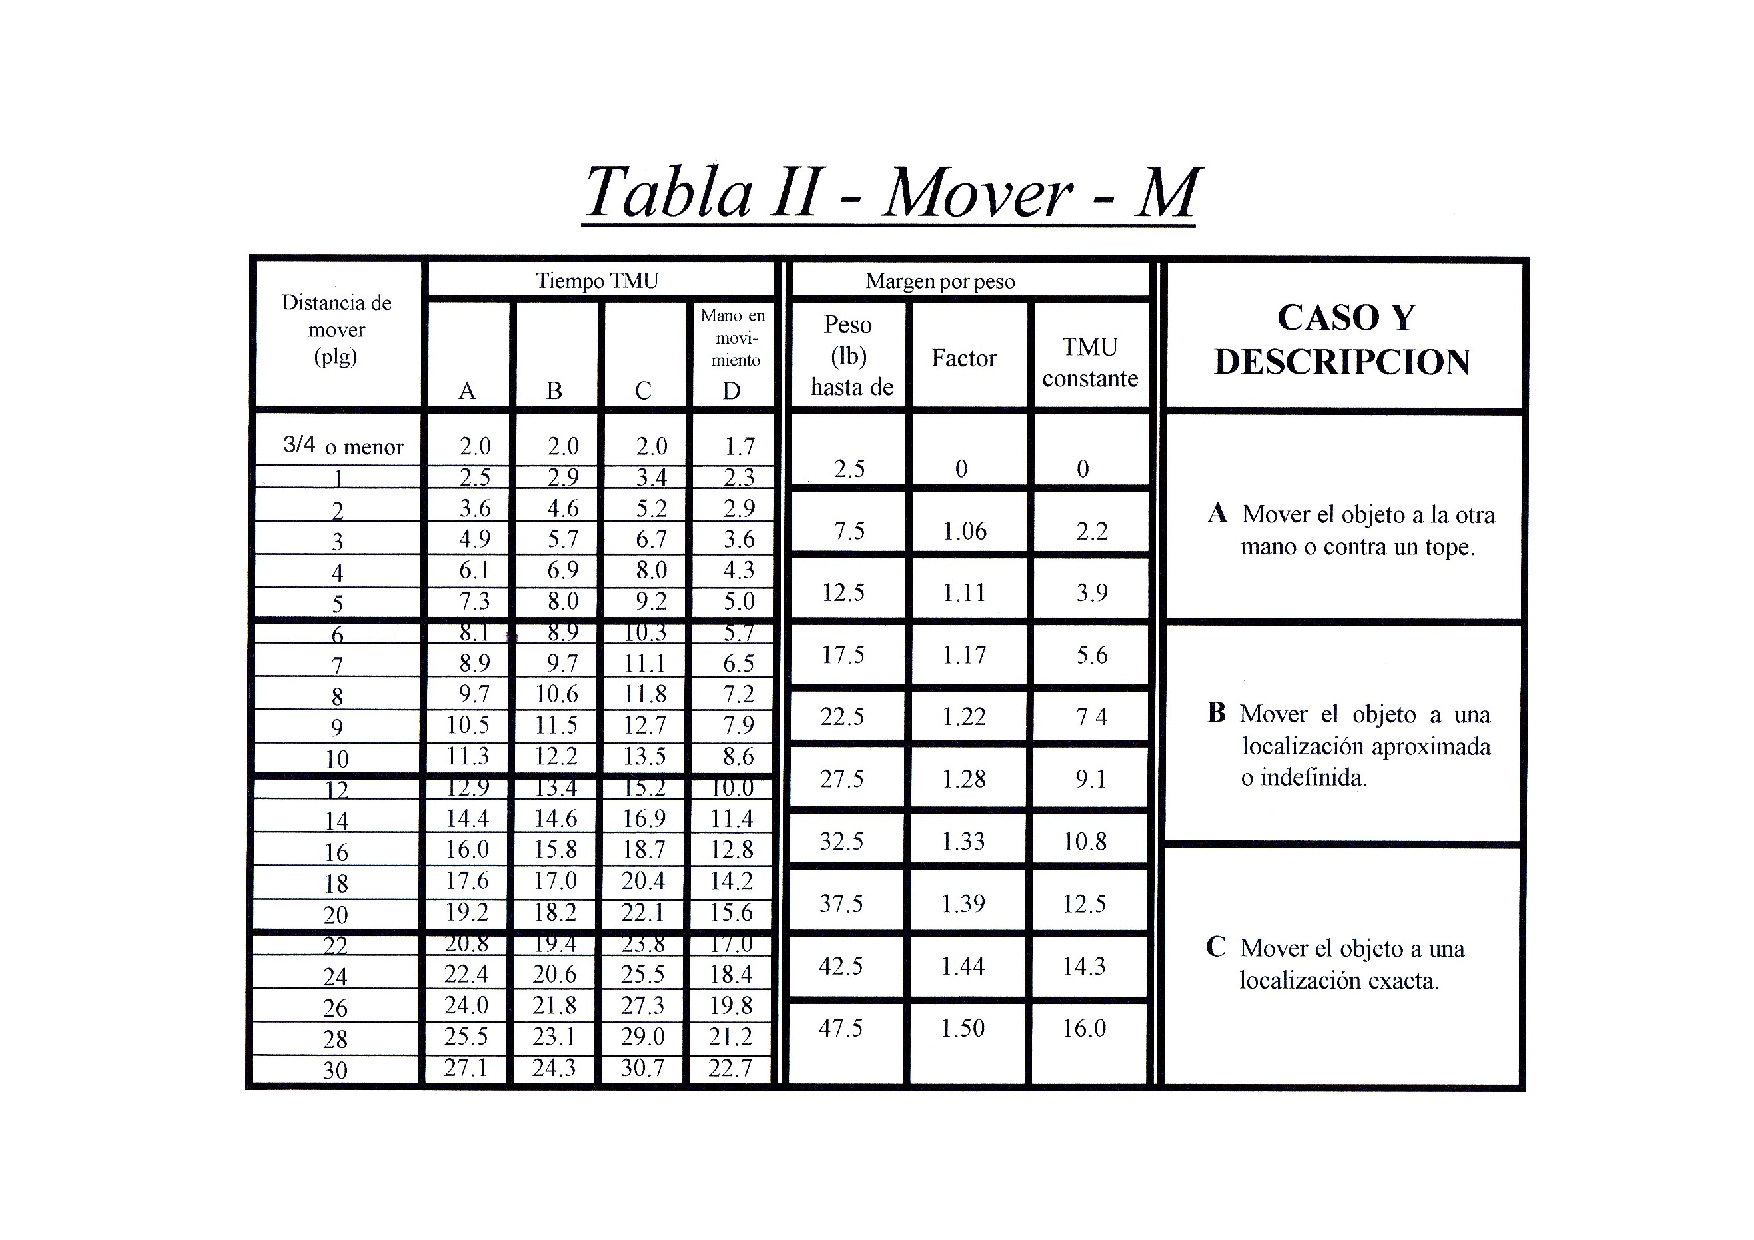
\includegraphics[trim = {0mm 0mm 0mm 15mm},clip,scale=0.3]{24/Img/tablaMover.pdf}
        \caption{TABLA- MOVER}
        \label{fig:Mover}
    \end{figure}
    %
    %
    \begin{figure}
        \centering
        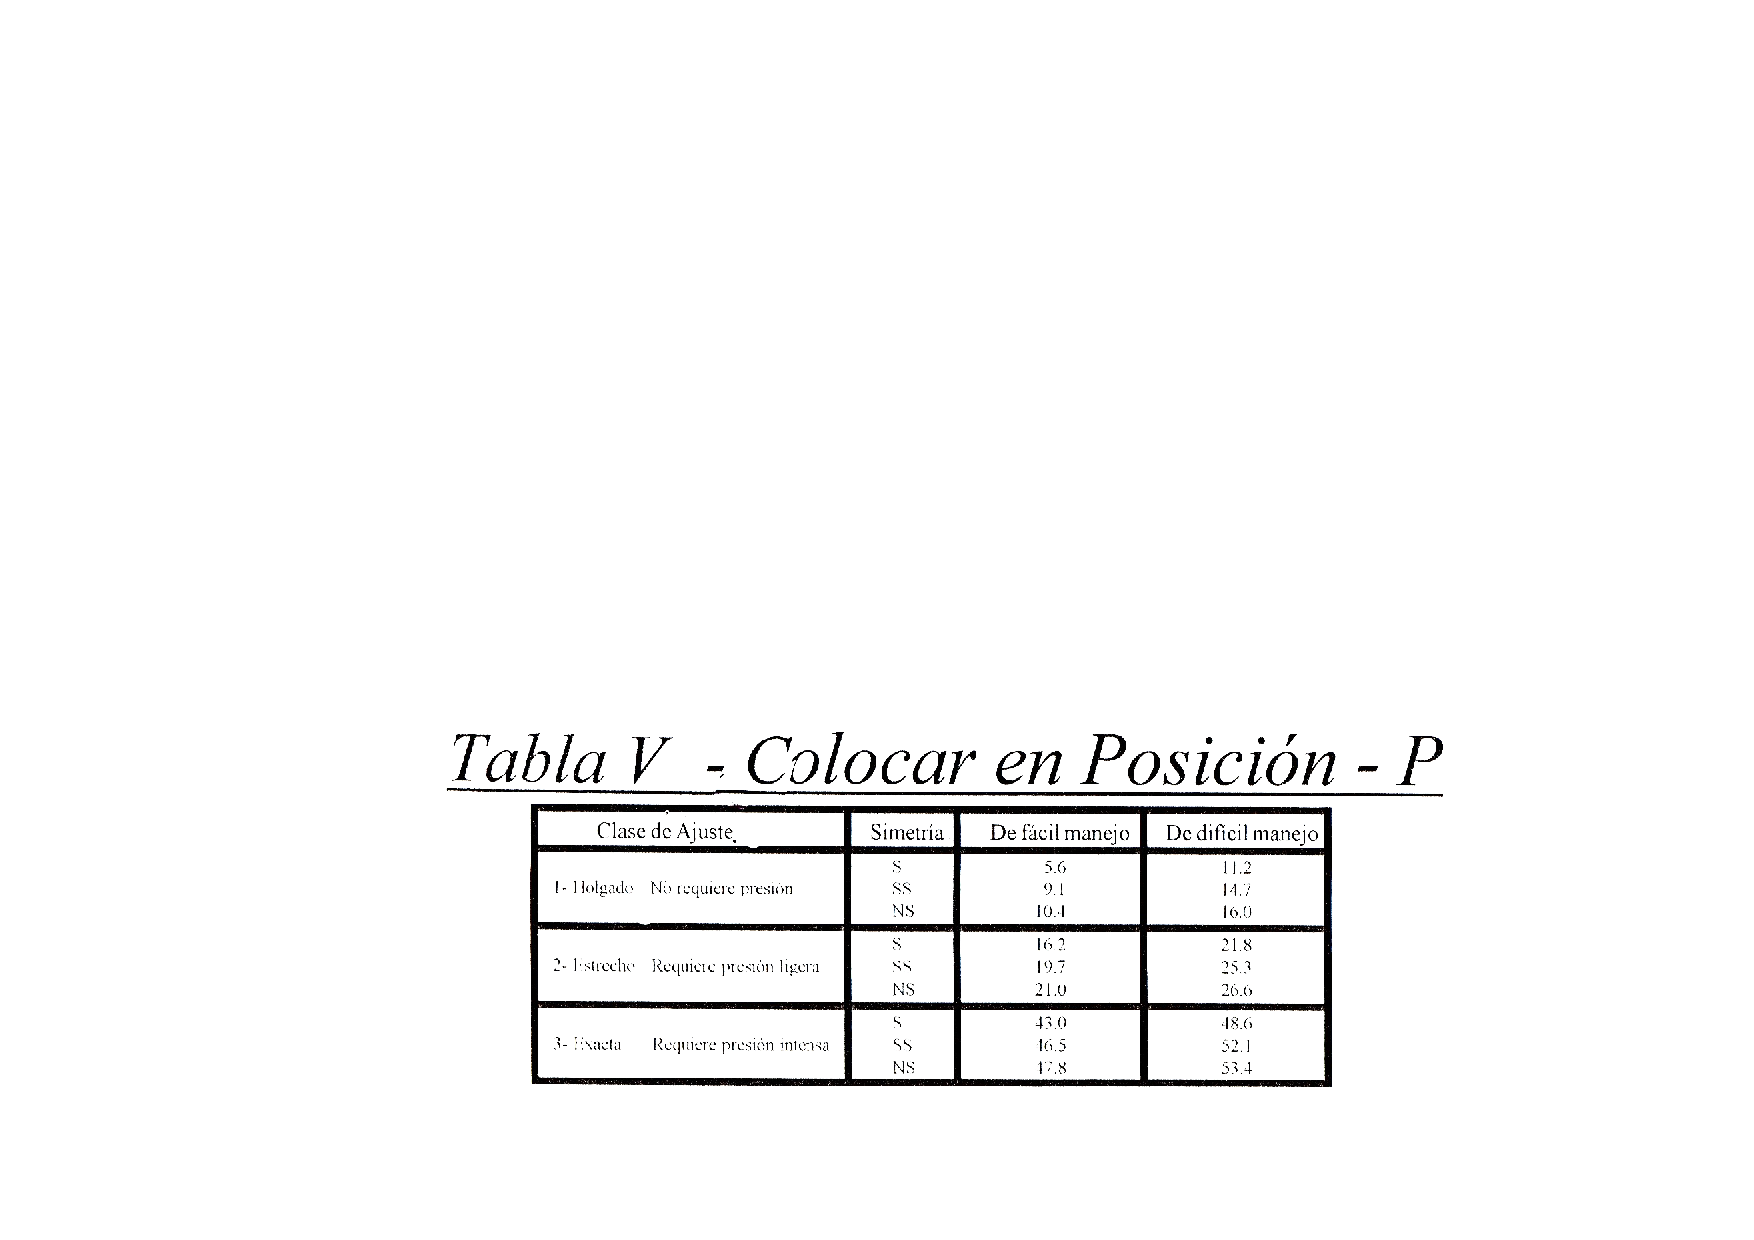
\includegraphics[trim = {0mm 0mm 0mm 13mm},clip,scale=0.3]{24/Img/tablaColocarPosicion.pdf}
        \caption{TABLA- COLOCAR POSICIONAR}
        \label{fig:COLOCAR}
    \end{figure}
    %
    %
    \begin{figure}
        \centering
        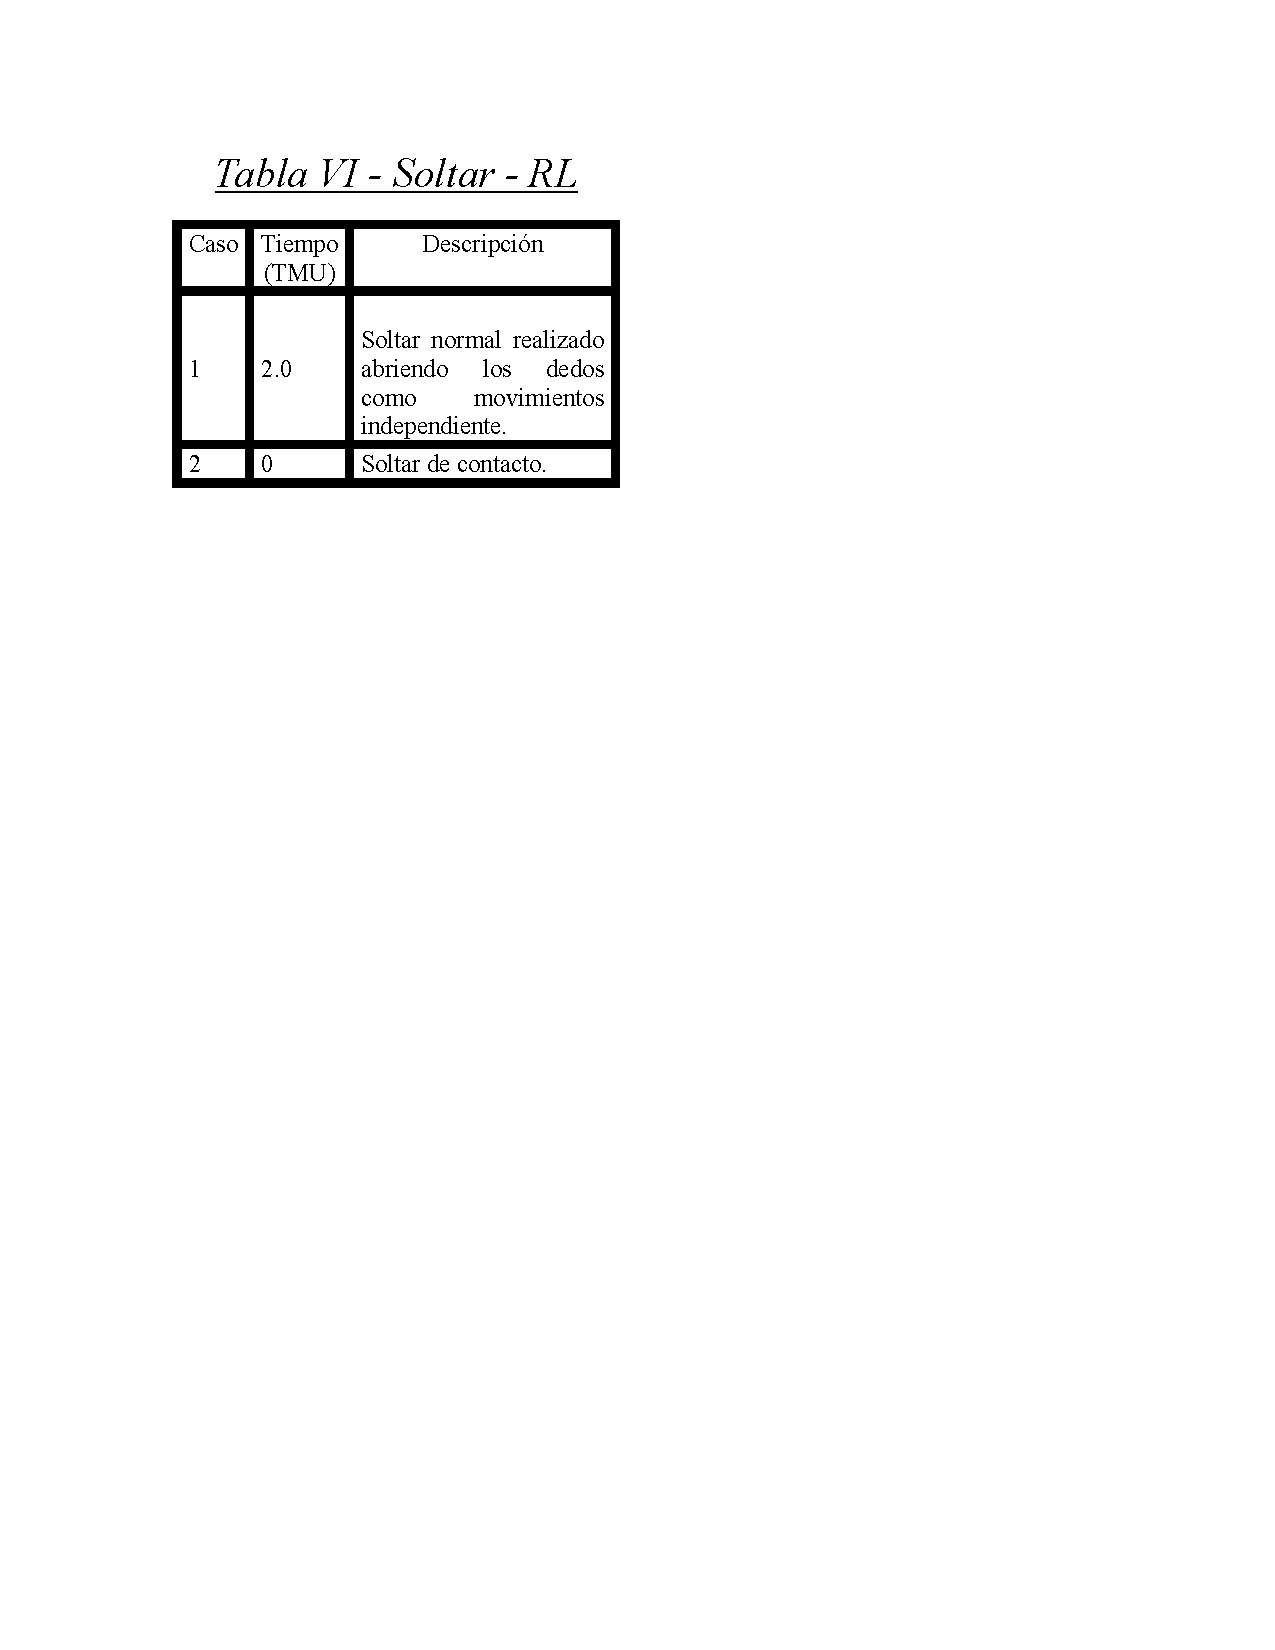
\includegraphics[trim = {0mm 0mm 0mm 13mm},clip,scale=0.3]{24/Img/tablaSoltar.pdf}
        \caption{TABLA- SOLTAR}
        \label{fig:SOLTAR}
    \end{figure}
    %
    %
    \subsubsection{Desarrollo del muestreo del trabajo}
    El propósito principal de este método es emplearlo como apoyo para lograr reducir los costos de operación. Para lograrlo tomamos 2 muestras de nuestro proceso de ensamblaje que nos ayudo a armar el circuito, estas muestras deben ser lo suficientemente buenas para representar el proceso completo, se analizaran los datos que recojamos de ellas. Usaremos estas muestras para calcular una estimación del tiempo de ciclo. Esto es importante porque, en lugar de medir el tiempo de cada ciclo del ensamblaje, solo necesitamos unas pocas mediciones representativas. Esto nos ahorra tiempo y recursos.
    %
    
    
    \subsubsection{Corrección por balanceo de procesos}
    La  utilización de la corrección por balanceo de procesos es una técnica esencial la cual se implementara en el proyecto integrador con el fin de distribuir las tareas de trabajo de manera más uniforme entre cada tarea para así mejorar muchos aspectos del proceso productivo.Como son, ayudar a evitar retrasos, mejorar el flujo de trabajo, usar mejor los recursos, mejorar la calidad del producto, ahorrar dinero, ser más flexibles y mejorar la satisfacción del personal. Todo esto hace que la producción sea más eficiente y competitiva, creando un entorno de trabajo más saludable y adaptable.
    %
    
    \subsubsection{Datos estándar continuos y discretos}
    %
    Trabajar con datos estándar implica seguir una serie de pasos para garantizar que los datos recopilados y utilizados sean representativos y precisos. Por eso es importante seleccionar las tareas a estudiar, recolectar datos, analizar datos, desarrollar datos estándar, implementar los datos estándar, monitorear y actualizar los datos estándar, posterior a esto tendremos que distinguir los elementos constantes y elementos variables.
    Tenemos como elemento constante aquel cuyo tiempo permanece igual ciclo tras ciclo, mientras que el elemento variable es aquel que varia dentro de un intervalo especifico de trabajo.
    
    %
    \subsection{Diseño de la forma más económica de realizar el trabajo}
    La primera etapa del estudio de trabajo nos ayuda a encontrar la forma más económica de hacer el trabajo es por ello que con el análisis de métodos, buscaremos comparar con otras técnicas, permitiéndonos hacer un estudio de análisis de reemplazo, el cuál permite a las empresas tomar decisiones informadas sobre la inversión en nuevos equipos, asegurando que los recursos se utilicen de manera óptima.Además de optimizar los costos, este estudio contribuye a mejorar la productividad y la calidad del trabajo. Evaluar y comparar diferentes métodos permite identificar ineficiencias y oportunidades de mejora ya que al reducir costos y mejorar la eficiencia, la empresa puede ofrecer productos de mejor calidad a precios más bajos, atrayendo a más clientes.
    
    \subsection{Normalización de los métodos, materiales, herramientas e instalaciones}
    La normalización de métodos, materiales, herramientas e instalaciones es vital para el éxito y la sostenibilidad de cualquier proyecto industrial. Al establecer y seguir estándares claros y uniformes, podemos asegurar la calidad, optimizar la eficiencia operativa, reducir costos, fomentar la innovación y mejorar la competitividad.
    La estandarización incluye la implementación de prácticas de seguridad reconocidas, lo que reduce significativamente el riesgo de accidentes y lesiones.Este enfoque no solo protege a los empleados, sino que también reduce los costos asociados con los accidentes laborales y las interrupciones en la producción, además que esta permite la optimización de procesos mediante la identificación y eliminación de ineficiencias. Esto resulta en una mayor productividad y en la reducción de los tiempos de ciclo.
    Adoptar estas prácticas no solo beneficia el proceso, sino que también mejora el bienestar de los operadores y la satisfacción de quienes consumen el producto, creando un círculo positivo de mejora continua y éxito empresarial.(Véanse los materiales en \ref{fig:lista-materiales})
    
    \subsection{Determinación del tiempo estándar para que una persona competente realice el trabajo con marcha normal}
    La determinación del tiempo estándar es un proceso detallado y sistemático que asegura la eficiencia y la precisión en la estimación del tiempo necesario para completar una tarea. Este proceso no solo ayuda a mejorar la planificación y la programación, sino que también contribuye a la mejora continua y la optimización de los recursos.
    \section{Resultados y discusión}
    
    \subsection{Desarrollo de la guía de plan de Emergencia}
    Para minimizar completamente las emergencias relacionadas con incendios y los riesgos de accidentes en el Instituto Tecnológico de Querétaro, hemos diseñado esta guía. Nuestro objetivo es identificar al personal que haya recibido capacitación al menos una vez al año, asegurando así que, en caso de emergencia, se tomen decisiones óptimas para proteger la integridad física tanto de los clientes internos como externos, así como de las instalaciones. Los detalles generales del establecimiento están resumidos en la Figura\ref{fig:mapa-itq}.
    % 
    % 
    \begin{figure}[H]
        \centering
        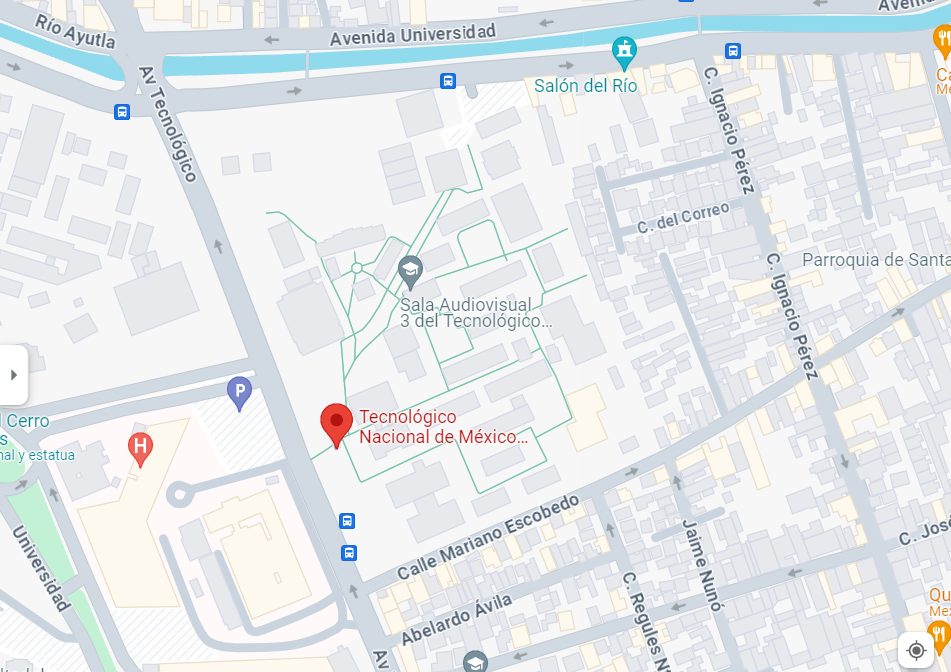
\includegraphics[scale=0.30]{24/Img/mapa-itq.png}
        \caption{Tecnológico Nacional de México, Instituto Tecnológico de Querétaro, Av Tecnológico S/N, Centro Histórico, Centro, 76000, Querétaro, Qro., 4422274400 Ext. 4423}
        \label{fig:mapa-itq}
    \end{figure}
    %
    \subsubsection{Identificación del riesgo}
    Nos comprometemos a mantener diariamente un programa de prevención de riesgos interno, además de recopilar retroalimentación de clientes internos y externos sobre los riesgos presentes en nuestras actividades diarias. Invitamos a todo el equipo de trabajo a participar activamente en este proceso. Cada riesgo interno se evaluará y clasificará según un rango de importancia para priorizar las acciones necesarias. A continuación, se puede consultar\ref{fig:RIESGOS} 
    %
    \begin{figure}
        \centering
        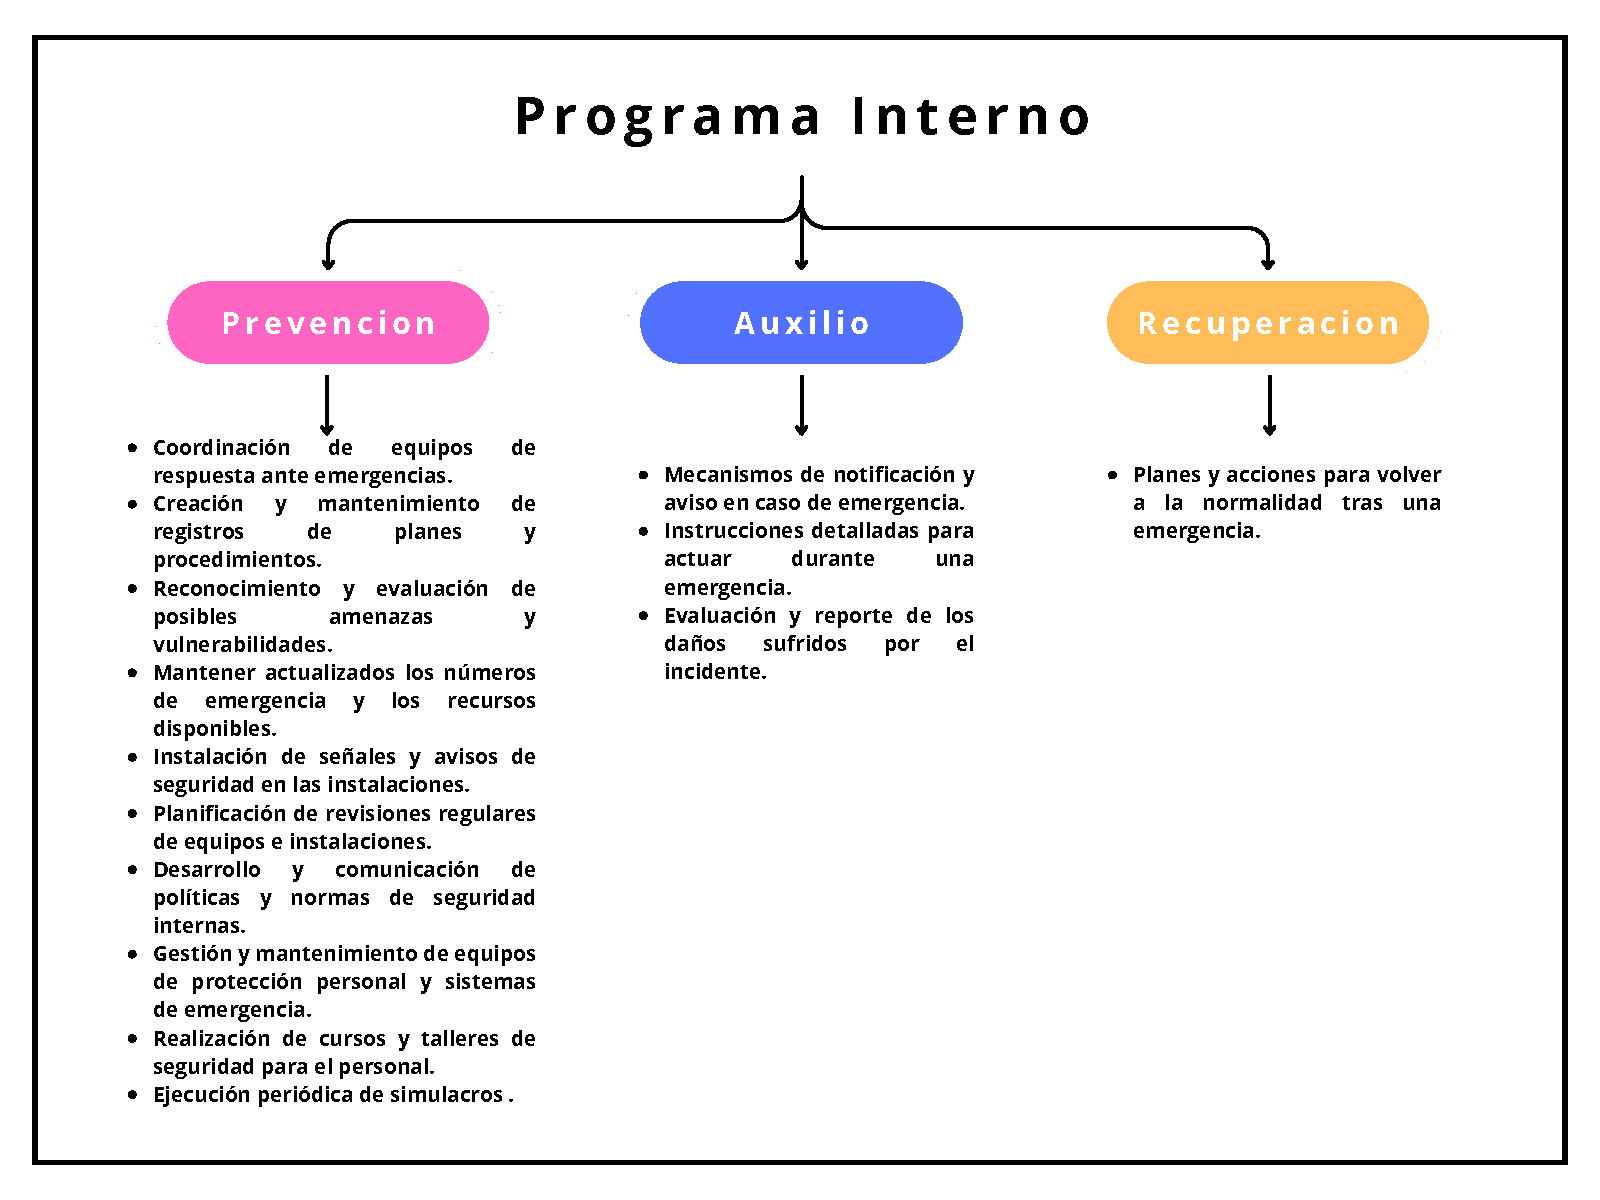
\includegraphics[trim = {0mm 0mm 0mm 0mm},clip,scale=0.3]{24/Img/programaInterno.pdf}
        \caption{IDENTIFICACIÓN DE RIESGOS}
        \label{fig:RIESGOS}
    \end{figure}
    %
    \subsubsection{Riesgos internos}
    Aquí mencionaremos las acciones de riesgo interno a las que la institución puede estar  expuesta. 
    Es por eso que el riesgo lo definimos como la probabilidad de que ocurra un evento adverso o perjudicial en algún aspecto dentro y fuera de la institución que afecte en su operación diaria, con estos aparatados podemos identificar la intensidad del riesgo así como las consecuencias que este podría traer.(La probabilidad de riesgos se puede ver en la siguiente imagen, \ref{Probabilidda de riesgos} y la descripción de los riesgos dentro de la empresa en\ref{Descripcion de riesgos})
    %
    \begin{figure}
        \centering
        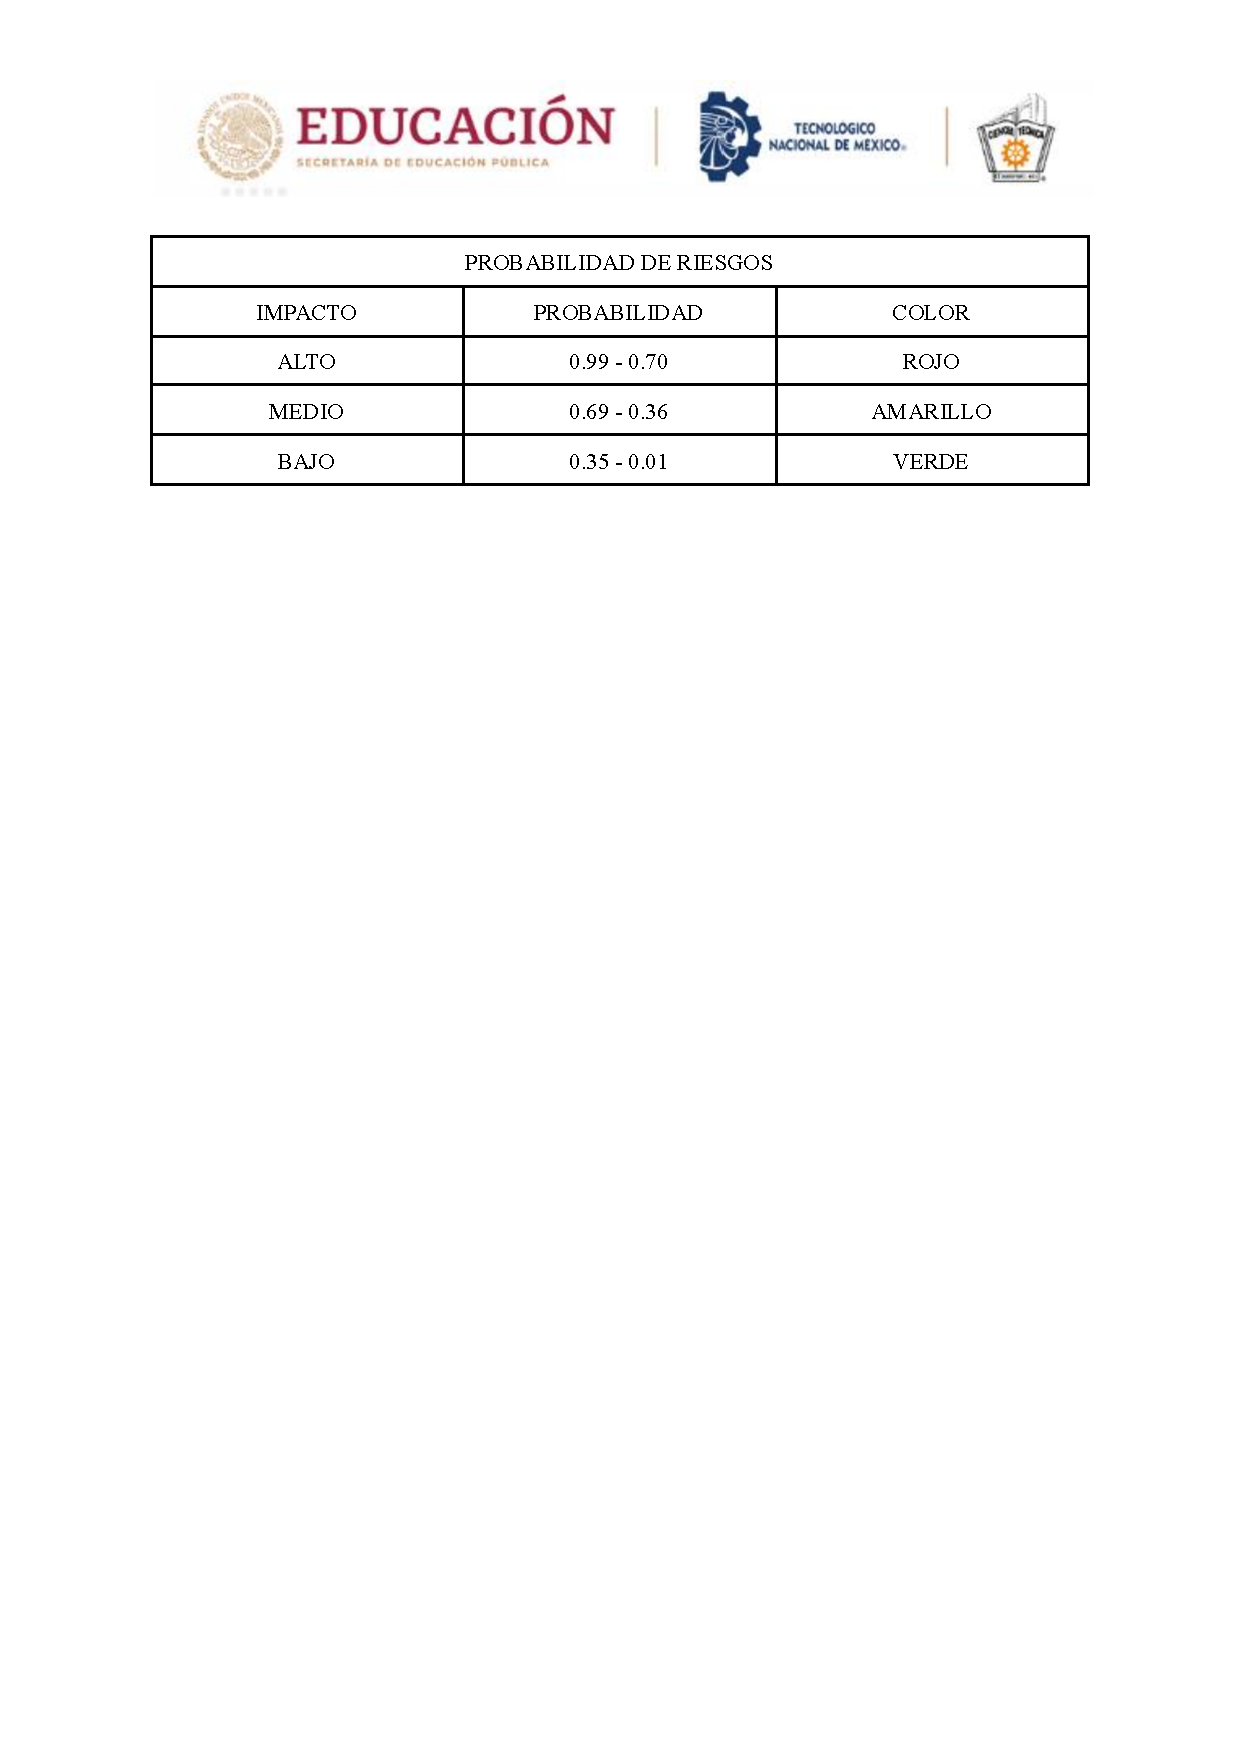
\includegraphics[trim = {0mm 210mm 0mm 0mm},clip,scale=0.3]{24/Img/probabilidaddeRiesgos.pdf}
        \caption{Riesgos con diferentes niveles y colores para distinguir la probabilidad}
        \label{Probabilidda de riesgos}
    \end{figure}
    %
    %
    \begin{figure}
        \centering
    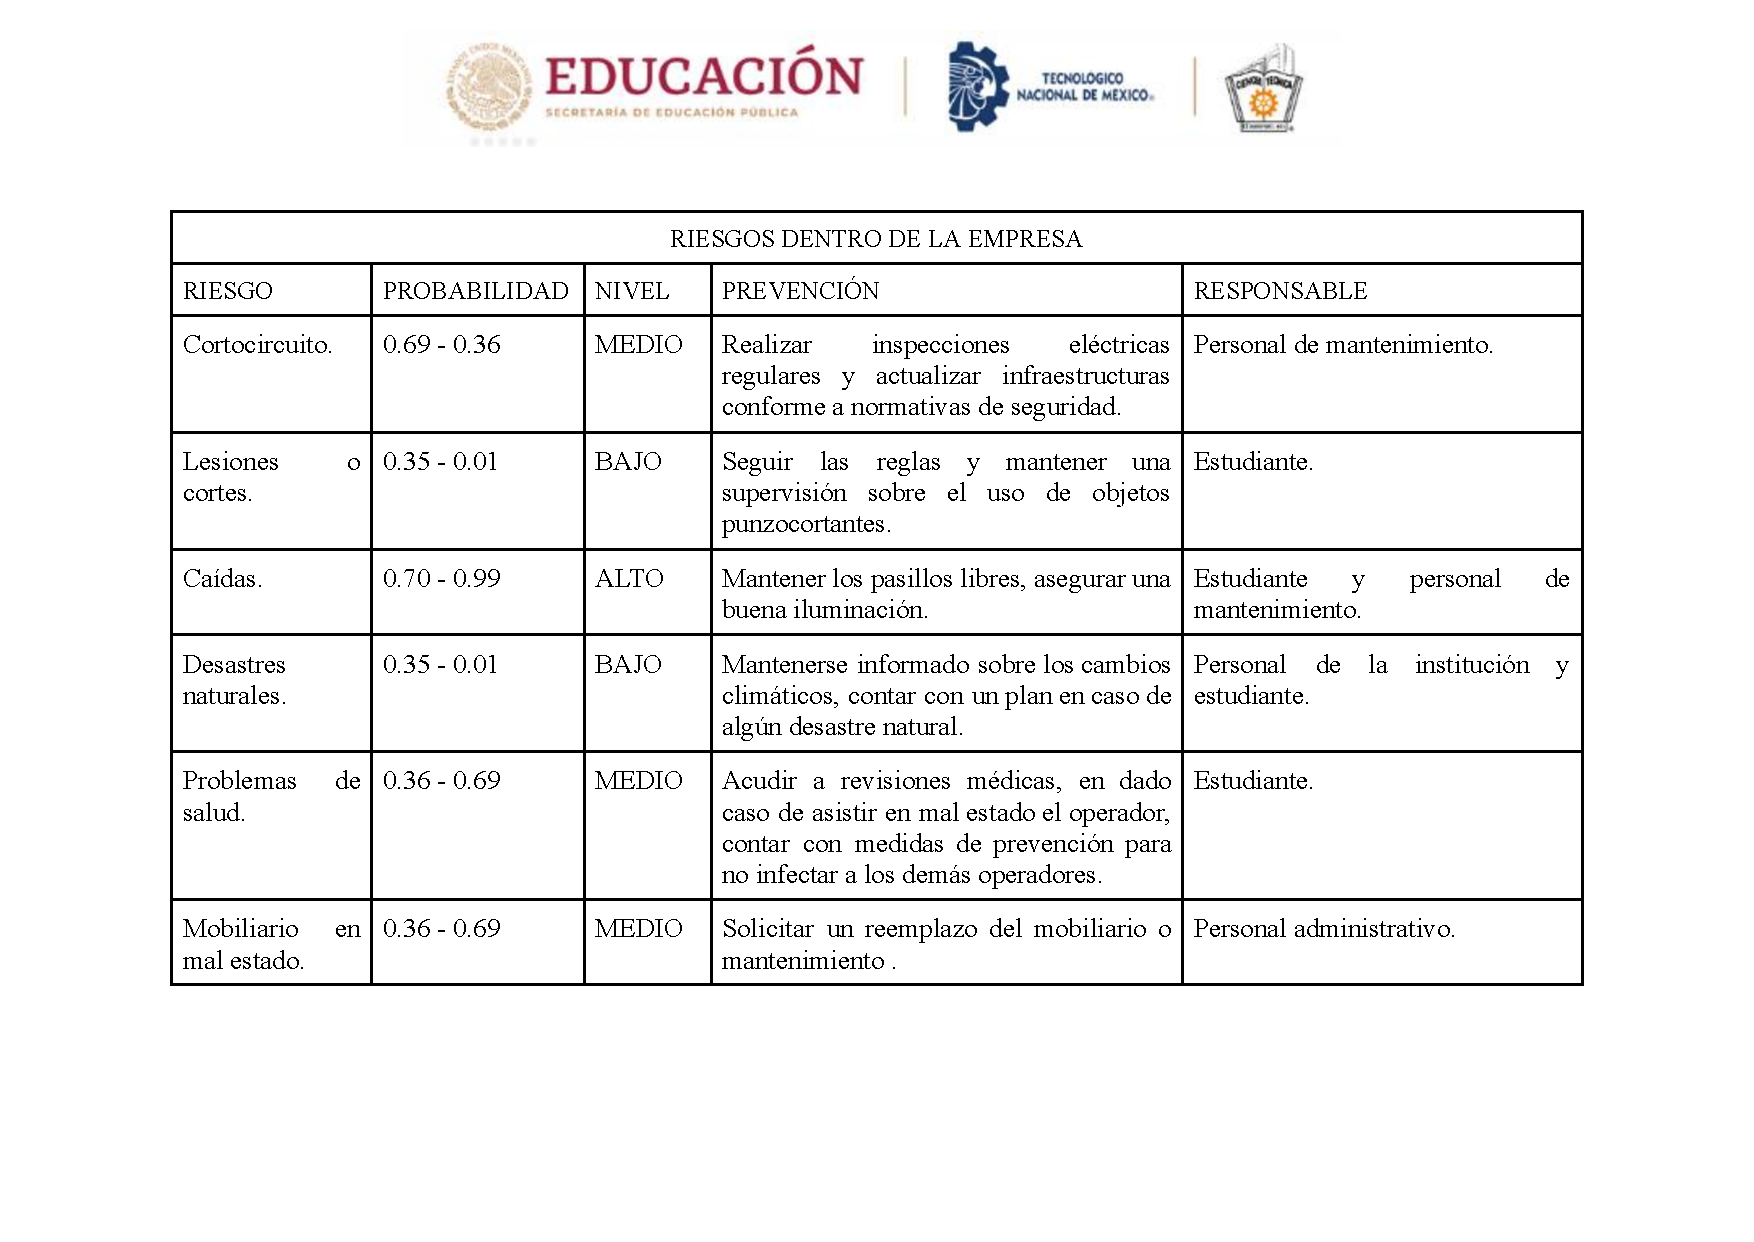
\includegraphics[trim = {0mm 30mm 0mm 0mm},clip,scale=0.3]{24/Img/descripciondeRiesgos.pdf}
        \caption{Descripción de los riesgos dentro de la Empresa.}
        \label{Descripcion de riesgos}
    \end{figure}
    %
    %
    \subsubsection{Riesgos externos}
    De la misma manera en que se identifican los riesgos internos, debemos tener presentes los externos, son aquellos que provienen del entorno fuera de la organización, esto incluye desastres naturales, incidentes ambientales o interrupciones en la cadena de suministros, generalmente son impredecibles y requieren planes de contingencia específicos para mitigar sus efectos. Véase en la figura \ref{Descripcion de riesgos externos} 
    %
    \begin{figure}
        \centering
    \includegraphics[trim = {0mm 30mm 0mm 0mm},clip,scale=0.3]{24/Img/descripciondeRiesgosExternos.pdf}
        \caption{Descripción de los riesgos externos a la Empresa.}
        \label{Descripcion de riesgos externos}
    \end{figure}
    %
    %
    \subsubsection{Programa de actividades de prevención y auxilio}
    Un Programa de Actividades de Prevención y Auxilio es un plan estructurado que se elabora para anticipar, evitar y responder eficazmente a situaciones de riesgo que puedan afectar a una organización o comunidad.Básicamente, estas son las medidas que se pretenden realizar antes de que ocurra un accidente.
    %
    %
    \subsubsection{Plan de acción}
    Un plan de acción es un conjunto estratégico de instrucciones que permite al Instituto Tecnológico de Querétaro (ITQ) realizar diversas tareas y funciones, enfocándose en la resolución de problemas y la gestión de riesgos tanto internos como externos. Este plan detalla los pasos a seguir para identificar, prevenir y mitigar posibles riesgos, así como las medidas de auxilio a tomar en caso de que ocurra un incidente. El objetivo de este es asegurar que todos dentro de la institución sepan que hacer para mantener la seguridad y la continuidad de las operaciones. Esto incluye la asignación de responsabilidades claras, la identificación de los recursos necesarios, la definición de plazos y la implementación de estrategias de seguimiento y evaluación continuas.\ref{Plan de accion} 
    %
    \begin{figure}
        \centering
    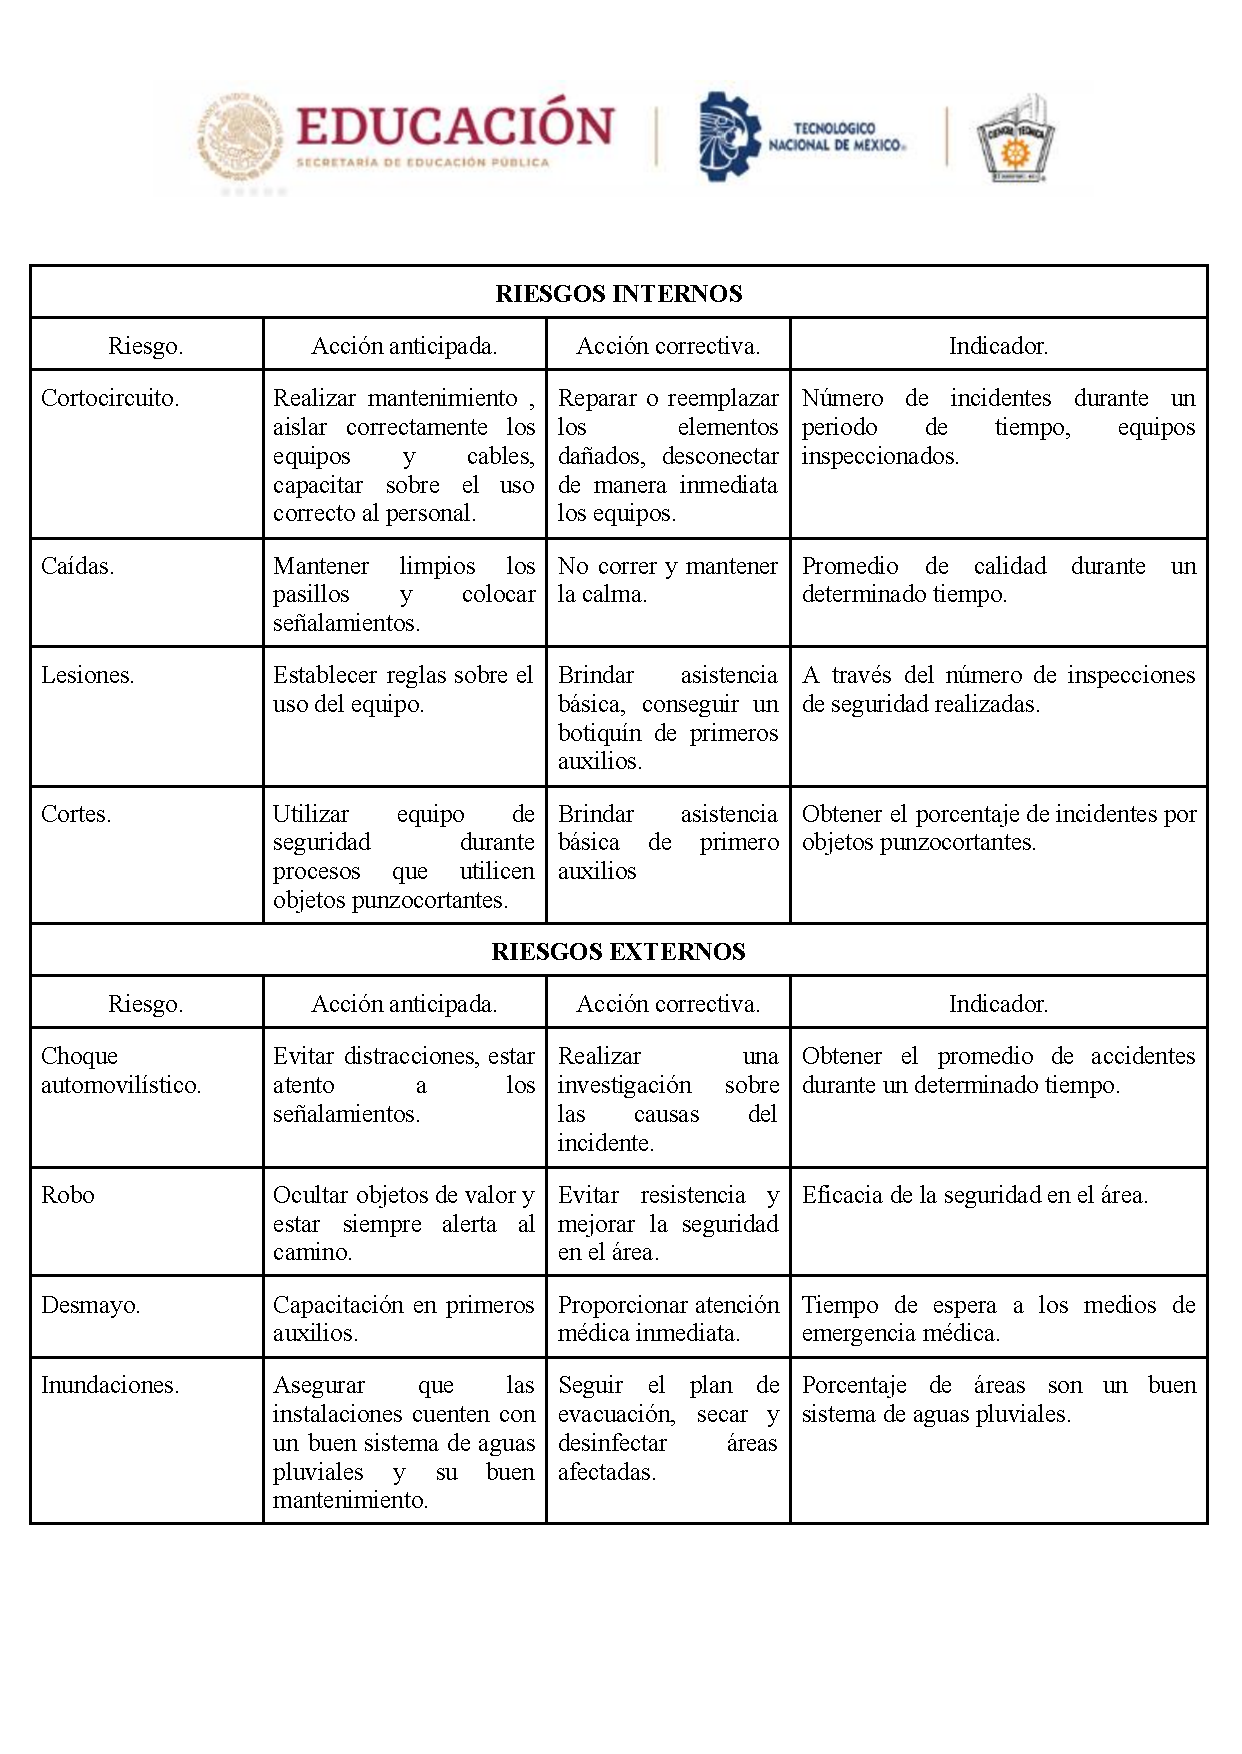
\includegraphics[trim = {0mm 30mm 0mm 0mm},clip,scale=0.3]{24/Img/plandeAccion.pdf}
        \caption{PLAN DE ACCION.}
        \label{Plan de accion}
    \end{figure}
    %
    %
    \subsubsection{Identificación de capacidades}
    En la tabla \ref{Material de seguridad.}, se puede encontrar el inventario de los materiales de seguridad dentro del Instituto Tecnológico de Queretaro. 
    %
    \begin{figure}
        \centering
    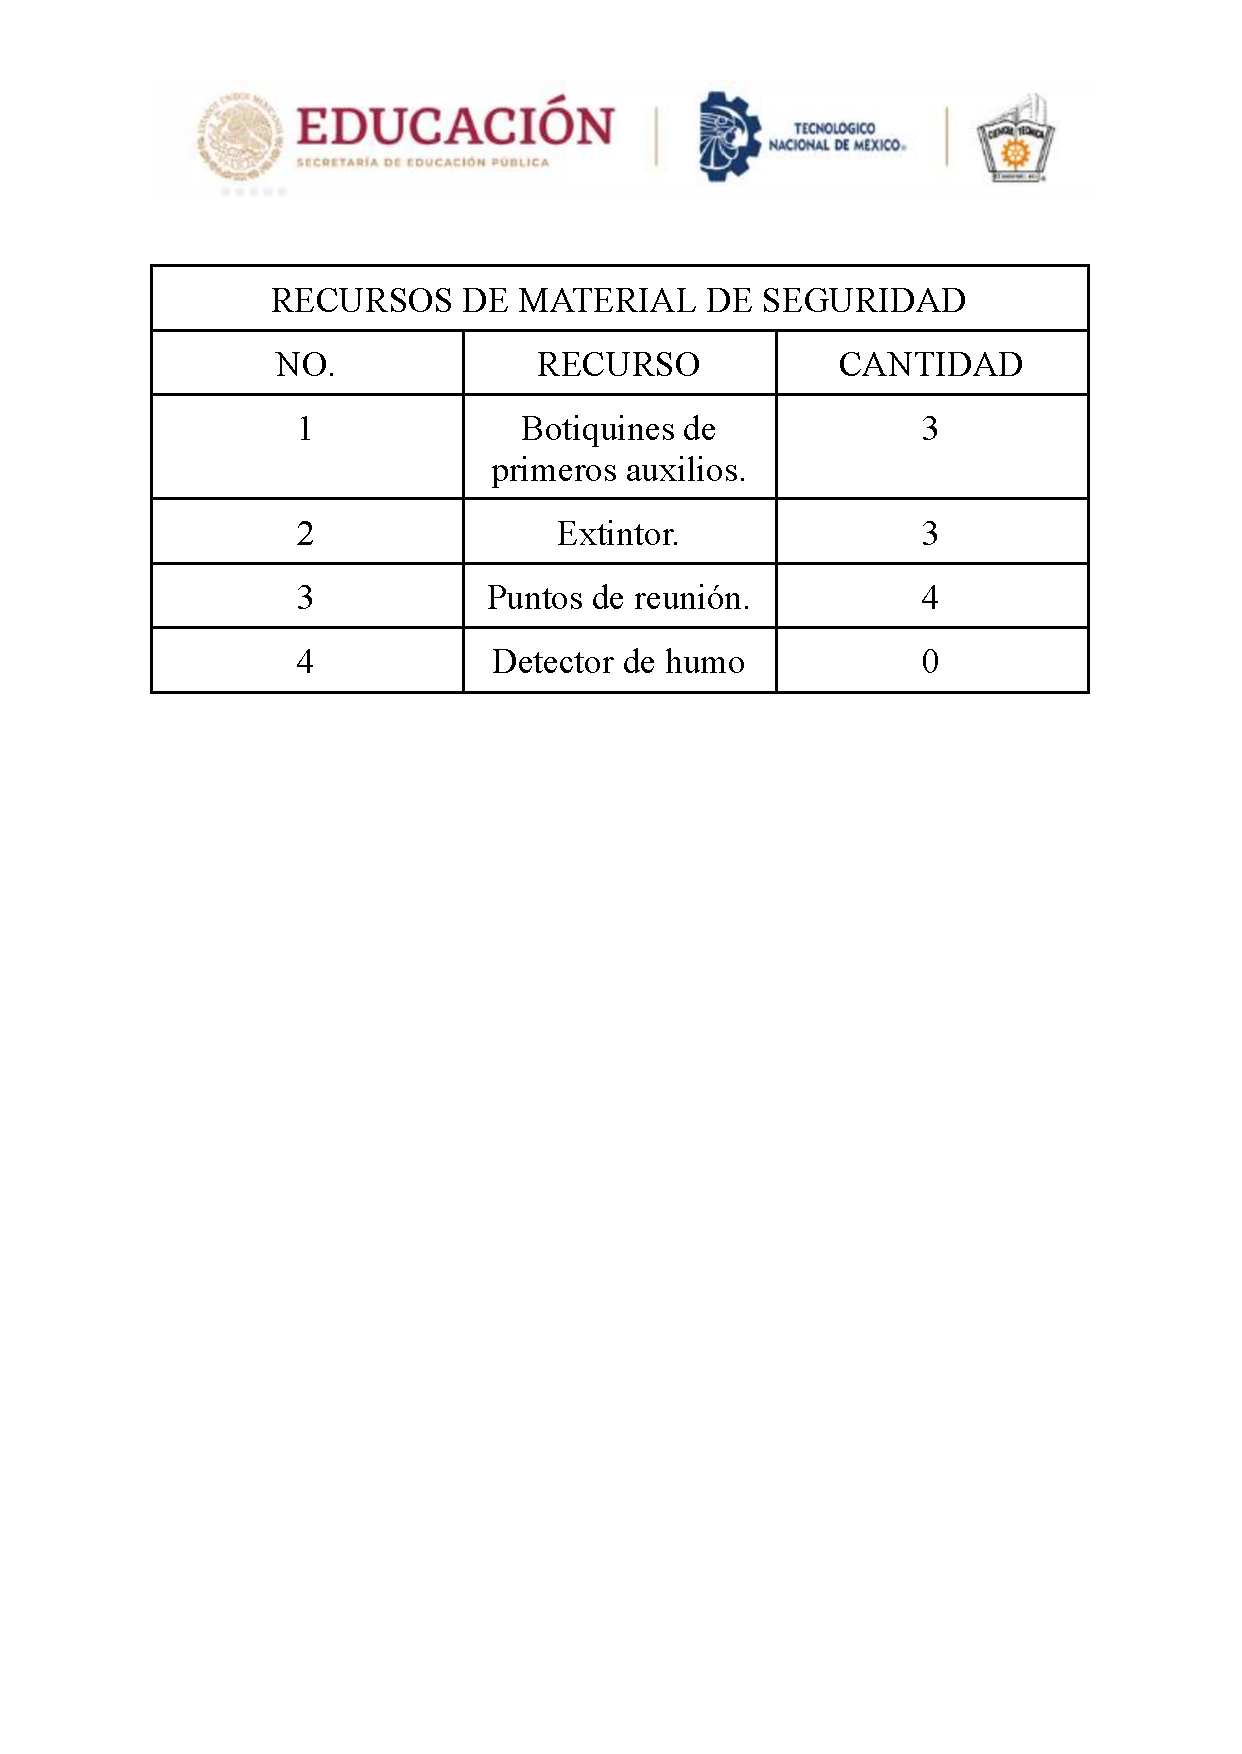
\includegraphics[trim = {0mm 150mm 0mm 0mm},clip,scale=0.3]{24/Img/materialdeSeguridad.pdf}
        \caption{MATERIALES DE SEGURIDAD}
        \label{Material de seguridad.}
    \end{figure}
    %
    %
    \subsubsection{Plano de localización de recursos}
    Para lograr una mejor visualización acerca de la distribución del material se a creado el plano de localización del material de seguridad, en el cual se ubica cada uno de los recursos mencionados en la tabla  \ref{Material de seguridad.}, Este croquis lo podremos en encontrar en la siguiente figura figura \ref{Localizacion del material}, 
    %
    \begin{figure}
        \centering
    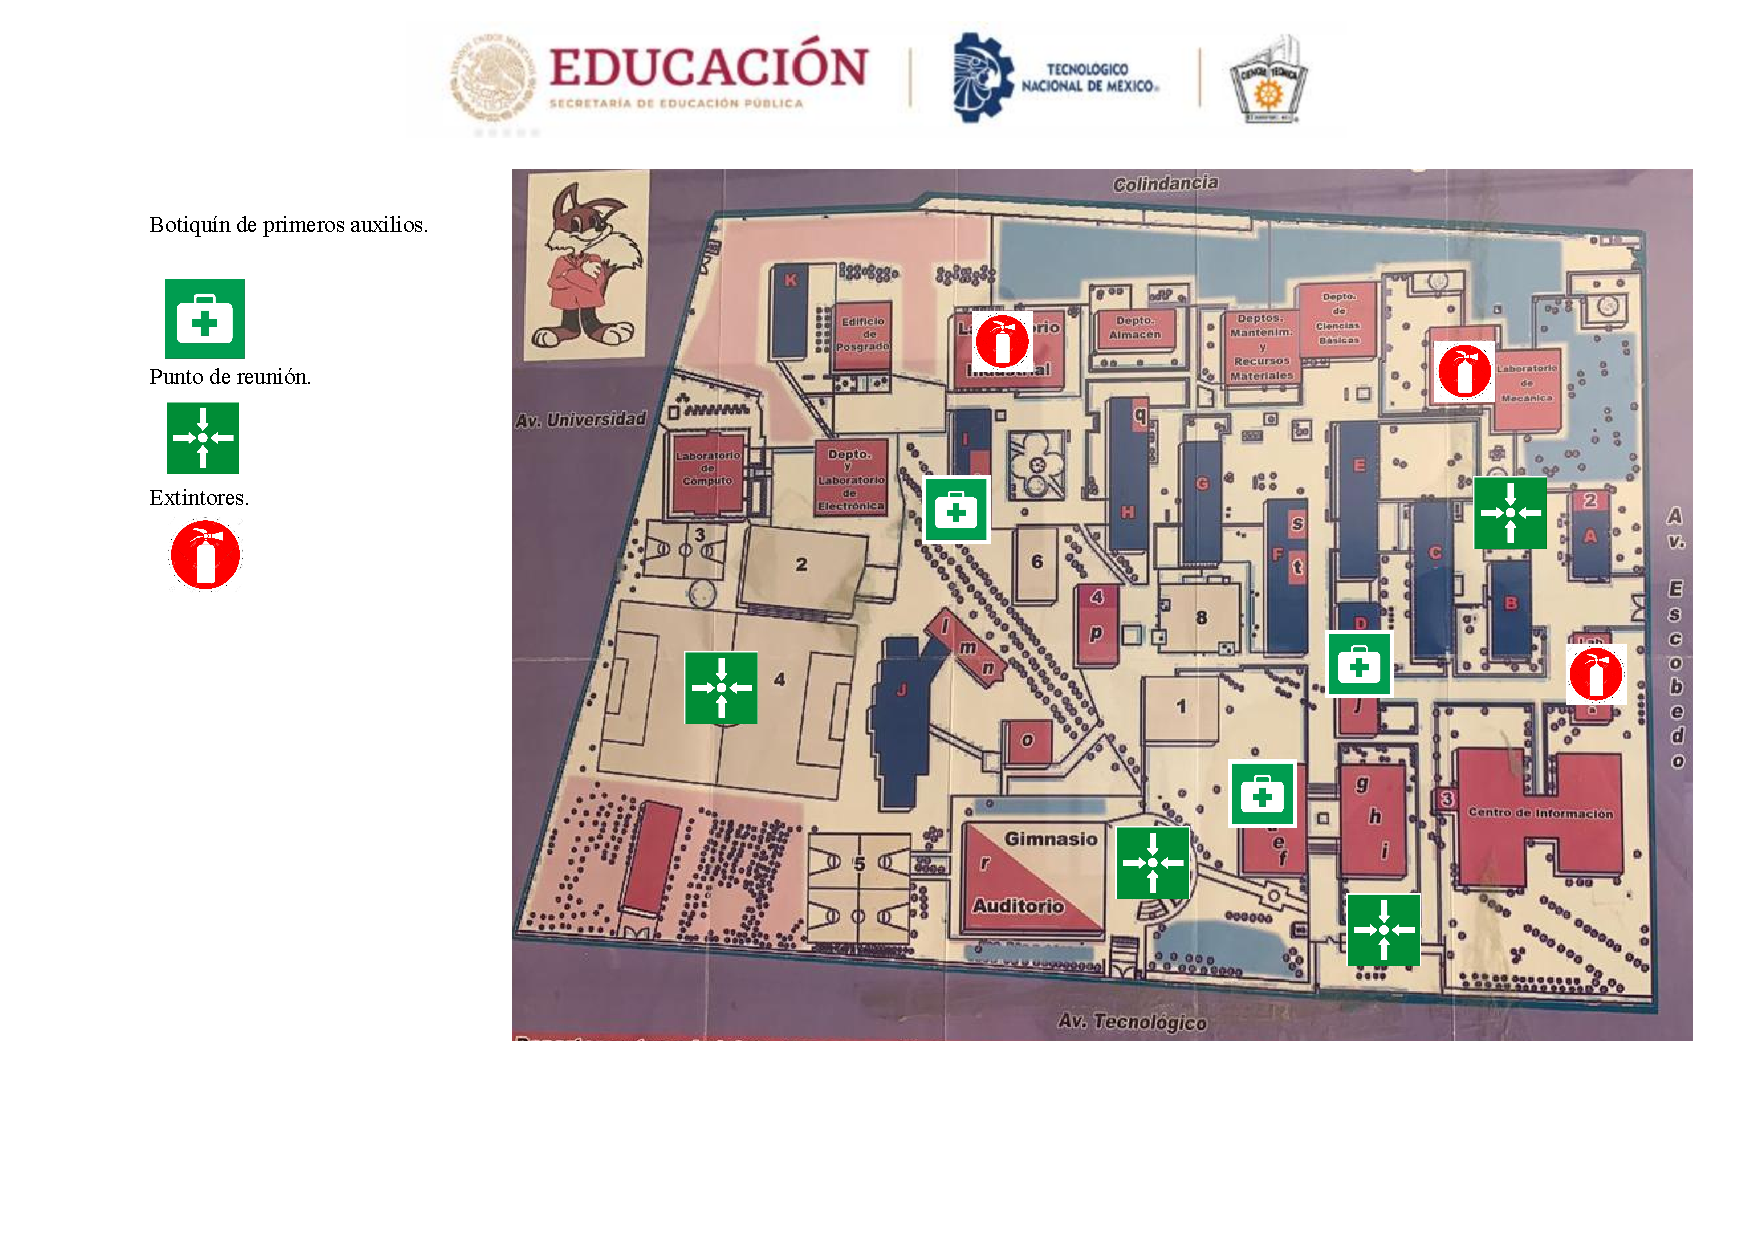
\includegraphics[trim = {0mm 0mm 0mm 0mm},clip,scale=0.3]{24/Img/planodeLocalizacion.pdf}
        \caption{PLANO DE LOCALIZACIÓN.}
        \label{Localizacion del material}
    \end{figure}
    %
    %
    \subsubsection{ Identificación de apoyos externos}
    El objetivo principal de este apartado es contar el poder contactar instituciones a las que podamos recurrir en caso de emergencia así como el numero telefónico y el tipo de servicio ofrecido, para que cualquier empleado pueda identificarlo de manera inmediata.\ref{Apoyos externos}
    %
    \begin{figure}
        \centering
    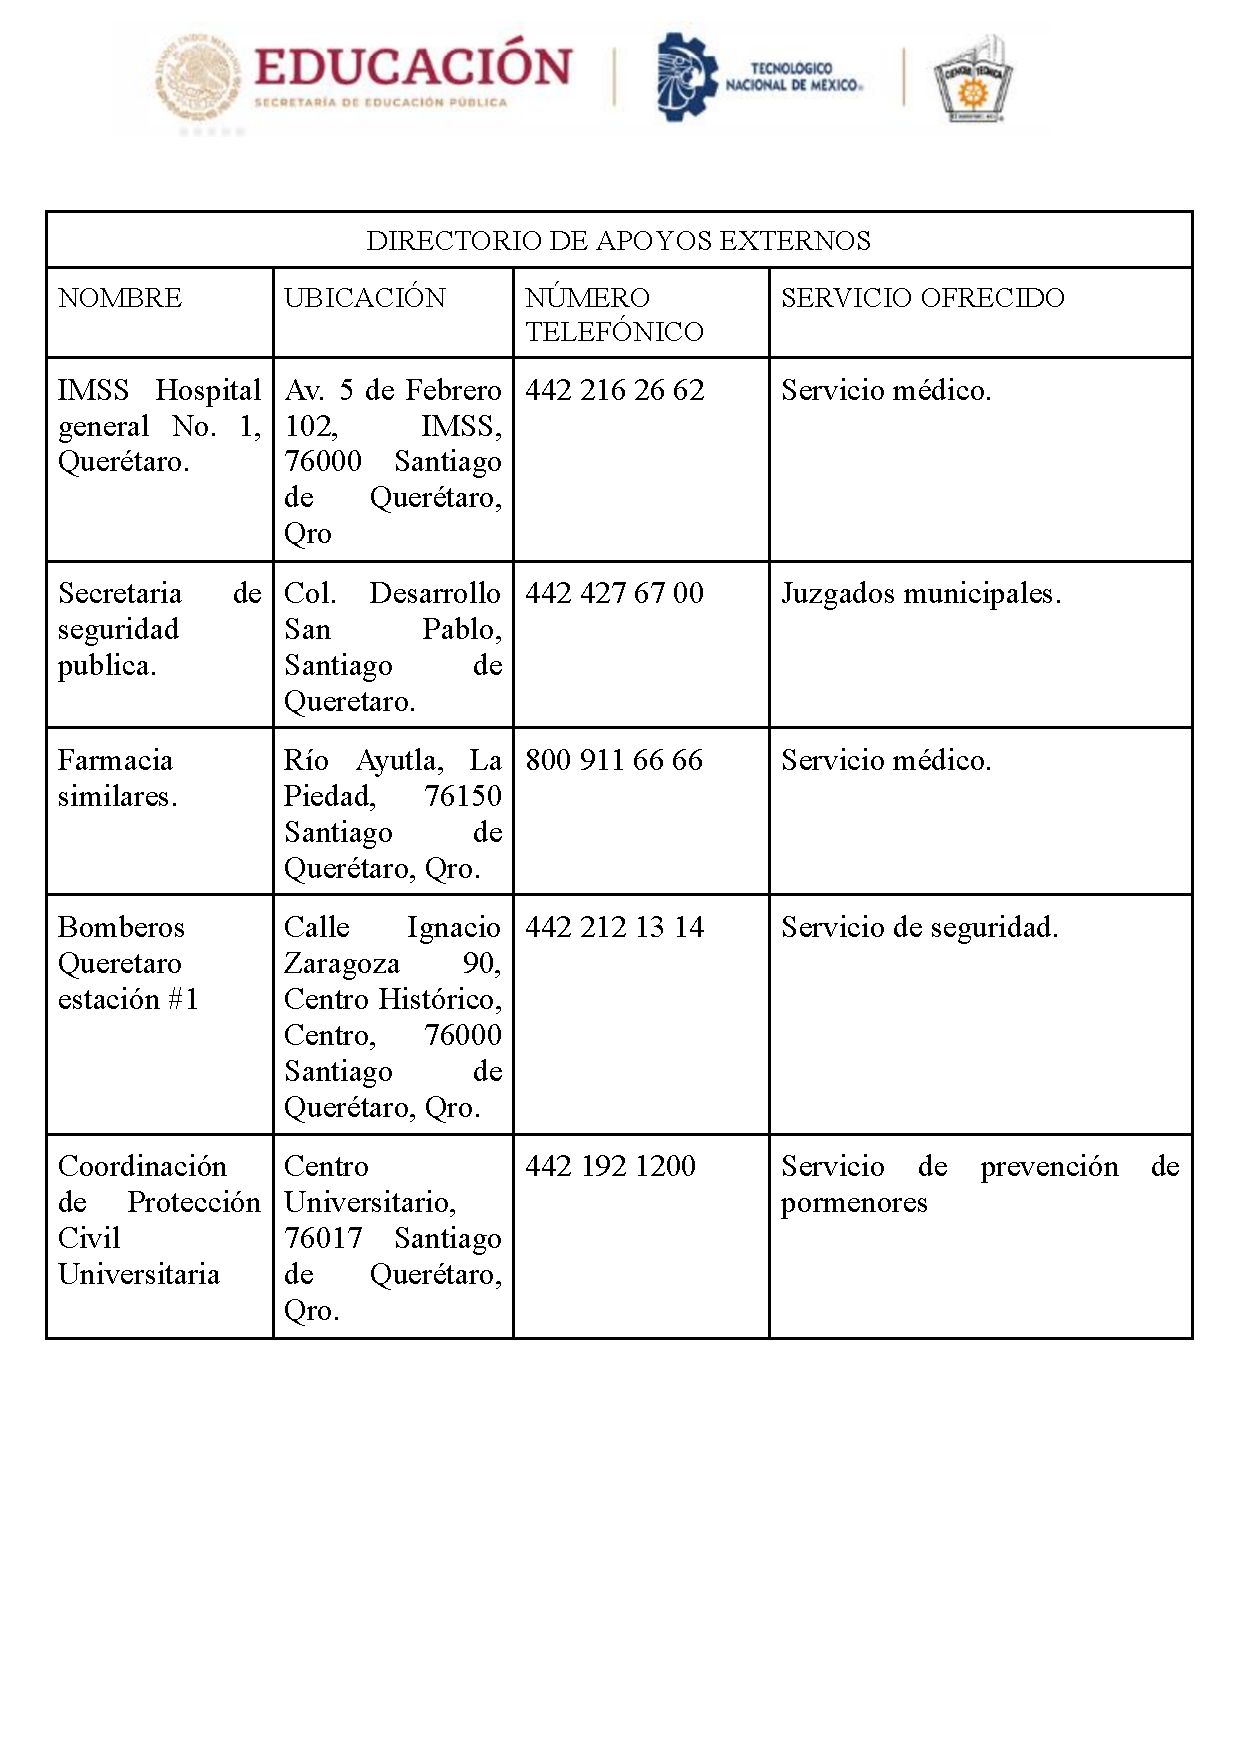
\includegraphics[trim = {0mm 50mm 0mm 0mm},clip,scale=0.3]{24/Img/directoriodeApoyosexternos.pdf}
        \caption{DIRECTORIO DE APOYOS EXTERNOS.}
        \label{Apoyos externos}
    \end{figure}
    %
    %
    \subsubsection{Identificación de puntos de reunión}
    La identificación de puntos de reunión implica determinar y señalizar ubicaciones específicas donde las personas deben congregarse en caso de una emergencia. Estos puntos se eligen por su seguridad y accesibilidad, y se señalan claramente para garantizar que todos los ocupantes del edificio puedan encontrarlos y llegar a ellos rápidamente. Este proceso es fundamental para asegurar una evacuación ordenada y eficiente, facilitando el conteo y la asistencia a todas las personas afectadas durante una situación de emergencia. Estos los podemos ubicar en la imagen \ref{Localizacion del material}. 
    %
    %
    \subsubsection{Brigada de evacuación}
    Una brigada de evacuación es un grupo de personas entrenadas dentro de una organización, cuya función es coordinar y dirigir la evacuación segura de todos los ocupantes durante una emergencia, como incendios o terremotos. Su objetivo principal es garantizar que la evacuación se realice de manera ordenada y eficiente, proporcionando asistencia y asegurando que todos sigan las rutas de escape designadas. A continuación se muestran los roles de nuestra brigada de evacuación \ref{BRIGADA DE EVACUACION}
    %
    \begin{figure}
        \centering
    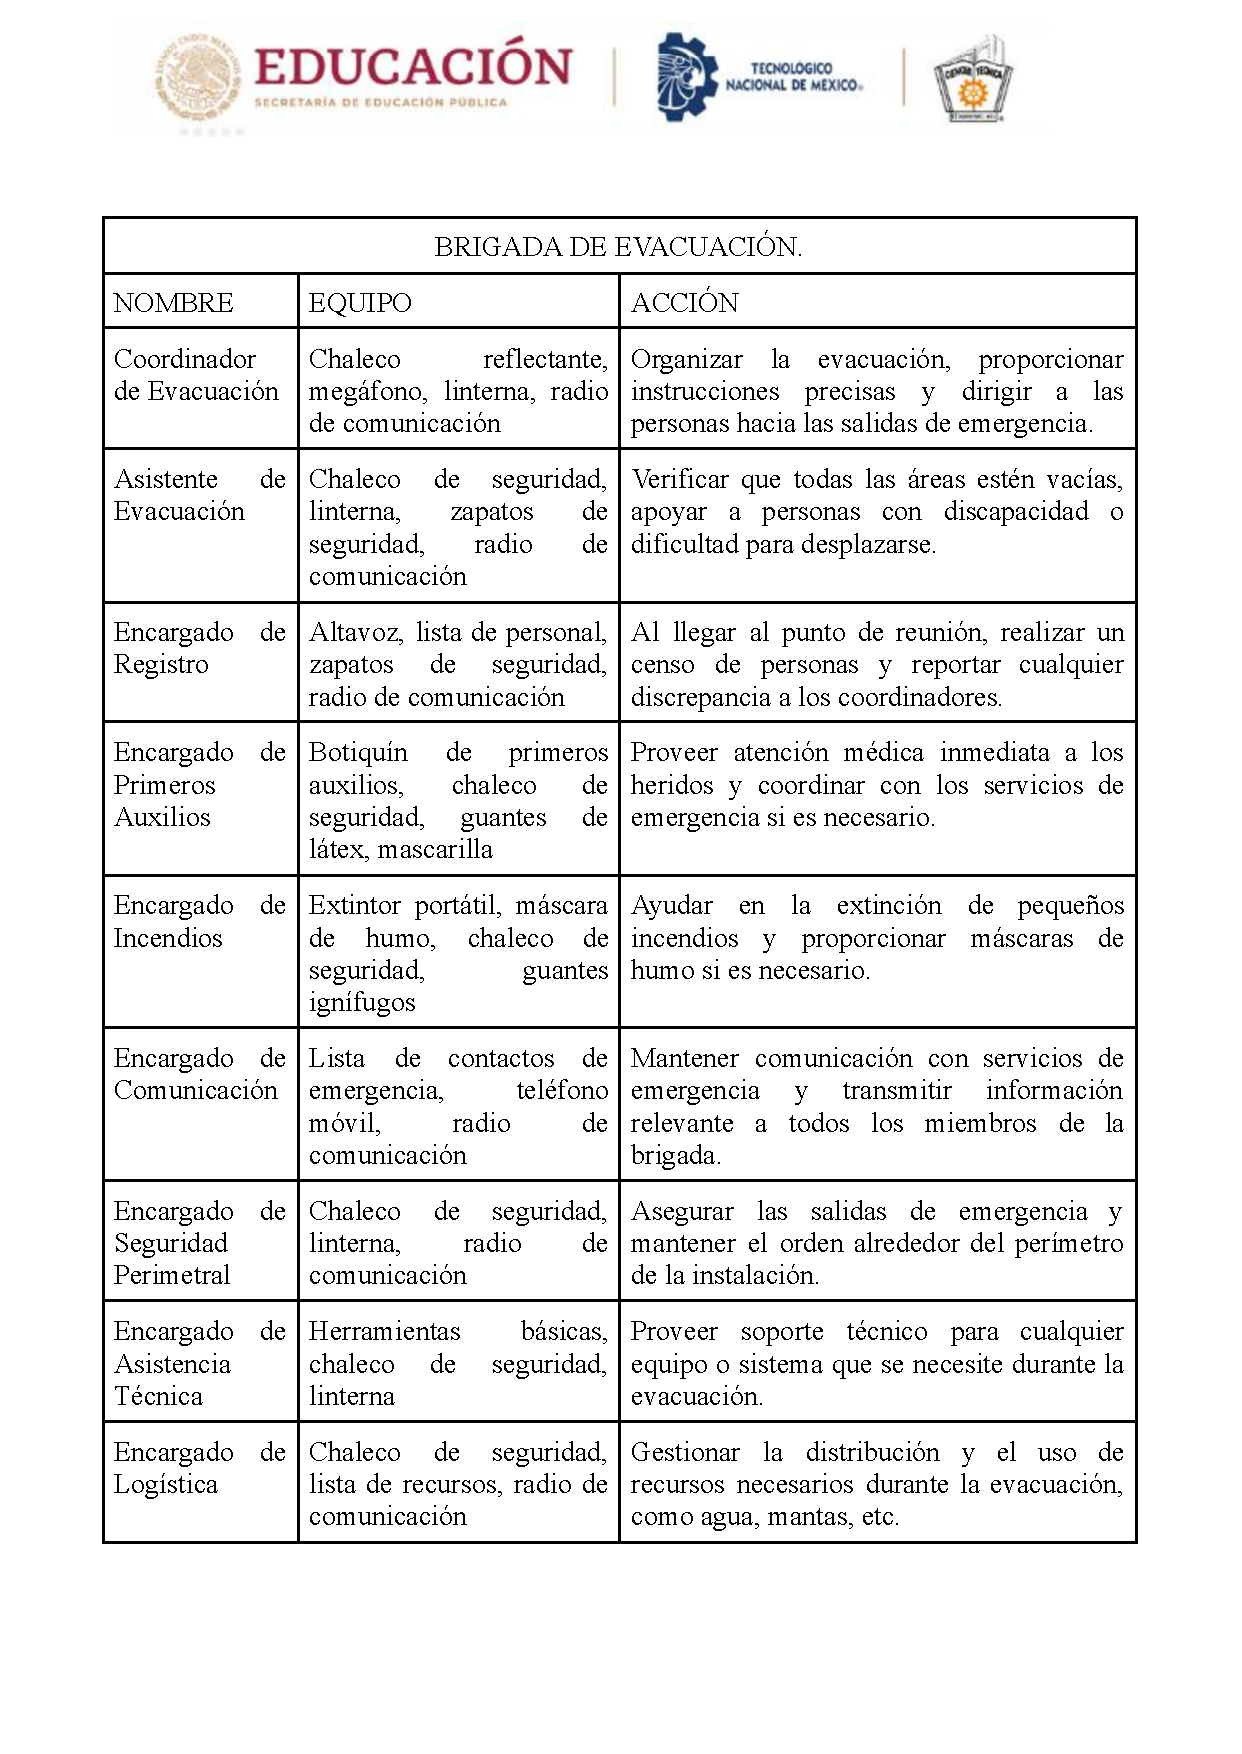
\includegraphics[trim = {0mm 0mm 0mm 0mm},clip,scale=0.3]{24/Img/brigadadeEvacuacion.pdf}
        \caption{BRIGADA DE EVACUACIÓN.}
        \label{BRIGADA DE EVACUACION}
    \end{figure}
    %
    %
    \subsubsection{Directorio de telefónicos de emergencia}
    Un directorio telefónico de emergencias es una lista de números de contactos cruciales que se utilizan en situaciones de emergencia, incluye números de servicios como bomberos, policía, ambulancias, hospitales y personal de seguridad interna, facilitando una respuesta rápida y eficiente ante incidentes críticos. Los cuales se pueden consultar en la imagen\ref{DIRECTORIO TELEFONICO}.
    %
    \begin{figure}
        \centering
    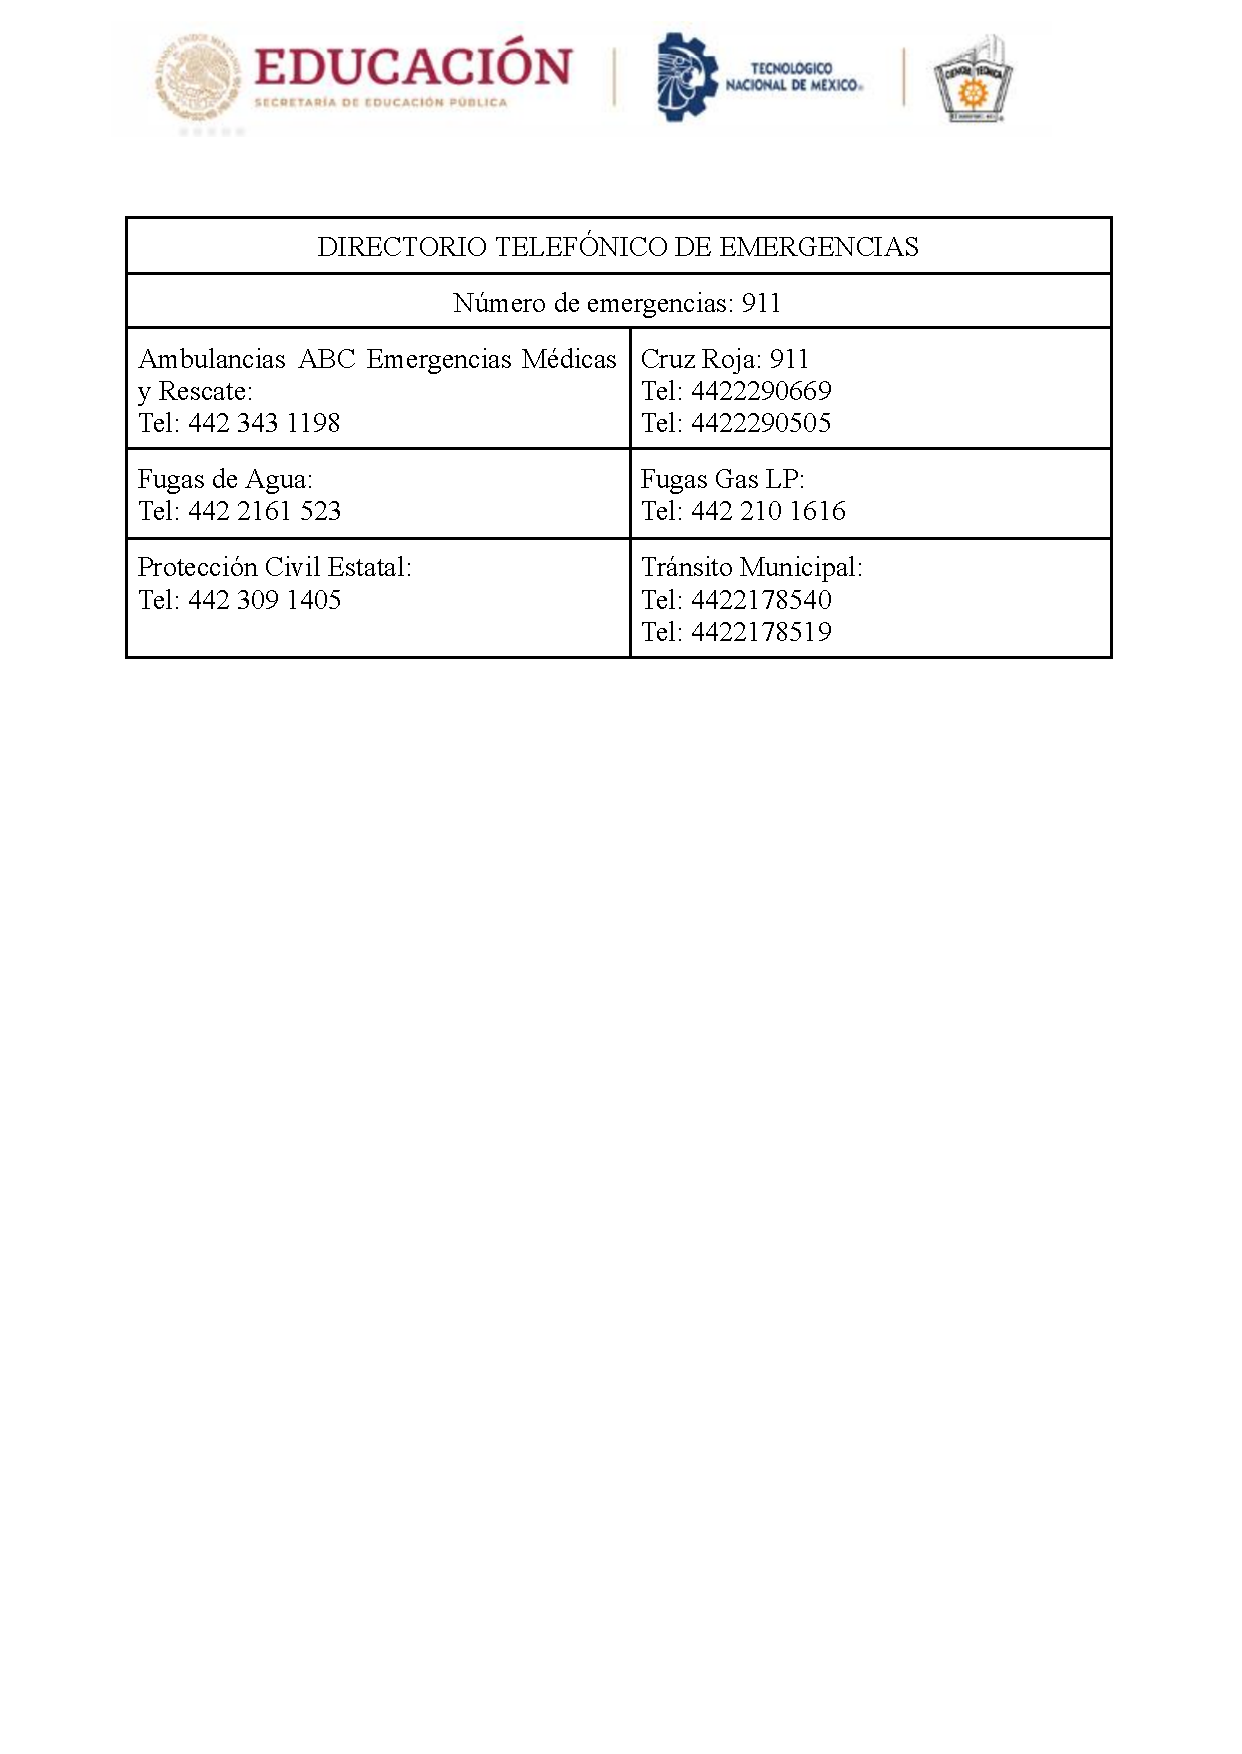
\includegraphics[trim = {0mm 180mm 0mm 0mm},clip,scale=0.3]{24/Img/directorioTelefonico.pdf}
    \caption{DIRECTORIO TELEFÓNICO DE EMERGENCIAS}
        \label{DIRECTORIO TELEFONICO}
    \end{figure}
    %
    %
    \subsection{Análisis de los métodos, materiales, herramientas e instalación utilizada en la ejecución del ensamble de un circuito electrónico}
    El análisis de los métodos, materiales, herramientas e instalación utilizados en la ejecución del ensamble de un circuito electrónico consiste en evaluar y optimizar los procedimientos y recursos empleados para ensamblar componentes electrónicos. Este análisis incluye la selección adecuada de materiales y herramientas, así como la configuración de la instalación para garantizar eficiencia, calidad y seguridad en el proceso de ensamblaje. Por eso a continuación se muestra una tabla Bianual del proceso de ensamblaje de nuestro circuito eléctrico.(\ref{fig:Diagrama Bimanual}, \ref{fig:Diagrama Bimanual2}, \ref{fig:Diagrama Bimanual3}, \ref{fig:Diagrama Bimanual4}) 
    %
    \begin{figure}
        \centering
        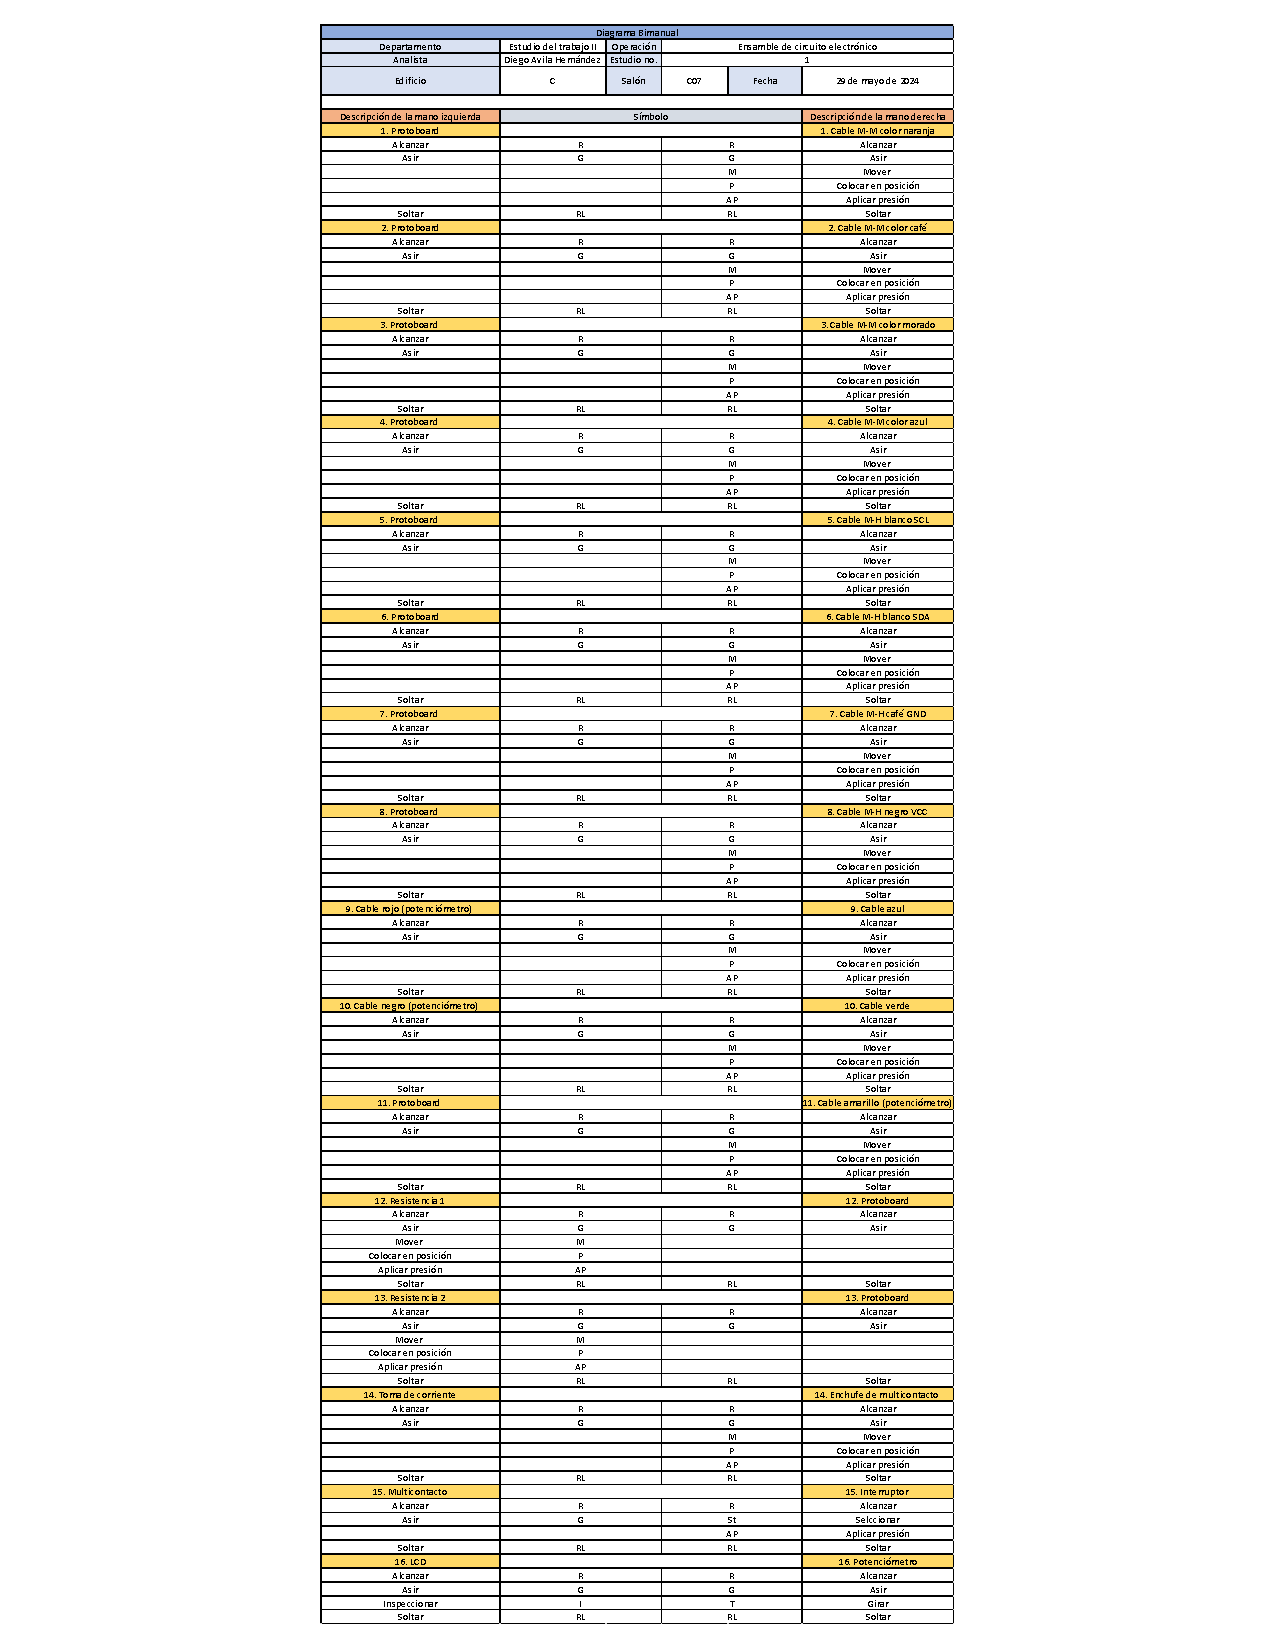
\includegraphics[trim = {5mm 5mm 5mm 10mm},clip,scale=0.30]{24/Img/diagramaBimanual1.pdf}
        \caption{Diagrama Bimanual}
        \label{fig:Diagrama Bimanual}
    \end{figure}
    %
    \begin{figure}
        \centering
        \includegraphics[trim = {5mm 15mm 5mm 10mm},clip,scale=0.3]{24/Img/diagramaBimanual2.pdf}
        \caption{}
        \label{fig:Diagrama Bimanual2}
    \end{figure}
    %
    \begin{figure}
        \centering
        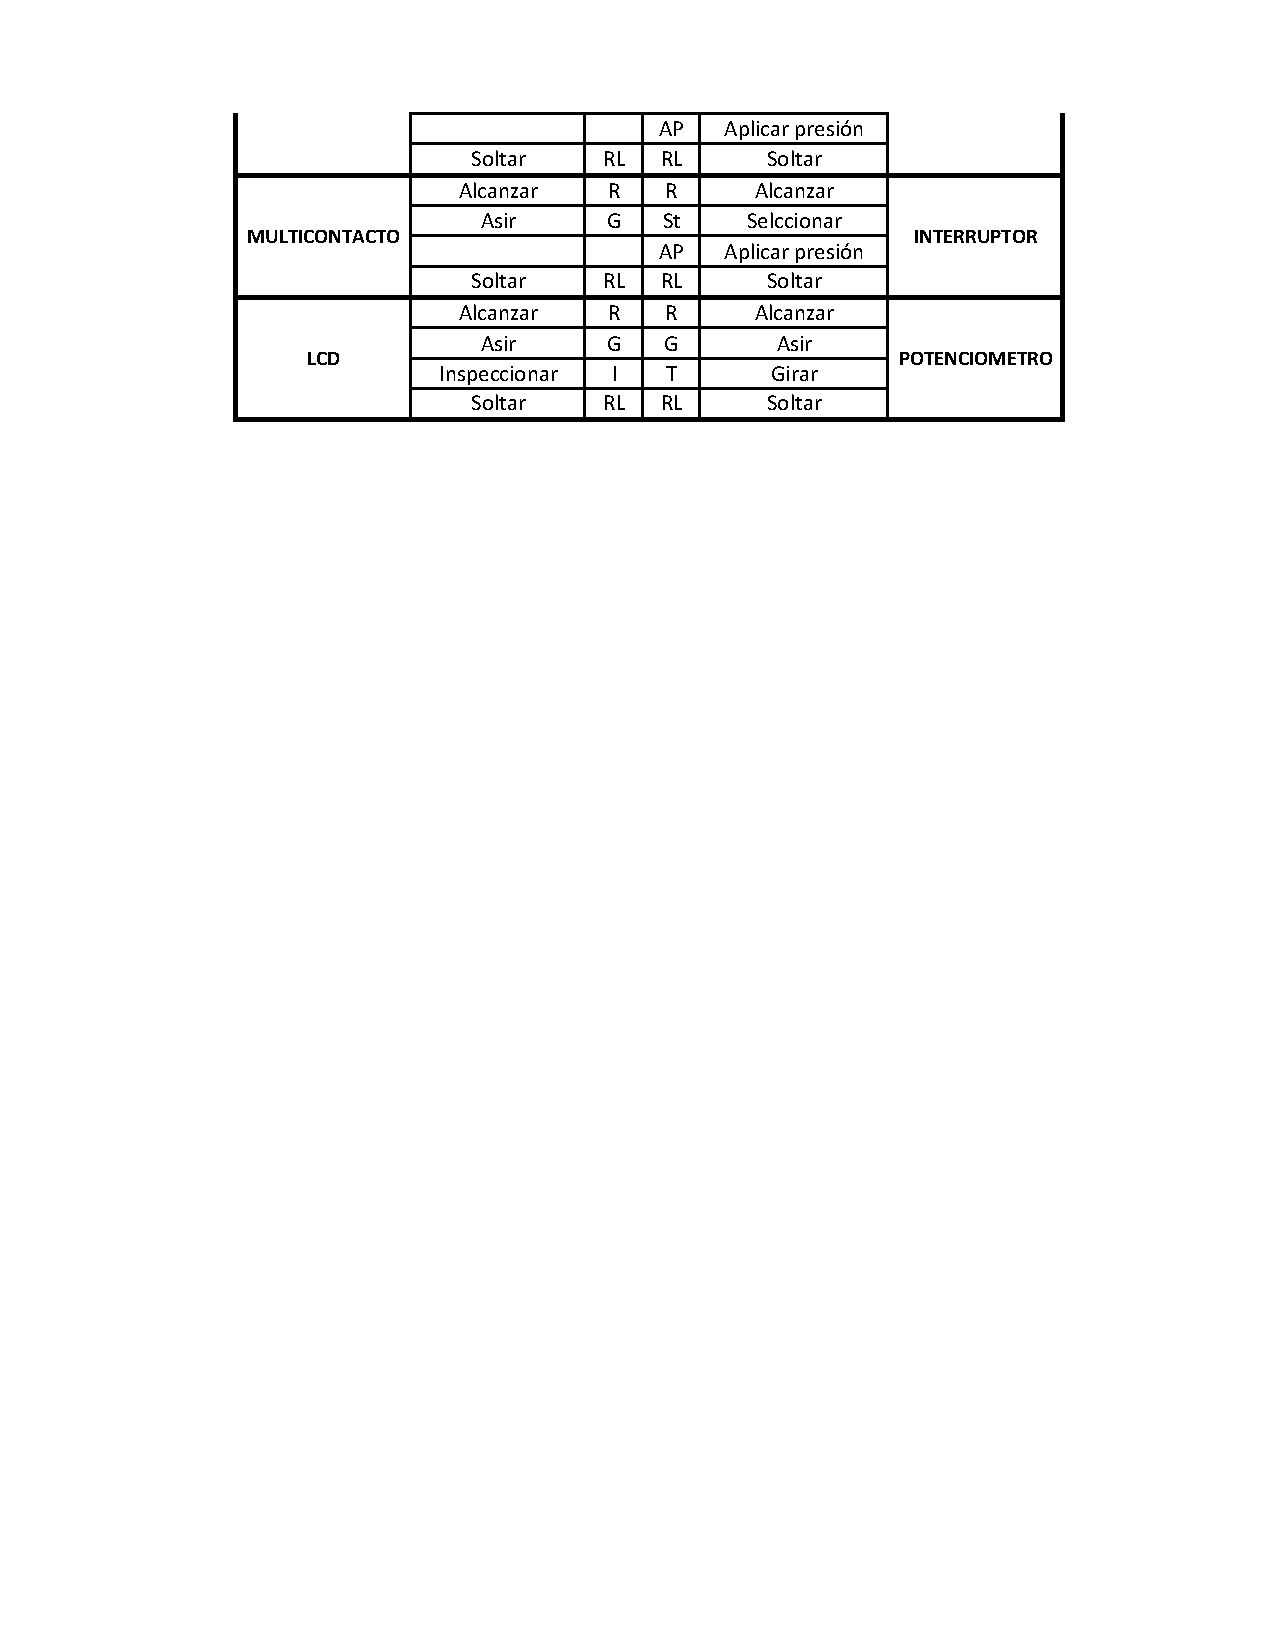
\includegraphics[trim = {5mm 15mm 5mm 10mm},clip,scale=0.3]{24/Img/diagramaBimanual3.pdf}
        \caption{}
        \label{fig:Diagrama Bimanual3}
    \end{figure}
    %
    \begin{figure}
        \centering
        \includegraphics[trim = {5mm 15mm 5mm 10mm},clip,scale=0.3]{24/Img/diagramaBimanual4.pdf}
        \caption{}
        \label{fig:Diagrama Bimanual4}
    \end{figure}
    %
    %
    \subsubsection{Verificación}
    
    
    Costos de no calidad.
    % 
    % 
    \subsubsection{Desarrollo del sistema de tiempos predeterminado}
    El desarrollo de un sistema de tiempos predeterminado consiste en la creación y aplicación de un conjunto de estándares de tiempo para realizar tareas específicas en un entorno de trabajo. Estos estándares se basan en estudios detallados de movimientos y tiempos necesarios para completar actividades laborales. El objetivo es establecer tiempos precisos y consistentes para mejorar la eficiencia, planificar la producción y establecer una base justa para la evaluación del desempeño y la determinación de salarios. Los sistemas de tiempos predeterminados ayudan a eliminar variaciones y asegurar que las tareas se realicen de manera eficiente y segura. En nuestro sistema de tiempos predeterminados obtuvimos con ayuda del TMU TOTAL, nuestro tiempo ciclo, el cual fue multiplicando 0.0006 que es lo equivalente a 1 TMU, por nuestro TMU TOTAL, para nuestro tiempo estándar multiplicamos el tiempo ciclo por uno mas el porcentaje de holgura el cual era de 0.14, así obteniendo los resultados mostrados en la tabla de análisis de MTM. (\ref{analisis1}, \ref{analisis2}, \ref{analisis3}, \ref{analisis4} ).
    %
    \begin{figure}
        \centering
    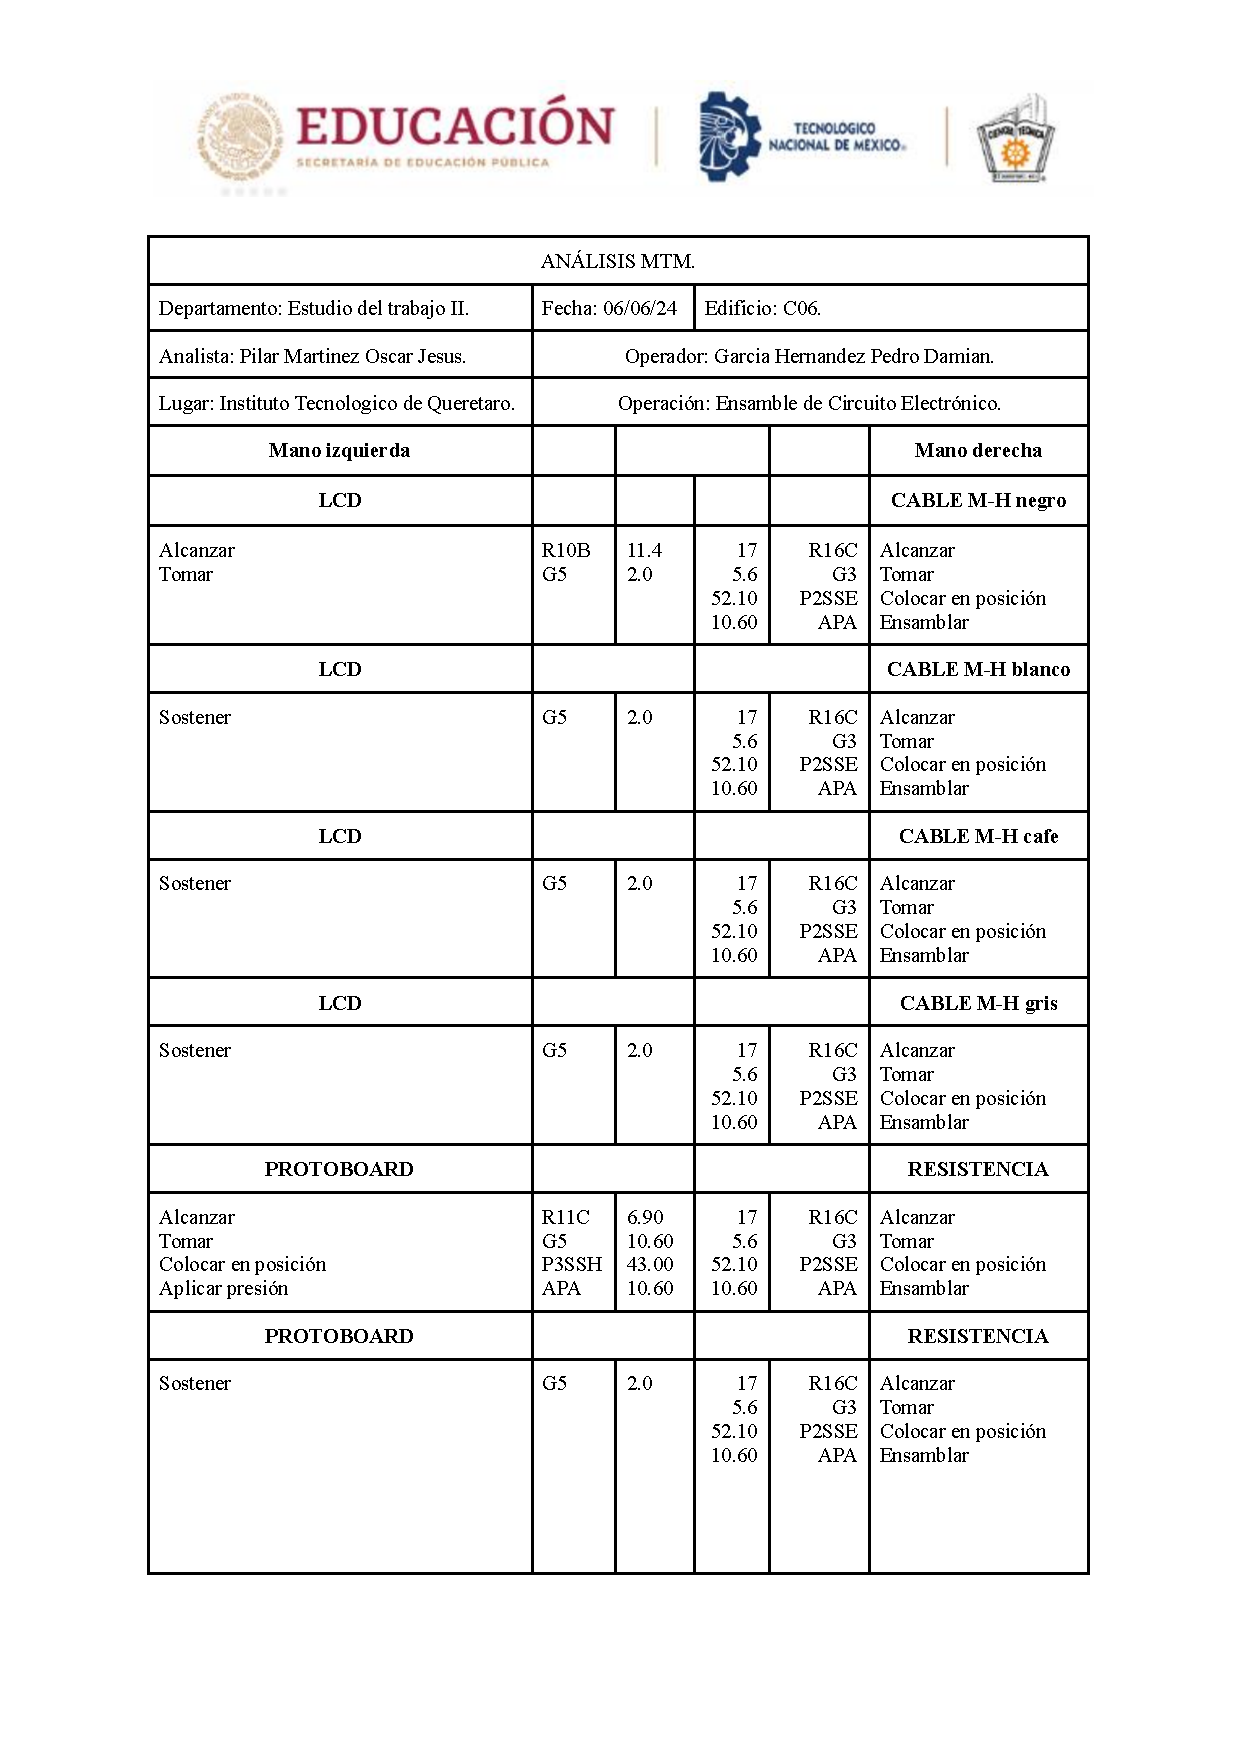
\includegraphics[trim = {0mm 0mm 0mm 0mm},clip,scale=0.3]{24/Img/analisisMTM1.pdf}
    \caption{ANÁLISIS DE MTM}
        \label{analisis1}
    \end{figure}
    %
    %
    \begin{figure}
        \centering
    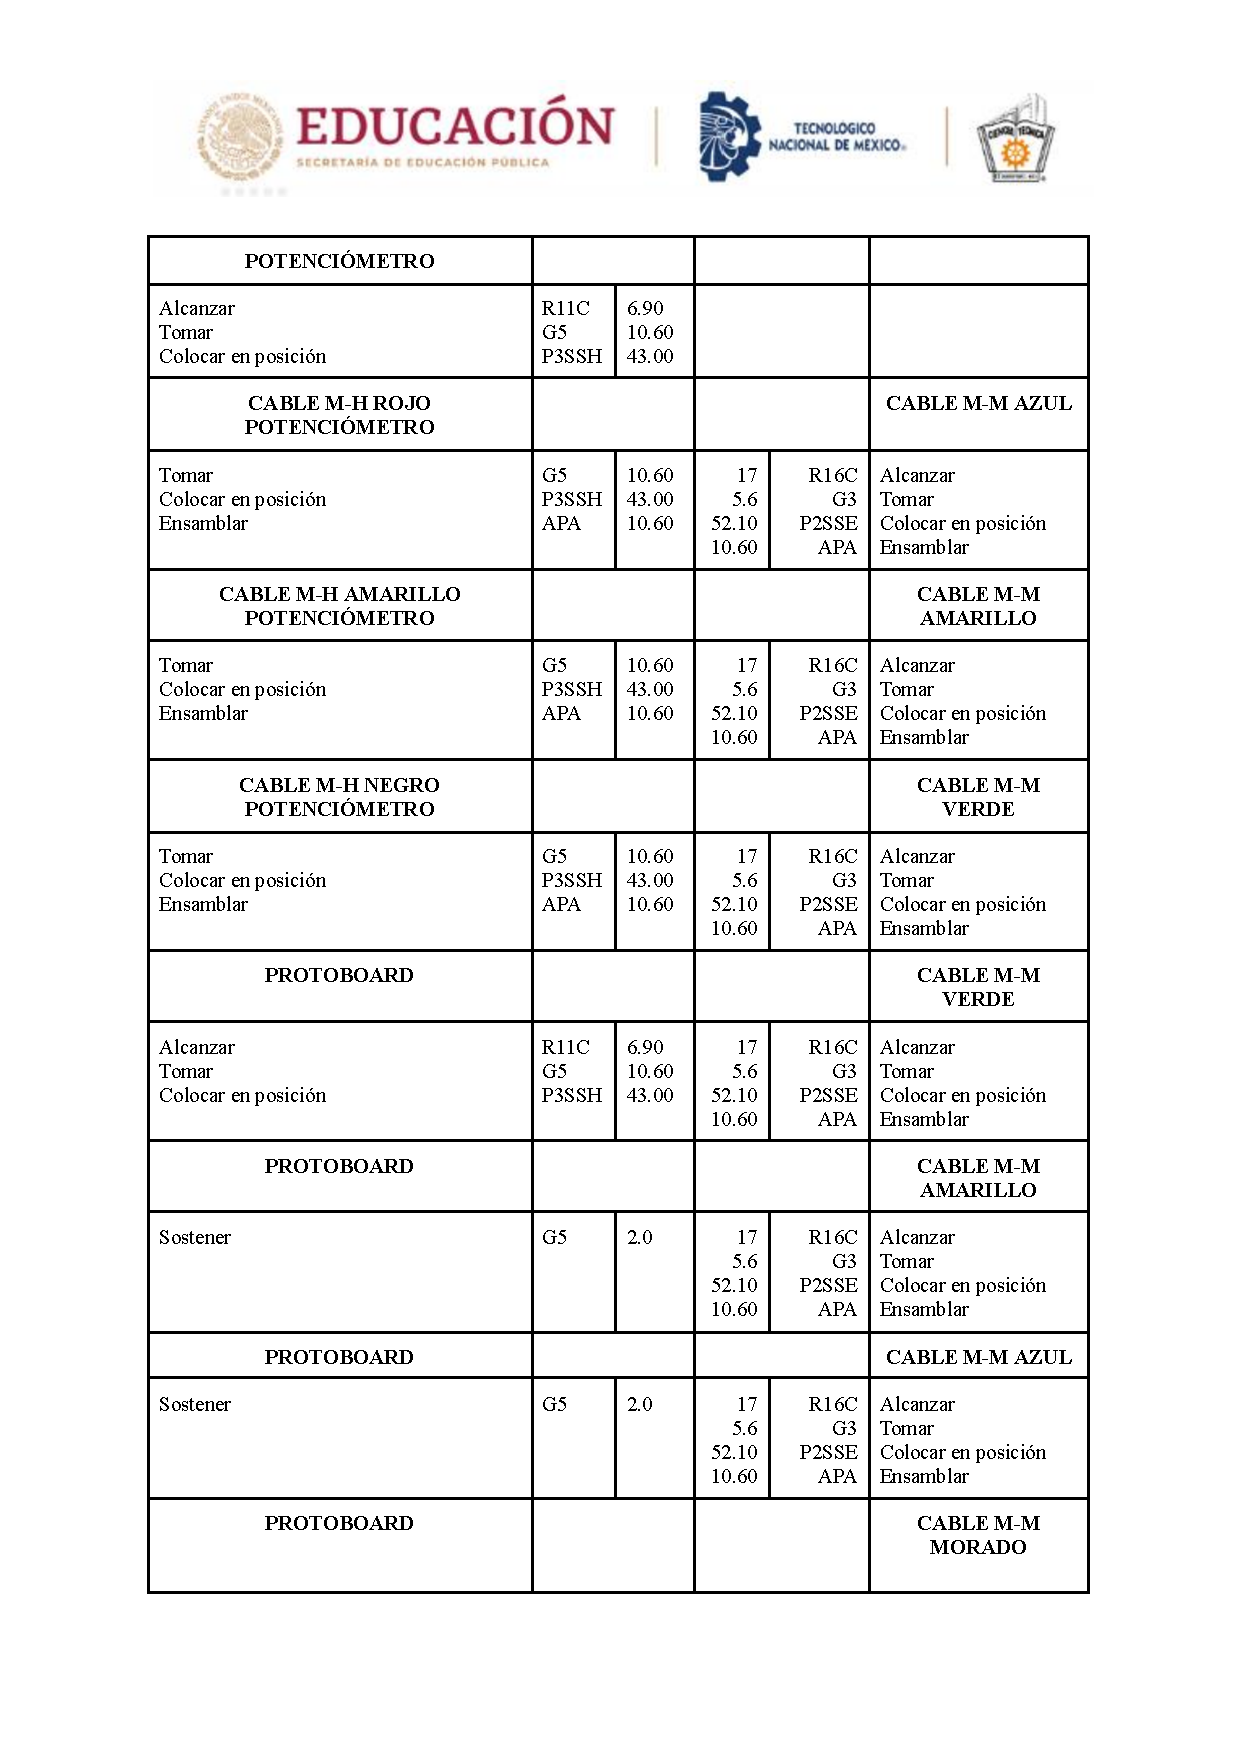
\includegraphics[trim = {0mm 0mm 0mm 0mm},clip,scale=0.3]{24/Img/analisisMTM2.pdf}
    \caption{ANÁLISIS DE MTM}
        \label{analisis2}
    \end{figure}
    %
    %
    \begin{figure}
        \centering
    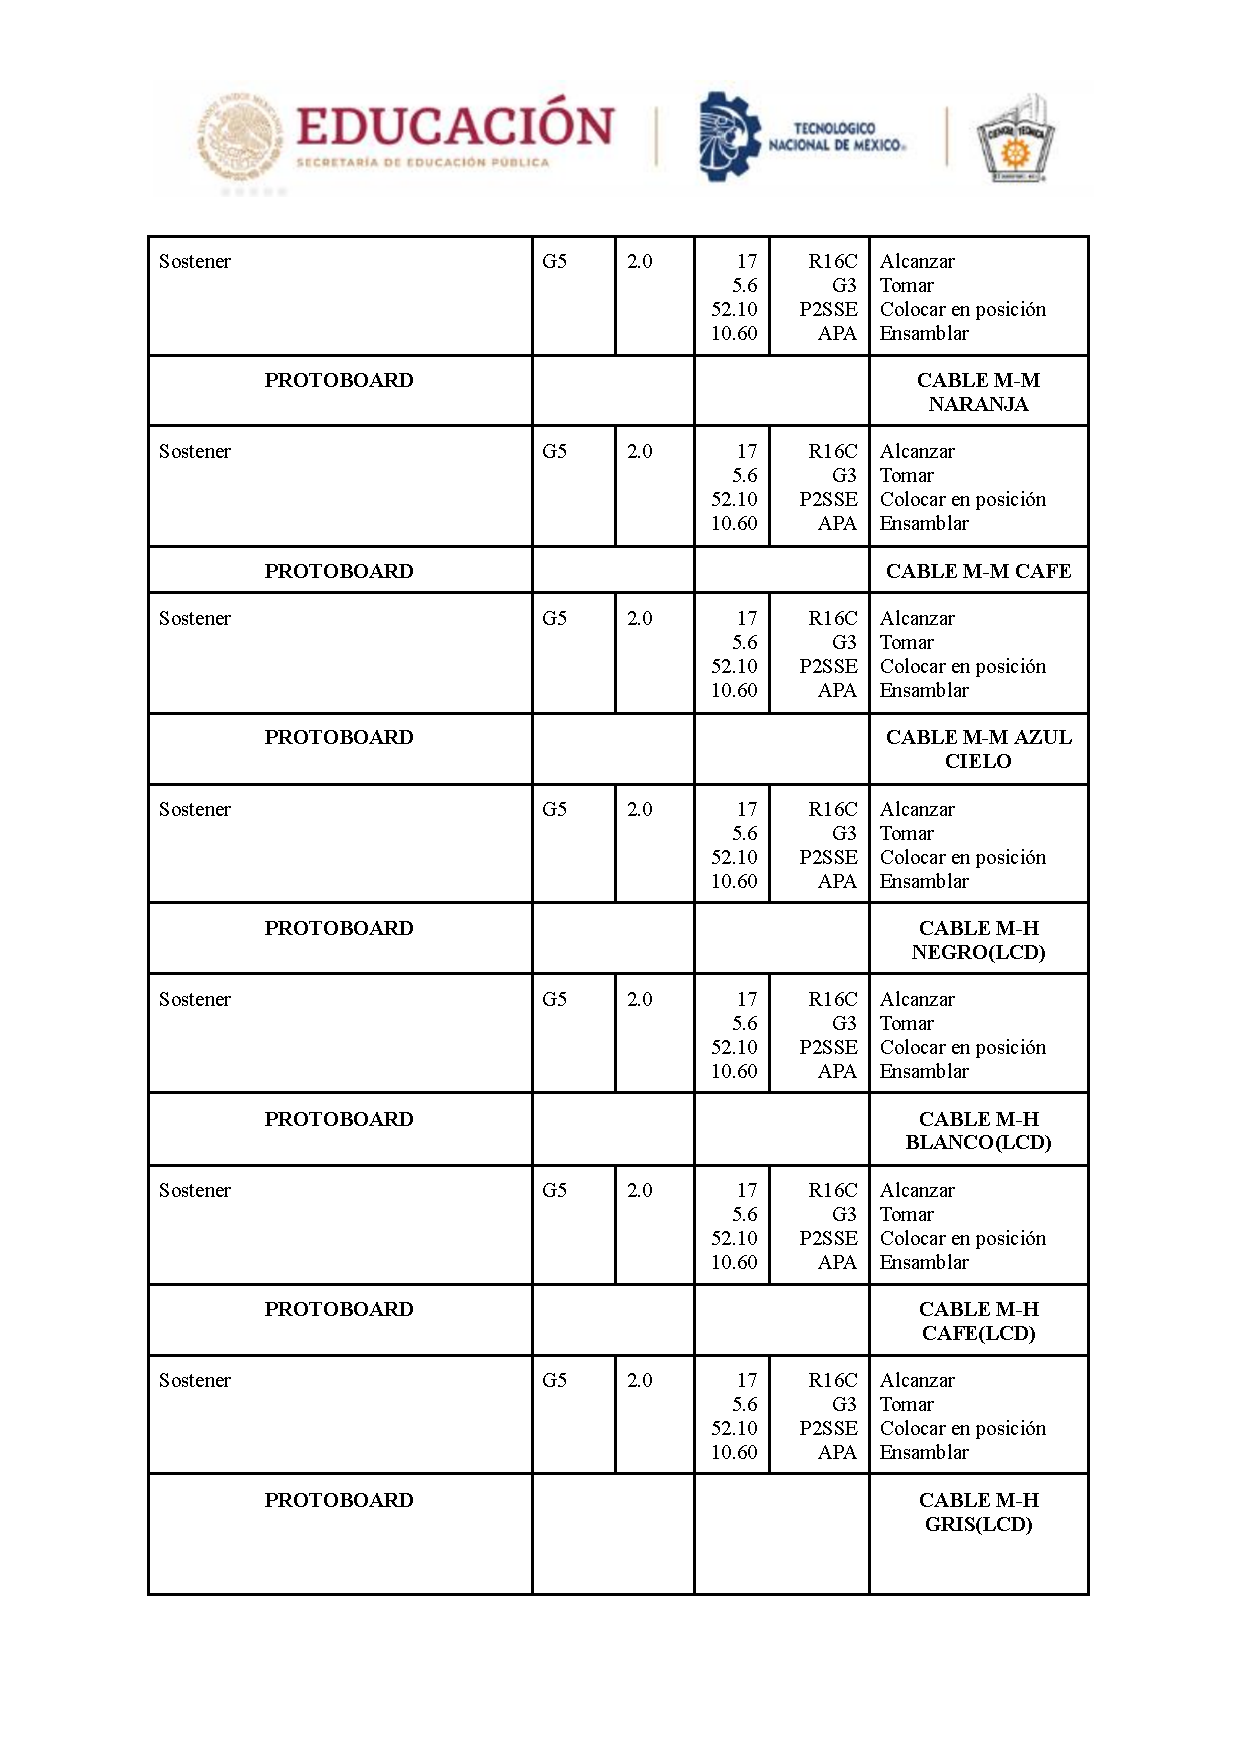
\includegraphics[trim = {0mm 0mm 0mm 0mm},clip,scale=0.3]{24/Img/analisisMTM3.pdf}
    \caption{ANÁLISIS DE MTM}
        \label{analisis3}
    \end{figure}
    %
    %
    \begin{figure}
        \centering
    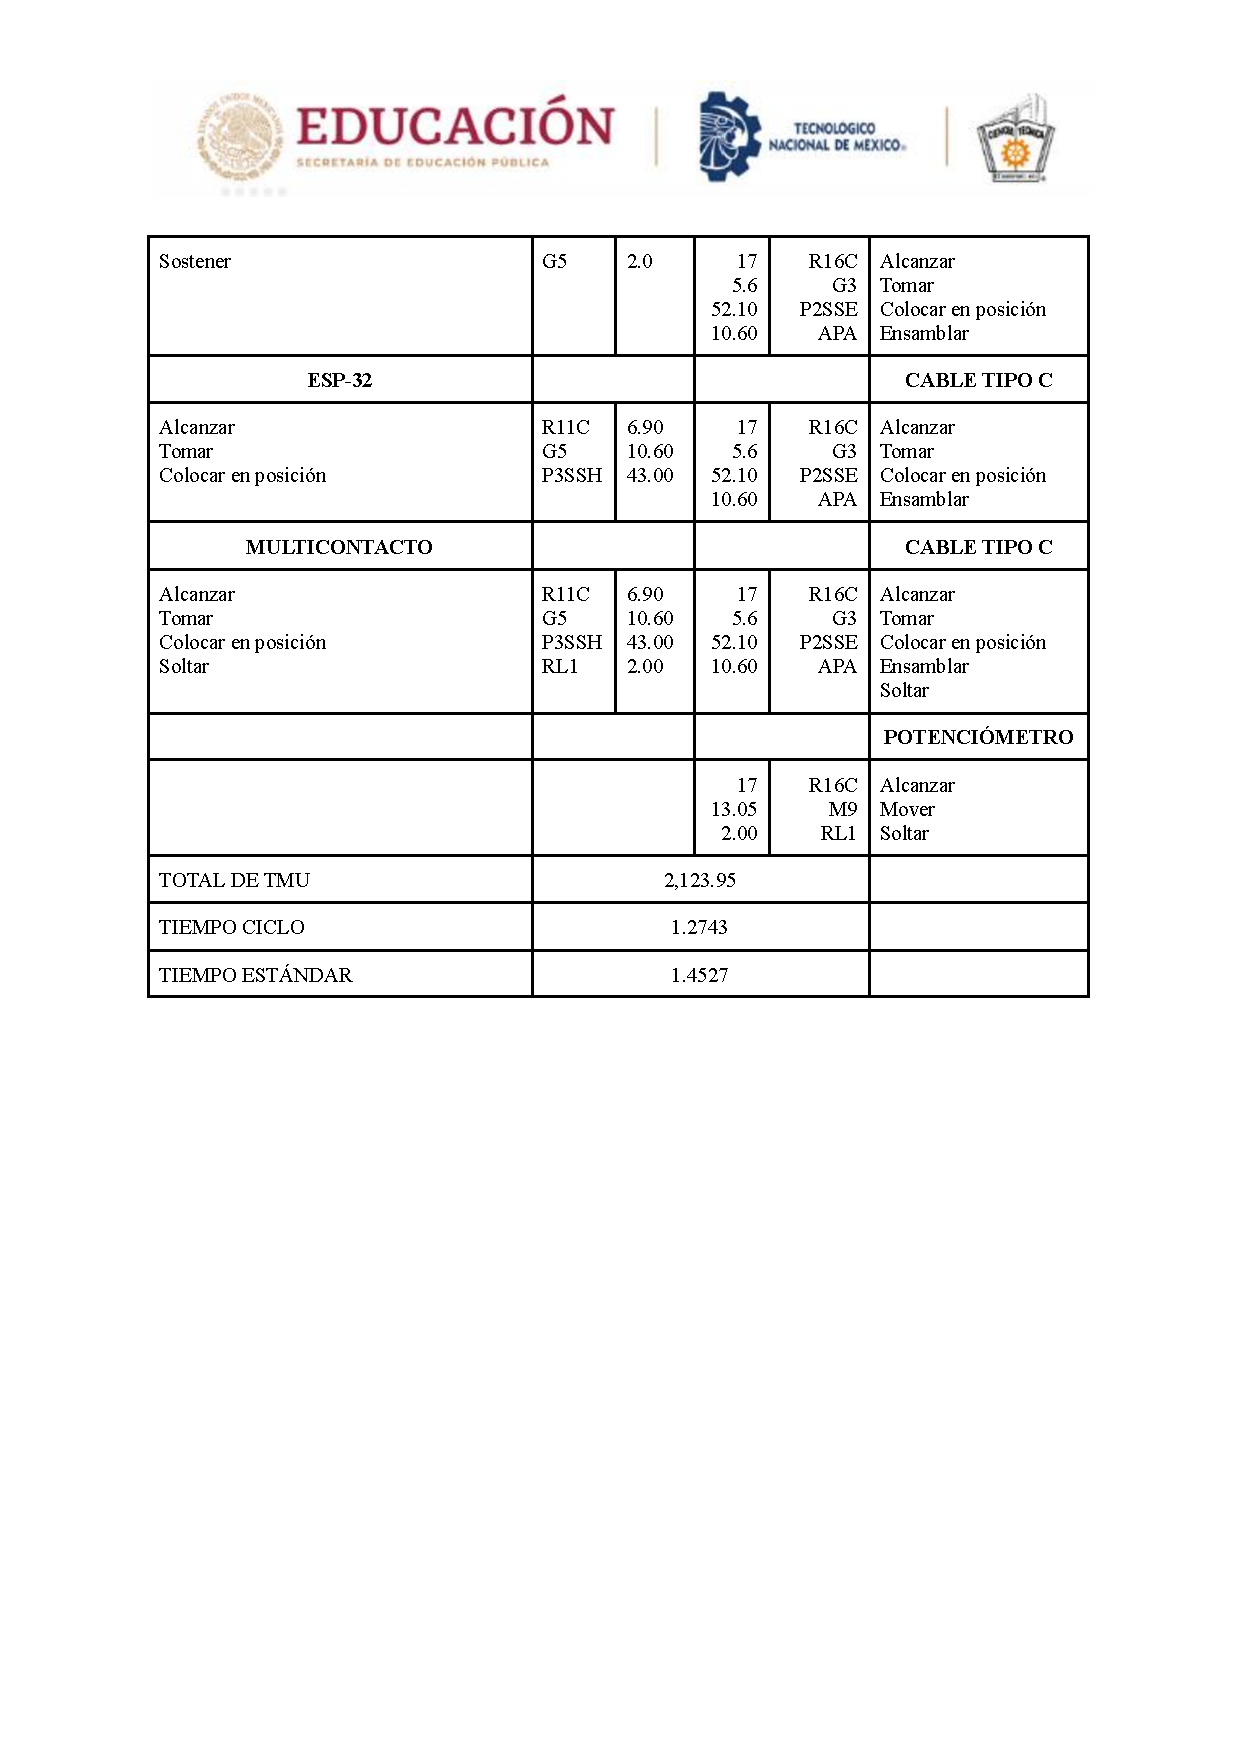
\includegraphics[trim = {0mm 100mm 0mm 0mm},clip,scale=0.3]{24/Img/analisisMTM4.pdf}
    \caption{ANÁLISIS DE MTM}
        \label{analisis4}
    \end{figure}
    %
    % 
    %
    \subsubsection{Desarrollo del muestreo del trabajo}
    El desarrollo del muestreo del trabajo implica la recopilación y análisis sistemático de datos sobre las actividades y tiempos de los trabajadores en un entorno de producción. Este proceso se lleva a cabo mediante la observación y registro de una muestra representativa de operaciones durante un período específico. El objetivo es identificar patrones, determinar tiempos estándar, y evaluar la eficiencia del trabajo. A través del muestreo del trabajo, se pueden identificar áreas de mejora, equilibrar cargas de trabajo, y optimizar procesos para reducir costos y aumentar la productividad.\ref{muestreo}
    %
    \begin{figure}
        \centering
    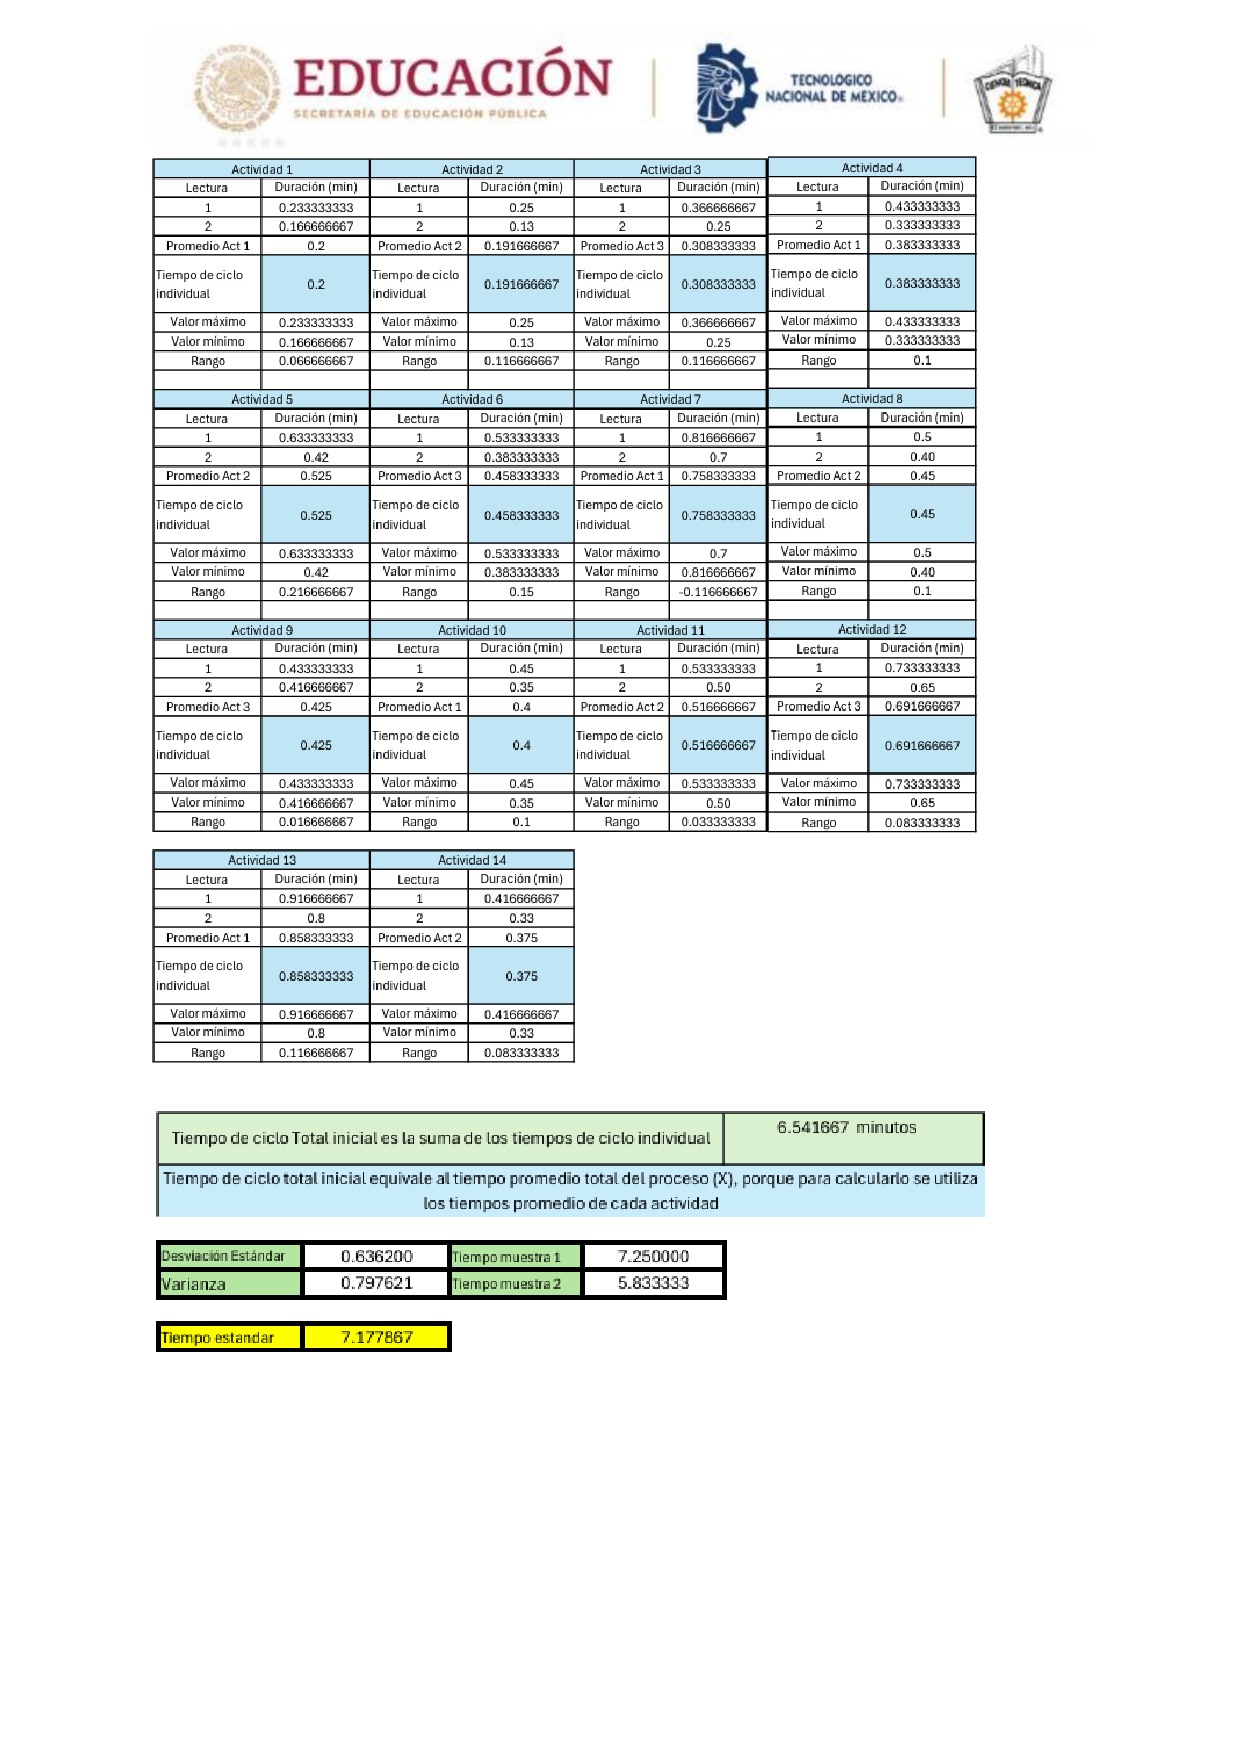
\includegraphics[trim = {0mm 0mm 0mm 0mm},clip,scale=0.3]{24/Img/muestreodeVideos2.pdf}
    \caption{DESARROLLO DEL MUESTREO}
        \label{muestreo}
    \end{figure}
    %
    % 
    % 
    \subsubsection{Corrección por balanceo de procesos}
    % 
    % 
    \subsubsection{Datos estándar continuos y discretos}
    % 
    % 
    \subsection{Diseño de la forma más económica de realizar el trabajo}
    
    % 
    % 
    \subsection{Normalización de los métodos, materiales, herramientas e instalaciones}
    
    % 
    % 
    \subsection{Determinación del tiempo estándar para que una persona competente realice el trabajo con marcha normal}
    
    
    % 
    % 
    \section{Conclusiones}
    A través del muestreo realizado, obtuvimos diversas muestras que fueron fundamentales para determinar nuestro tiempo estándar. Esto nos permitió identificar al operador promedio y al operador más lento. Posteriormente, pudimos realizar un balanceo de líneas, reduciendo así los tiempos de operación mediante el uso de therblings. Esto resultó en una disminución de nuestros costos operativos, logrando una producción balanceada y económica. Establecimos un tiempo estándar de 6 minutos para el ensamble aplicando sistemas de tiempos predeterminados (STP) y técnicas probabilísticas. Este enfoque nos permitió optimizar el estudio de movimientos y tiempos, identificando la manera más eficiente y económica de realizar el trabajo. 
    Con el desarrollo de este proyecto, alcanzamos los objetivos propuestos y adquirimos nuevas habilidades valiosas que se implementarán en futuros proyectos. En resumen, logramos mejorar la eficiencia y reducir costos, cumpliendo con las metas del estudio de movimientos y tiempos.
    
    
    %\section*{Referencias}
    %Para esta platilla, se solicita al autor enumerar las citas de manera consecutiva entre corchetes \cite{YLi2013}. 
    %La puntuación de la oración que sigues sería \cite{Mesaelides2011}. 
    %%Refiérase simplemente al número de referencia, como en \cite{Morales2012}, no utilice “Ref. [3]” o “referencia [3]” excepto al principio de una oración: “La referencia [3] fue la primera…”
    %Enumere las notas al pie por separado en superíndices. Coloque la nota de pie de en la parte inferior de la columna en la que se citó. No coloque notas al pie en la lista de referencias. Utilice letras para las notas al pie de la tabla.
    %A menos de que haya tres autores o más; no utilice “et al.”. Los trabajos que no hayan sido publicados, incluso si han sido presentados para su publicación, deben ser citados como “inéditos”. Los trabajos que han sido aceptados para su publicación deben de citarse como “en prensa”. Poner en mayúscula sólo la primera palabra de un título, excepto los nombres propios y los símbolos de elemento. 
    
    %Otros ejemplos \cite{LAAngeles2021}, \cite{LAAngelesConni}. 
    %
    % Ejemplo
    %  @Article{article,
    % 	author = "Author1 LastName1 and Author2 LastName2 and Author3 LastName3",
    % 	title = "Article Title",
    % 	volume = "30",
    % 	number = "30",
    % 	pages = "10127-10134",
    % 	year = "2013",
    % 	doi = "10.3389/fnins.2013.12345",
    % 	URL = "http://www.frontiersin.org/Journal/10.3389/fnins.2013.12345/abstract",
    % 	journal = "Frontiers in Neuroscience"
    % }
    
    % @book{book,
    %   author    = {Author Name}, 
    %   title     = {The title of the work},
    %   publisher = {The name of the publisher},
    %   address   = {The city},
    %   year      = 1993,
    % }
    
    % @incollection{chapter,
    %   author       = {Bauthor Surname}, 
    %   title        = {The title of the work},
    %   editor       = {Editor Name},
    %   booktitle    = {The title of the book},
    %   publisher    = {The name of the publisher},
    %   address      = {The city},
    %   year         = 2002,
    %   pages        = {201-213},
    % }
    
    % @InProceedings{conference,
    %   author = {Cauthor Name and Dauthor Surname and Fauthor LastName},
    %   title = {The title of the work},
    %   booktitle = {The title of the conference proceedings},
    %   year = 1996,
    %   publisher = {The name of the publisher},
    %   editor = {Editor Name1 and Editor Name2},
    %   pages = {41-50},
    % }
    
    % @book{cho,
    %   author       = {Gauthor Name1}, 
    %   title        = {The title of the work},
    %   publisher = {Country code and patent number},
    %   address      = {Patent Country},
    %   year = 2013
    % }
    
    % @book{patent,
    %   author    = {Hauthor Surname1}, 
    %   title     = {The title of the work},
    %   publisher = {Patent number},
    %   address   = {Patent country},
    %   year      = 2010,
    % }
    
    % % please use misc for datasets
    % @misc{dataset, 
    % 	author = "Author1 LastName1 and Author2 LastName2 and Author3 LastName3",
    % 	title = "Data Title",
    % 	year = "2011",
    % 	doi = "10.000/55555",
    % 	URL = "http://www.frontiersin.org/",
    % }
    
    \bibliographystyle{ieeetr}
    \bibliography{24/referencias}
    % 
    